\documentclass{article}

\title{
	Finding Optimal Diverse Feature Sets\\
	with Alternative Feature Selection
}
\author{
	Jakob Bach~\orcidlink{0000-0003-0301-2798}\\
	\small Karlsruhe Institute of Technology (KIT), Germany\\
	\small \href{mailto:jakob.bach@kit.edu}{jakob.bach@kit.edu}
}
\date{} % don't display a date

\usepackage[style=numeric, backend=bibtex]{biblatex}
\usepackage[ruled,linesnumbered,vlined]{algorithm2e} % pseudo-code
\usepackage{amsmath} % mathematical symbols
\usepackage{amssymb} % mathematical symbols
\usepackage{amsthm} % theorems, definitions etc.
\usepackage{booktabs} % nicely formatted tables (with top, mid, and bottom rule)
\usepackage{graphicx} % plots
\usepackage{orcidlink} % ORCID icon
\usepackage{subcaption} % figures with multiple sub-figures and sub-captions
\usepackage{hyperref} % links and URLs

\addbibresource{references.bib}

\newtheorem{corollary}{Corollary} % default theorem style ("plain")
\newtheorem{proposition}[corollary]{Proposition} % use joint numbering with corollaries
\theoremstyle{definition}
\newtheorem{definition}[corollary]{Definition}

\newcommand{\stirling}[2]{\genfrac\{\}{0pt}{}{#1}{#2}} % used for Stirling numbers of the second kind

\begin{document}

\maketitle

\begin{abstract}
Feature-selection methods are popular to obtain small, interpretable, yet highly accurate prediction models.
Existing feature-selection methods typically yield only one feature set, which might not be sufficient in some cases.
For example, users might be interested in finding different feature sets with similar prediction quality, offering alternative explanations of the data.
In this article, we introduce and formalize alternative feature selection as an optimization problem.
Next, we analyze the complexity of this optimization problem and show $\mathcal{NP}$-hardness.
Further, we discuss how to integrate various categories of existing feature-selection methods.
Finally, we evaluate alternative feature selection in a study with 30 classification datasets.
In our experiments, we observe that alternatives might indeed have similar prediction quality as the original feature sets, but several factors influence this outcome.
\end{abstract}
%
\textbf{Keywords:} feature selection, alternatives, constraints, mixed-integer programming, explainability, interpretability, XAI

\section{Introduction}
\label{sec:afs:introduction}

\paragraph{Motivation}

Feature-selection methods are ubiquitous for a variety of reasons.
By reducing dataset dimensionality, they lower the computational and memory requirements of prediction models.
Next, models might generalize better after removing irrelevant and spurious predictors.
Finally, prediction models might become simpler and more comprehensive~\cite{li2017feature}, improving interpretability.

Traditional feature-selection methods mostly return only one feature set~\cite{borboudakis2021extending}.
These methods optimize a criterion of feature-set quality, e.g., prediction performance.
However, besides the optimal feature set, there might be other, differently composed feature sets with similar quality.
For the user, such alternative feature sets might be interesting for multiple reasons.
First, some originally selected features might be costly to obtain, so the user would prefer cheaper alternatives.
Second, some originally selected features might contain sensitive information that should not be used in predictions.
Third, the user might be interested in explanations for the prediction, rather than just making good predictions.
In such a situation, knowing alternative feature sets allows the formulation of multiple, diverse explanations.
Such alternative explanations can broaden the user's understanding of the domain and help gain deeper insights.

\paragraph{Problem statement}

This article addresses the problem of alternative feature selection, which we informally define as follows:
%
\begin{definition}[Alternative feature selection (informal)]
	Given an original feature set, find a sufficiently different feature set that optimizes feature-set quality.
	\label{def:afs:alternative-feature-selection}
\end{definition}
%
We provide formal definitions in Section~\ref{sec:afs:approach:constraints}.
Ideally, the alternative feature set should have a similar quality as the original one.
However, depending on how different the alternative feature set should be, one might have to compromise on quality.
E.g., if there are only a few highly predictive features and most of them are part of the original feature set, the alternative feature set might have significantly lower prediction quality.
We analyze this effect in our article.
Also, we consider finding multiple alternatives rather than just one.

Two points are essential for alternative feature selection, which we both address in this article.
First, one needs to formalize and quantify what an alternative feature set is.
Second, one needs an approach to find alternative feature sets efficiently.
Ideally, the approach should be general, i.e., cover a broad range of existing feature-selection methods, given the variety of the latter~\cite{chandrashekar2014survey, li2017feature}.

\paragraph{Related work}

While finding alternative solutions has already been addressed extensively in the field of clustering~\cite{bailey2014alternative}, there is a lack of such approaches for feature selection.
Only few feature-selection methods target at obtaining multiple, diverse feature sets~\cite{borboudakis2021extending, siddiqi2020genetic}.
In particular, techniques for ensemble feature selection~\cite{saeys2008robust, seijo2017ensemble} and statistically equivalent feature subsets~\cite{lagani2017feature} produce multiple feature sets but not optimal alternatives.
In fields related to feature selection, the goal of obtaining multiple, diverse solutions has been studied as well, e.g., for subspace clustering~\cite{mueller2009relevant}, subspace search~\cite{trittenbach2019dimension}, or explainable-AI techniques~\cite{artelt2022even, kim2016examples, mothilal2020explaining, russell2019efficient} like counterfactuals.
However, these works address different problems than alternative feature selection, as we discuss in Section~\ref{sec:afs:related-work}.

\paragraph{Contributions}

Our contribution is fourfold.
First, we formalize alternative feature selection as an optimization problem.
In particular, we define alternatives via constraints on feature sets.
Also, we admit sequential as well as simultaneous search for multiple alternatives.
Second, we analyze the complexity of this optimization problem.
Third, we discuss approaches to solve the problem.
To that end, we describe how to integrate different categories of feature-selection methods in the objective function.
Fourth, we evaluate alternative feature selection with comprehensive experiments.
We use 30 classification dataset from the Penn Machine Learning Benchmarks (PMLB)~\cite{olson2017pmlb, romano2021pmlb} and five feature-selection methods.
We focus on the question if one can find alternative feature sets with similar feature-set quality as the original ones.

Our definition of alternatives is orthogonal to existing feature-selection methods, i.e., not tailored towards specific techniques.
Further, this formulation allows integrating other constraints on feature sets, e.g., based on domain knowledge~\cite{bach2022empirical, groves2015toward}.
Finally, we allow users to control the search for alternatives with two parameters, i.e., the number of alternatives and a dissimilarity threshold for feature sets being alternative.

\paragraph{Results}

From the theoretical perspective, we show that alternative feature selection is an $\mathcal{NP}$-hard optimization problem.
Experimentally, we could often find alternative feature sets with similar quality as the original ones.
Thereby, several factors influence the quality of alternatives, i.e., the dataset, feature-selection method, notion of feature-set quality, and the parameters for searching alternatives.
This outcome encourages using alternative feature sets as a tool for alternative explanations of predictions, though concrete statements on the quality of alternatives are up to the use case.
As expected, feature-set quality tends to decrease with the number of alternatives and dissimilarity threshold for being alternative.
Thus, these parameters allow the user to exercise use-case-specific control on the trade-off between feature sets being alternative and having high feature-set quality.
Also, depending on the number of features in the dataset, no valid alternatives might exist if the parameters values are too strict.
Computationally, a sequential search for alternatives was significantly faster than searching for multiple alternatives at once, while yielding a similar quality.
We publish our code\footnote{\url{https://github.com/Jakob-Bach/Alternative-Feature-Selection}} and our experimental data\footnote{\url{https://www.dropbox.com/sh/3bmeoihgozmvfg3/AAD9AcRddqRVlu7tps6FxIKIa?dl=0}} online. % TODO

\paragraph{Outline}

Section~\ref{sec:afs:fundamentals} explains fundamentals of feature selection.
Section~\ref{sec:afs:approach} defines the problem of alternative feature selection and discusses solution approaches.
Section~\ref{sec:afs:related-work} reviews related work.
Section~\ref{sec:afs:experimental-design} describes our experimental design and Section~\ref{sec:afs:evaluation} presents the experimental results.
Section~\ref{sec:afs:conclusion} concludes.
The appendix (cf.~Section~\ref{sec:afs:appendix}) contains complexity analyses, technical details, and approaches not used in our experiments.

\section{Fundamentals}
\label{sec:afs:fundamentals}

In this section, we introduce basic notation (cf.~Section~\ref{sec:afs:fundamentals:notation}) and review different methods to measure the quality of feature sets  (cf.~Section~\ref{sec:afs:fundamentals:quality}).

\subsection{Notation}
\label{sec:afs:fundamentals:notation}

Let $X \in \mathbb{R}^{m \times n}$ be a dataset represented as a matrix.
Each row is a data object, and each column is a feature.
Let $F = \{f_1, \dots, f_n\}$ denote the set of feature names.
We assume categorical features have already been made numeric, e.g., via one-hot encoding.
Let $X_{\cdot{}j} \in \mathbb{R}^m$ denote the vector representation of the $j$-th feature.
Further, let $y \in \mathbb{R}^m$ represent the prediction target.
The actual domain of the target might also be smaller, e.g., $\{0,1\}$ for binary classification.

With feature selection, one makes a binary decision $s_j \in \{0,1\}$ for each feature, i.e., either selects it or not.
The vector $s \in \{0,1\}^n$ combines all these selection decisions.
The selected feature set is $F_s = \{f_j \mid s_j=1\}$.
Let the function $Q(s,X,y)$ return the quality of such a feature set.
Without loss of generality, we assume this function should be maximized.

\subsection{Measuring Feature (Set) Quality}
\label{sec:afs:fundamentals:quality}

There are different ways to evaluate feature-set quality $Q(s,X,y)$.
Note that we only give a short overview here; see~\cite{chandrashekar2014survey,li2017feature} for comprehensive surveys of feature selection.
A traditional categorization of feature-selection methods distinguishes between filter, wrapper, and embedded methods~\cite{guyon2003introduction}.

\paragraph{Filter methods}

Filter methods evaluate feature sets without training a prediction model.
Univariate filters assess each feature independently, often assigning a score to each feature, while multivariate filters evaluate feature sets.
Examples for univariate filters are the absolute Pearson correlation or the mutual information between a feature and the prediction target.
Such methods ignore potential interaction between features, e.g., if they are redundant to each other.
In contrast, multivariate methods often combine a measure of feature relevance with a measure of feature redundancy.
Examples for such methods include CFS~\cite{hall1999correlation, hall2000correlation}, FCBF~\cite{yu2003feature}, and mRMR~\cite{peng2005feature}.
Another popular filter method is Relief~\cite{kira1992feature, robnik1997adaptation}, which assigns quality to individual features rather than feature sets but still uses other features indirectly in nearest-neighbor computations.

\paragraph{Wrapper methods}

Wrapper methods~\cite{kohavi1997wrappers} employ a generic search strategy over feature sets, e.g., genetic algorithms.
Feature-set quality is a black-box function:
Wrappers evaluate candidate feature sets from the search by training prediction models with them and measuring prediction quality.

\paragraph{Embedded methods}

Embedded methods train prediction models with built-in feature selection, e.g., decision trees~\cite{breiman1984classification} or random forests~\cite{breiman2001random}.
Thus, the criterion for feature-set quality is model-specific.
For example, tree-based models often use information gain or the Gini index to select features during training.

\paragraph{Post-hoc feature-importance methods}

Apart from traditional feature selection, there are various methods that assess feature importance after training a model.
These methods range range from local explanation methods like LIME~\cite{ribeiro2016should} or SHAP~\cite{lundberg2017unified} to global importance methods like permutation importance~\cite{breiman2001random} or SAGE~\cite{covert2020understanding}.
In particular, assessing feature importance plays a crucial role in the emerging field of ML interpretability~\cite{carvalho2019machine, molnar2020interpretable}.

\section{Alternative Feature Selection}
\label{sec:afs:approach}

In this section, we present the problem and approaches for alternative feature selection.
First, we define the structure of the optimization problem, i.e., objective and constraints (cf.~Section~\ref{sec:afs:approach:problem}).
Second, we formalize the notion of alternatives via constraints (cf.~Section~\ref{sec:afs:approach:constraints}).
Third, we discuss different objective functions, corresponding to different feature-set quality measures from Section~\ref{sec:afs:fundamentals:quality}.
In particular, we describe how to solve the resulting optimization problem (cf.~Section~\ref{sec:afs:approach:objectives}).
In addition, Appendix~\ref{sec:afs:appendix:complexity} analyzes the complexity of the optimization problem.

\subsection{Optimization Problem}
\label{sec:afs:approach:problem}

In alternative feature selection, there are two goals.
First, the quality of an alternative feature set should be high.
Second, an alternative feature set should differ from one or more existing feature set(s).
There are different ways to combine these two goals in an optimization problem:

First, one can consider both goals as objectives, obtaining an unconstrained multi-objective problem.
Second, one can treat feature-set quality as objective and enforce alternatives with constraints.
Third, one can consider being alternative as objective and constrain feature-set quality, e.g., with a lower bound.
Fourth, one can define constraints for both, feature-set quality and being alternative, searching for feasible solutions instead of optimizing.
Depending on the use case, any of these four formulations might be appropriate.

Following the informal Definition~\ref{def:afs:alternative-feature-selection} from the introduction, we stick to the second formulation, i.e., optimizing feature-set quality subject to being alternative.
This formulation has the advantage of keeping the original objective function of feature selection.
Consequently, one does not need to specify a range or a threshold on feature-set quality.
Instead, the user can control how alternative the new feature set should be.
This yields the following optimization problem:
%
\begin{equation}
	\begin{aligned}
		\max_s &\quad Q(s,X,y) \\
		\text{subject to:} &\quad F_s~\text{being alternative}
	\end{aligned}
	\label{eq:afs:afs-general}
\end{equation}
%
We discuss different constraints for \emph{being alternative} and different objective functions $Q(s,X,y)$ in the following.
Additionally, many feature-selection methods also limit the feature-set size $|F_s|$ to a user-defined value~$k \in \mathbb{N}$, as we do in our experiments as well.
Such a requirement on feature-set cardinality adds a further, simple constraint to the optimization problem.

\subsection{Constraints -- Defining Alternatives}
\label{sec:afs:approach:constraints}

In this section, we formalize alternative feature sets.
First, we discuss the base case where an individual feature set is an alternative to another one (cf.~Section~\ref{sec:afs:approach:constraints:single}).
Second, we extend this notion to multiple alternatives, considering sequential as well as simultaneous search procedures (cf.~Section~\ref{sec:afs:approach:constraints:multiple}).

Our notion of alternatives is independent of the feature-selection method.
We provide two parameters, i.e., a dissimilarity threshold~$\tau$ and the number of alternatives~$a$, which both allow users to control the search for alternatives.

\subsubsection{Single Alternative}
\label{sec:afs:approach:constraints:single}

We consider a feature set to be an alternative to another feature set if it differs sufficiently.
Mathematically, we express this with a set-dissimilarity measure~\cite{choi2010survey, egghe2009new}.
These measures typically assess how strongly two sets overlap and set this in relation to the size of the sets.
For example, a simple and well-known set-dissimilarity measure is the Jaccard distance.
Given two feature sets $F'$, $F''$, the Jaccard distance is defined as follows:
%
\begin{equation}
	d_{\text{Jacc}}(F',F'') = 1 - \frac{|F' \cap F''|}{|F' \cup F''|} = 1 - \frac{|F' \cap F''|}{|F'| + |F''| - |F' \cap F''|}
	\label{eq:afs:jaccard}
\end{equation}
%
Another possible dissimilarity measure follows from the Dice coefficient:
%
\begin{equation}
	d_{\text{Dice}}(F',F'') = 1 - \frac{2 \cdot |F' \cap F''|}{|F'| + |F''|}
	\label{eq:afs:dice}
\end{equation}
%
We do not have strong requirements on the set-dissimilarity measure~$d(\cdot)$.
Our definitions of alternatives only assume symmetry, i.e., $d(F',F'')=d(F'',F')$, and non-negativity, i.e., $d(F',F'') \geq 0$, though one could adapt them to other conditions as well.
In particular, the measure does not need to be a metric, but can also be a semi-metric~\cite{wilson1931semi} etc.

We leverage the set-dissimilarity measure for the following definition:
%
\begin{definition}[Single alternative]
	A feature set $F''$ is an alternative to a feature set $F'$ (and vice versa) for a dissimilarity threshold~$\tau \in \mathbb{R}_{\geq 0}$ if $d(F',F'') \geq \tau$.
	\label{def:afs:single-alternative}
\end{definition}
%
The threshold~$\tau$ controls how alternative the new feature set should be and depends on the dataset as well as the preferences of the user.
In particular, requiring the new feature set to differ strongly from the existing one might cause a significant drop in feature-set quality.
Some datasets might contain many features of similar utility, thereby enabling many alternatives of similar quality, while predictions on other datasets might depend on a few key features.
Only users can decide which drop in feature-set quality is acceptable for them as a trade-off for obtaining an alternative feature set.
Thus, we leave $\tau$ as a parameter.
In fact, it is the only parameter for our definition of single alternatives, unless one wants to vary the dissimilarity measure for feature sets as well.
In case the set-dissimilarity measure $d(\cdot)$ is normalized to $[0,1]$, like the Dice dissimilarity or Jaccard distance, the interpretation of $\tau$ is user-friendly:
Setting $\tau=0$ allows the alternative feature set to be identical to the original one, while $\tau=1$ requires the two feature sets to have no overlap.

If the choice of $\tau$ is unclear a priori, users can try out different values and compare results.
One potential approach is a binary search:
Start with the mid-range value of $\tau=0$, i.e., 0.5 for $\tau \in [0,1]$.
If the quality of the resulting alternative is too low, decrease $\tau$ to 0.25, i.e., allow more similarity.
If the quality of the resulting alternative is acceptably high, increase $\tau$ to 0.75, i.e., check a more dissimilar feature set.
Continue this procedure till an alternative with an acceptable quality-dissimilarity trade-off is found.

If the feature-set sizes $|F'|$ and $|F''|$ are known, a threshold~$\tau$ corresponds to a particular maximum number of overlapping features $|F' \cap F''|$.
This follows from re-arranging Equation~\ref{eq:afs:jaccard} and Equation~\ref{eq:afs:dice} in combination with Definition~\ref{def:afs:single-alternative}:
%
\begin{equation}
	\begin{aligned}
		d_{\text{Jacc}}(F',F'') = 1 - \frac{|F' \cap F''|}{|F'| + |F''| - |F' \cap F''|} &\geq \tau \\
		\Leftrightarrow |F' \cap F''| &\leq \frac{1 - \tau}{2 - \tau} \cdot (|F'| + |F''|)
		\end{aligned}
	\label{eq:afs:jaccard-rearranged}
\end{equation}
%
The latter formulation also avoids having the feature-set sizes, and thereby the decision variables for feature selection, in a quotient.
However, the effect of $\tau$ on the maximum overlap size $|F' \cap F''|$ is non-linear for the Jaccard distance in Equation~\ref{eq:afs:jaccard-rearranged}.
Thus, we use the Dice dissimilarity in this article, where the effect of $\tau$ on the maximum overlap size $|F' \cap F''|$ is linear:
%
\begin{equation}
	\begin{aligned}
		d_{\text{Dice}}(F',F'') = 1 - \frac{2 \cdot |F' \cap F''|}{|F'| + |F''|} &\geq \tau \\
		\Leftrightarrow |F' \cap F''| &\leq \frac{1 - \tau}{2} \cdot (|F'| + |F''|)
	\end{aligned}
	\label{eq:afs:dice-rearranged}
\end{equation}
%
If $|F'| = |F''|$, as in our experiments, the measure becomes identical to several other dissimilarity measures~\cite{egghe2009new}.
Further, $\tau$ then directly controls which fraction of features in one set needs to differ from the other set, and vice versa:
%
\begin{equation}
	\begin{aligned}
		\text{If}~|F'| = |F''|: \quad d_{\text{Dice}}(F',F'') &\geq \tau \\
		\Leftrightarrow |F' \cap F''| &\leq (1 - \tau) \cdot |F'| = (1 - \tau) \cdot |F''|
	\end{aligned}
	\label{eq:afs:dice-rearranged-equal-size}
\end{equation}
%
Thus, if users are uncertain how to choose $\tau$ and $|F''|$ is reasonably small, they can try out all values of $\tau \in \{i / |F''|\}$ with $i \in \{0, 1, \dots, |F''|\}$.
Put differently, $|F''| + 1$ values of $\tau$ cover all potential overlap sizes of the two feature sets.

Up to now, we have used feature sets instead of the binary feature-selection vector $s$.
However, expressing the feature-set sizes in terms of $s$ is straightforward:
%
\begin{equation}
	\begin{aligned}
		|F_s| =& \sum_{j=1}^n s_j \\
		|F_{s'} \cap F_{s''}| =& \sum_{j=1}^n s'_j \cdot s''_j
	\end{aligned}
	\label{eq:afs:feature-set-size}
\end{equation}
%
The expression from Equation~\ref{eq:afs:feature-set-size} also helps to formulate a constraint for limiting the new feature set's size to a user-defined value~$k \in \mathbb{N}$.
Further, combining Equation~\ref{eq:afs:jaccard-rearranged},~\ref{eq:afs:dice-rearranged},~or~\ref{eq:afs:dice-rearranged-equal-size} with Equation~\ref{eq:afs:feature-set-size} yields an inequality only involving sums and products of the binary decision variables and constant values.
In fact, one can replace the product $s'_j \cdot s''_j$, which is non-linear, with linear constraints by introducing an auxiliary variable $t_j$~\cite{mosek2022modeling} as follows:
%
\begin{equation}
	\begin{aligned}
		t_j \leq& s'_j \\
		t_j \leq& s''_j \\
		1 + t_j \geq& s'_j + s''_j \\
		t_j \in& \{0,1\}
	\end{aligned}
	\label{eq:afs:product-linear}
\end{equation}
%
If there is an existing feature set, i.e., either $s'$ or $s''$ is fixed to particular values, Equation~\ref{eq:afs:feature-set-size} already is linear without Equation~\ref{eq:afs:product-linear} since it only multiplies variables with constants in that case.

Overall, one can express alternative feature sets following Definition~\ref{def:afs:single-alternative} with 0-1 integer linear constraints.
This simple constraint type allows using a broad range of solvers, given a suitable objective function, which we discuss later.
One can also encode such constraints into propositional logic (\textsc{SAT})~\cite{ulrich2022selecting}.

\subsubsection{Multiple Alternatives}
\label{sec:afs:approach:constraints:multiple}

If the user desires multiple alternative feature sets rather than only one, we can compute these alternatives either sequentially or simultaneously.
The number of alternatives~$a$ is a parameter to be set by the user.
Table~\ref{tab:afs:seq-sim-comparison} compares the sizes of the optimization problems for these two search procedures.
Appendix~\ref{sec:afs:appendix:complexity} analyzes the computational complexity of the optimization problems in detail.
In particular, we show $\mathcal{NP}$-hardness for simultaneous search (cf.~Corollary~\ref{corr:afs:complexity-sim}).
%
\begin{table}[htb]
	\centering
	\renewcommand*{\arraystretch}{1.3}
	\begin{tabular}{lccc}
		\toprule
		& \multicolumn{2}{c}{Sequential search} & Simultaneous search \\
		\cmidrule(r){2-3}
		& Alternative $i$ & Summed & \\
		\midrule
		Decision variables~$s$ & $n$ & $ (a+1) \cdot n$ & $(a+1) \cdot n$ \\
		Linearization variables~$t$ & $0$ & $0$ & $\frac{a \cdot (a+1) \cdot n}{2}$ \\
		Alternative constraints & $i$ & $\frac{a \cdot (a+1)}{2}$ & $\frac{a \cdot (a+1)}{2}$ \\
		Linearization constraints & $0$ & $0$ & $\frac{3 \cdot a \cdot (a+1) \cdot n}{2}$ \\
		\bottomrule
	\end{tabular}
	\caption{Size of the optimization problems for $a$ alternatives ($a + 1$~feature sets overall, including the original one) and $n$ features.}
	\label{tab:afs:seq-sim-comparison}
\end{table}
%
\paragraph{Sequential alternatives}

In the sequential case, the user gets several alternatives iteratively, with one alternative feature set per iteration.
We constrain this new feature set to be an alternative to all previously found feature sets:
%
\begin{definition}[Sequential alternative]
	A feature set $F''$ is an alternative to a set of feature sets $\mathbb{F}$ (and vice versa) for a dissimilarity threshold~$\tau \in \mathbb{R}_{\geq 0}$ if $\forall F' \in \mathbb{F}: d(F',F'') \geq \tau$.
	\label{def:afs:sequential-alternative}
\end{definition}
%
This definition duplicates the constraint for a single alternative (cf.~Definition~\ref{def:afs:single-alternative}) and instantiates it for multiple existing feature sets.
One could also use a less strict constraint, e.g., based on aggregated dissimilarity, like requiring only the average dissimilarity to all existing feature sets to pass the threshold.
However, definitions like the latter might allow some feature sets to heavily overlap or even be identical if other feature sets are very dissimilar.
Thus, we require pairwise dissimilarity in Definition~\ref{def:afs:sequential-alternative}.
We obtain the following optimization problem, letting $\mathbb{F}$ denote the set of existing feature sets:
%
\begin{equation}
	\begin{aligned}
		\max_s &\quad Q(s,X,y) \\
		\text{subject to:} &\quad \forall F' \in \mathbb{F}: d(F_s,F') \geq \tau
	\end{aligned}
	\label{eq:afs:afs-sequential}
\end{equation}
%
The objective function remains the same as for a single alternative ($|\mathbb{F}| = 1$), i.e., we only optimize the quality of the new feature set~$F_s$.
Thus, the number of variables in the optimization problem is independent of the number of alternatives~$a$.
Instead, we solve the optimization problem repeatedly; each alternative only adds one new constraint to the problem.
As we always compare the new, variable feature set to existing, constant feature sets, we also do not need to introduce interaction variables as in Equation~\ref{eq:afs:product-linear}.
Overall, we expect the runtime of sequential search to scale well with the number of alternatives.
Further runtime gains might be possible if the solver keeps a state between iterations and can warm-start.

However, as the solution space becomes narrower over iterations, feature-set quality can deteriorate with each further alternative.
In particular, multiple alternatives from the same sequential search might differ significantly in their quality.
As a remedy, the user can decide after each iteration if the feature-set quality already is unacceptably low or if another alternative should be found.
In particular, the user does not need to define the number of alternatives~$a$ a priori.

\paragraph{Simultaneous alternatives}

In the simultaneous case, we directly obtain multiple alternatives.
Thus, the user needs to decide on the number of alternatives beforehand.
We formulate pairwise dissimilarity constraints:
%
\begin{definition}[Simultaneous alternatives]
	A set of feature sets $\mathbb{F}$ contains simultaneous alternatives for a dissimilarity threshold~$\tau \in \mathbb{R}_{\geq 0}$ if $\forall F' \in \mathbb{F}, F'' \in \mathbb{F}, F' \neq F'': d(F',F'') \geq \tau$.
	\label{def:afs:simultaneous-alternative}
\end{definition}
%
This definition leads to the following optimization problem, assuming we want to obtain $a$ alternative feature sets besides an `original' feature set.
Since there is no order of feature sets here, opposed to sequential search, the original feature set is no dedicated feature set but can be any of the solutions.
%
\begin{equation}
	\begin{aligned}
		\max_{s^{(0)}, \dots, s^{(a)}} &\quad \operatorname*{agg}_{i \in \{0, \dots, a\}} Q(s^{(i)},X,y) \\
		\text{subject to:} &\quad \forall i_1 \in \{1, \dots, a\}~\forall i_2 \in \{0, \dots, i_1-1\}: d(F_{s^{(i_1)}},F_{s^{(i_2)}}) \geq \tau
	\end{aligned}
	\label{eq:afs:afs-simultaneous}
\end{equation}
%
In contrast to the sequential case, we need to introduce further decision variables and modify the objective function here, as we optimize multiple feature sets at once.
The operator~$\text{agg}(\cdot)$ defines how to aggregate the qualities of these feature sets in the objective.
In our experiments, we consider the sum as well as the minimum for aggregation.
Appendix~\ref{sec:afs:appendix:simultaneous-objective-aggregation} discusses these two aggregation functions and ideas for further formulations in detail.

Runtime-wise, we expect simultaneous search to scale worse with the number of alternatives than sequential search, as we need to tackle one large optimization problem instead of multiple smaller ones.
In particular, the number of decision variables increases linearly with the number of alternatives~$a$ and the number of constraints even grows quadratically.
Also, for each feature and each pair of alternatives, we need to introduce an interaction variable as in Equation~\ref{eq:afs:product-linear} if we want to obtain a linear problem.

In contrast to the greedy procedure of sequential search, simultaneous search optimizes alternatives globally.
Thus, the simultaneous procedure should yield same or higher average feature-set quality for the same number of alternatives.
Also, the quality can be more evenly distributed over the alternatives, as opposed to the dropping quality over the course of the sequential procedure.
However, increasing the number of alternatives still has a negative effect on the average feature-set quality.
Further, opposed to the sequential procedure, there are no intermediate steps where the user could interrupt the search.

\subsection{Objective Functions -- Finding Alternatives}
\label{sec:afs:approach:objectives}

In this section, we present approaches for finding alternative feature sets.
We discuss how to solve the optimization problem from Section~\ref{sec:afs:approach:problem} for the different categories of feature-set quality measures from Section~\ref{sec:afs:fundamentals:quality}.
In particular, we categorize solution approaches as white-box optimization (cf.~Section~\ref{sec:afs:approach:objectives:white-box}), black-box optimization (cf.~Section~\ref{sec:afs:approach:objectives:black-box}), and embedding alternatives (cf.~Section~\ref{sec:afs:approach:objectives:embedding}).

\subsubsection{White-Box Optimization}
\label{sec:afs:approach:objectives:white-box}

If the feature-set quality function~$Q(s,X,y)$ is sufficiently simple, one can tackle alternative feature selection with a suitable white-box solver.
In Section~\ref{sec:afs:approach:constraints}, we already showed that our notion of alternative feature sets results in 0-1 integer linear constraints.
In this section, we present white-box optimization objectives for different feature-selection methods.

\paragraph{Univariate filter feature selection}

For univariate filter feature selection, the objective function is linear.
Thus, the optimization problem of alternative feature selection becomes a 0-1 integer linear problem.

In particular, univariate filter methods decompose the quality of a feature set into the quality of the individual features:
%
\begin{equation}
	Q_{\text{uni}}(s,X,y) = \sum_{j=1}^{n} q(X_{\cdot{}j},y) \cdot s_j
	\label{eq:afs:univariate-filter}
\end{equation}
%
Here, $q(\cdot)$ typically is a bivariate dependency measure, e.g., mutual information~\cite{kraskov2004estimating} or absolute value of Pearson correlation, to quantify the relationship between one feature and the prediction target.
Thus, the values of~$q(\cdot)$ for different features are independent from each other.
Appendix~\ref{sec:afs:appendix:complete-optimization-problem} specifies the complete optimization problem including the constraints for alternatives.
Appendix~\ref{sec:afs:appendix:univariate-search-algorithm} presents a procedure to tackle the problem without a solver.

Alternatively, one could formulate a weighted partial maximum satisfiability (\textsc{MaxSAT}) problem~\cite{bacchus2021maximum, li2021maxsat}, in particular, a weighted \textsc{Max One} problem~\cite{khanna1997complete}, since the univariate objective only is a sum of weighted binary variables.
One would need to apply a cardinality encoding~\cite{sinz2005towards} for the constraints involving~$k$.

\paragraph{Post-hoc feature importance}

From the technical perspective, one can also insert values of post-hoc feature-importance scores into Equation~\ref{eq:afs:univariate-filter}.
For example, one can pre-compute permutation importance~\cite{breiman2001random} or SAGE scores~\cite{covert2020understanding} for each feature and use them instead of the bivariate dependency values~$q(X_{\cdot{}j},y)$.
However, such post-hoc importance scores often evaluate the usefulness of each feature in the presence of other features.
Thus, importance scores of different features are not independent from each other, violating the assumption behind Equation~\ref{eq:afs:univariate-filter}.
For example, a feature might show high post-hoc importance if another feature is present, due to feature interaction, but low importance else.
Equation~\ref{eq:afs:univariate-filter} cannot express such conditional importance but requires one overall quality value for each feature.

In theory, one would have to re-calculate feature importance for each possible set of selected features to capture all possible feature interactions.
However, such a procedure demands extensive runtime, scales exponentially with the number of features, and makes white-box optimization infeasible.
In practice, one can use Equation~\ref{eq:afs:univariate-filter} with importance scores only computed on the full dataset, i.e., with all feature being present.
One only needs to be aware that such an approach might not represent importances in feature subsets faithfully.

\paragraph{Multivariate filter feature selection}

Several multivariate filter methods allow for a simple white-box formulation as well, though not necessarily a linear one.
In the following, we describe FCBF~\cite{yu2003feature} and mRMR~\cite{peng2005feature}, which we use in our experiments.
Appendix~\ref{sec:afs:appendix:multivariate-filter-objectives}~discusses CFS~\cite{hall1999correlation, hall2000correlation} and and Relief~\cite{kira1992feature, robnik1997adaptation}.

\paragraph{FCBF}

The Fast Correlation-Based Filter (FCBF)~\cite{yu2003feature} bases on the notion of predominance, expressed by two conditions on selected features:
First, a selected feature's correlation to the prediction target needs to pass a pre-defined threshold.
Second, a selected feature's correlation to the target needs to be higher than each other selected feature's correlation to the given feature.
While the original FCBF algorithm uses a heuristic search to find predominant features, we propose a formulation as a constrained optimization problem:
%
\begin{equation}
	\begin{aligned}
		\max_s &\quad & Q_{\text{FCBF}}(s,X,y) &= \sum_{j=1}^{n} q(X_{\cdot{}j},y) \cdot s_j \\
		\text{subject to:} &\quad \forall j_1 \forall j_2 & \text{with } q(X_{\cdot{}j_1},y) &\leq q(X_{\cdot{}j_2}, X_{\cdot{}j_1}): \\
		&\quad & s_{j_1} + s_{j_2} &\leq 1 \\
		\text{with indices:} &\quad & j_1 &\in \{2, \dots, n\} \\
		&\quad & j_2 &\in \{1, \dots, j_1 - 1\}
	\end{aligned}
	\label{eq:afs:fcbf}
\end{equation}
%
Our formulation still addresses the two aspects of predominance.
First, we drop the original FCBF's threshold parameter on feature-target correlation and maximize the latter instead, as in the univariate-filter case.
This change can lead to large feature sets, which might containing many low-quality features.
As a countermeasure, one can add a constraint on the feature-set size, as we do in our experiments.
If one still wants to prevent the selection of features with low correlation to the prediction target, one can also filter out these features before optimization.
Second, we keep FCBF's constraints on feature-feature correlation.
In particular, we prevent the simultaneous selection of two features if the correlation between them is at least as high as one of the features' correlation to the target.
As the if-condition in Equation~\ref{eq:afs:fcbf} does not depend on the decision variables~$s$, one can pre-compute whether it holds and add the related linear constraint on~$s$ only if needed.

\paragraph{mRMR}

Minimal Redundancy Maximum Relevance (mRMR)~\cite{peng2005feature} combines two criteria, i.e., feature relevance and feature redundancy.
Relevance corresponds to the correlation between features and prediction target, which should be maximized, similar to the univariate filter.
Redundancy corresponds to the correlation between features, which should be minimized.
Using a bivariate dependency measure $q(\cdot)$ to quantify correlation, the objective is maximizing the following difference between relevance and redundancy:
%
\begin{equation}
	Q_{\text{mRMR}}(s,X,y) = \frac{\sum_{j=1}^{n} q(X_{\cdot{}j},y) \cdot s_j}{\sum_{j=1}^{n} s_j} - \frac{\sum_{j_1=1}^{n} \sum_{j_2=1}^{n} q(X_{\cdot{}j_1}, X_{\cdot{}j_2}) \cdot s_{j_1} \cdot s_{j_2}}{(\sum_{j=1}^{n} s_j)^2}
	\label{eq:afs:mrmr}
\end{equation}
%
If one knows the feature-set size $\sum_{j=1}^{n} s_j$ to be a constant~$k$, the denominators of both fractions are constant, so the objective leads to a quadratic-programming problem~\cite{nguyen2014effective, rodriguez2010quadratic}.
If one additionally replaces the product terms $s_{j_1} \cdot s_{j_2}$ according to Equation~\ref{eq:afs:product-linear}, the problem becomes linear.
However, there is a more efficient linearization~\cite{nguyen2009optimizing, nguyen2010towards}, which we use in our experiments:
%
\begin{equation}
	\begin{aligned}
		\max_s &\quad & Q_{\text{mRMR}}(s,X,y) &= \frac{\sum_{j=1}^{n} q(X_{\cdot{}j},y) \cdot s_j}{k} - \frac{\sum_{j=1}^{n} z_j}{k \cdot (k-1)} \\
		\text{subject to:} &\quad \forall j_1: & A_{j_1} &= \sum_{j_2 \neq j_1} q(X_{\cdot{}j_1}, X_{\cdot{}j_2}) \cdot s_{j_2} \\
		&\quad \forall j: & z_j &\geq M \cdot (s_j - 1) + A_j \\
		&\quad \forall j: & z_j &\in \mathbb{R}_{\geq 0} \\
		\text{with indices:} &\quad & j, j_1, j_2 &\in \{1, \dots, n\}
	\end{aligned}
	\label{eq:afs:mrmr-linear}
\end{equation}
%
Here, the term $A_{j_1}$ is the sum of all redundancy terms related to the feature with index~$j_1$.
Thus, one can use one real-valued auxiliary variable $z_j$ for each feature instead of one new binary variable for each pair of features.
Since redundancy should be minimized, $z_j$ assumes the value of $A_j$ with equality if the feature with index~$j$ is selected~($s_j=1$) and is zero else ($s_j=0$).
To that end, $M$ is a large positive value that deactivates the constraint on $z_j$ if $s_j=0$.

Since we assume the feature-set size~$k \in \mathbb{N}$ to be user-defined before optimization, Equation~\ref{eq:afs:mrmr-linear} requires less auxiliary variables and constraints than the more general formulation in~\cite{nguyen2009optimizing, nguyen2010towards}.
Further, following~\cite{nguyen2014effective}, we set the self-redundancy terms, i.e., the dependency of a feature to itself, to zero and thereby exclude them from the objective.
Thus, the redundancy term uses $k \cdot (k-1)$ instead of $k^2$ for averaging.

\subsubsection{Black-Box Optimization}
\label{sec:afs:approach:objectives:black-box}

If feature-set quality has not simple closed-form expression, one needs to treat it as a black-box function when searching for alternative feature sets.
This situation applies to the category of wrapper feature selection.
One can optimize such black-box functions using search heuristics, systematically iterating over candidate feature sets.
However, search heuristics often assume an unconstrained search space.
For example, they might propose a candidate feature set that is not alternative enough.
We see multiple ways to address this challenge:

\paragraph{Enumerating feature sets}

One can relinquish the idea of a search heuristic and just enumerate all feature sets that fulfill the constraints for being alternative.
This most naive idea is iterating over all feature sets and sorting out those not alternative enough.
A bit more focused is using a solver to enumerate all valid alternatives.
While such an approach is technically simple, it might very inefficient, as there can be a huge number of alternative feature sets.

\paragraph{Sampling feature sets}

Instead of considering all possible alternatives, one can also sample a limited number of them.
Again, the naive way is sampling from all feature sets, but removing those samples that are not alternative enough.
If the number of valid alternatives is low relative to the total number of possible feature sets, this approach might need a lot of samples.
One could also observe the constraints in the sampling procedure, e.g., by using a solver for sampling.
One might abandon the idea of uniform sampling in that case since uniform sampling from a constrained space is a computationally hard problem, believed to be harder than only determining if a valid solution exists or not~\cite{ermon2012uniform}.

\paragraph{Multi-objective optimization}

If one considers alternative feature selection as a multi-objective problem, as mentioned in Section~\ref{sec:afs:approach:problem}, there are no hard constraints anymore.
Given a suitable multi-objective search procedure, the decision on trading off being alternative against feature-set quality might be postponed till after the search.

\paragraph{Adapting search}

One can adapt a search heuristic to consider the constraints for being alternative.
One idea is to prevent the search heuristic from producing feature sets that violate the constraints, or at least making the latter less likely, e.g., be penalizing the objective function accordingly.
Another idea is to `repair' feature sets proposed by the search that are not alternative enough.
For example, one can replace a feature set violating the constraint with the most similar feature set satisfying the constraints.
Such solver-assisted search approaches are common in search procedure for valid configuration in software feature models~\cite{guo2018preserve, henard2015combining, white2010automated}.
One could also apply solver-based repair to randomly sampled feature sets.

As a simple wrapper approach for our experiments, we use a greedy hill-climbing strategy, as displayed in Algorithm~\ref{al:afs:greedy-wrapper}.
Since the procedure is a heuristic, it might not yield a globally optimal feature set but get stuck in local optima.
Compared to standard hill-climbing~\cite{kohavi1997wrappers}, our search procedure only evaluates feature sets that satisfy the constraints for alternatives.
First, the algorithm uses a solver to find one solution that is alternative enough, given the current constraints.
Thus, it has a valid starting point and can always return a solution, unless there are no valid solutions at all.
Next, it tries `swapping' one feature, i.e., selecting the feature if it was deselected or deselecting it if it was selected.
The algorithm calls the solver again to find a solution~$s'$ containing this change and satisfying the other constraints.
If such a solution~$s'$ exists and its quality~$Q(s',X,y)$ improves the current solution, the algorithm continues from the new solution and tries again swapping the first feature.
Else, it attempts to swap the next feature.
In particular, we only evaluate one swap per feature before moving on rather than enumerating all valid solutions containing the swap.

The algorithm terminates if either no swap of a feature leads to an improvement or a fixed number of iterations~$max\_iters$ is reached.
In particular, $max\_iters$ only is an upper bound on the iteration count since the algorithm can stop earlier.
We define the iteration count as the number of calls to the solver, i.e., attempts to generate feature sets, as this step might be costly.
This also is an upper bound on the number of prediction models trained.
However, not all solver calls might yield a valid feature set.

\begin{algorithm}[htb]
	\DontPrintSemicolon
	\KwIn{Dataset $X$, Prediction target $y$, \newline
		Feature-set quality function $Q(\cdot)$, \newline
		Constraints for alternatives $Cons$, \newline
		Maximum number of iterations $max\_iters$}
	\KwOut{Feature-selection decision vector $s$}
	\BlankLine
	$s \leftarrow \text{Solve}(Cons)$ \tcp*{Initial alternative}
	$iters \leftarrow 1$ \tcp*{Number of iterations = solver calls}
	\If(\tcp*[f]{No valid alternative}){$s = \emptyset$}{
		\Return{$\emptyset$}
	}
	$j \leftarrow 1$ \tcp*{Index of feature to be swapped}
	\While{$iters < max\_iters$ \textbf{and} $j \leq |s|$}{
		$s' \leftarrow \text{Solve}(Cons \cup \{\neg s_j\})$ \tcp*{Try swapping one feature}
		$iters \leftarrow iters + 1$\;
		\If(\tcp*[f]{Swap if improved}){$s' \neq \emptyset$ \textbf{and} $Q(s',X,y) > Q(s,X,y)$}{
			$s \leftarrow s'$\;
			$j \leftarrow 1$\;
		}
		\Else(\tcp*[f]{Try next feature}){
			$j \leftarrow j + 1$\;
		}
	}
	\Return{$s$}
	\caption{Constraint-aware greedy wrapper feature selection.}
	\label{al:afs:greedy-wrapper}
\end{algorithm}

\subsubsection{Embedding Alternatives}
\label{sec:afs:approach:objectives:embedding}

If feature selection is embedded into training a prediction model, there is no general approach for finding alternative feature sets.
Instead, one would need to embed the search for alternatives into training as well.
For example, in the heuristic training procedure of decision trees, one could consider alternatives when creating splits, e.g., prevent splitting on a feature if the resulting feature set of the tree was too similar to a given feature set.
As another example, there are various formal encodings of prediction models, e.g., \textsc{SAT} encodings~\cite{narodytska2018learning, schidler2021sat, yu2021learning}, where training already uses a solver.
In such representations, one might directly add constraints for alternatives without modifying the training procedure.
We leave the formulation of specific approaches open for future work.

\section{Related Work}
\label{sec:afs:related-work}

In this section, we review literature from areas related to alternative feature selection, within the field of feature selection itself (cf.~Section~\ref{sec:afs:related-work:feature-selection}), clustering (cf.~Section~\ref{sec:afs:related-work:clustering}), and explainable artificial intelligence (XAI; cf.~Section~\ref{sec:afs:related-work:xai}).
To the best of our knowledge, searching for optimal alternative feature sets in the sense of this paper is novel.
However, there is literature on optimal alternatives outside the field of feature selection.
Also, there are works on finding multiple, diverse feature sets.

\subsection{Feature Selection}
\label{sec:afs:related-work:feature-selection}

\paragraph{Traditional feature selection}

Most feature-selection methods only yield one solution~\cite{borboudakis2021extending}, though there are some exceptions.
Nevertheless, none of the following approaches searches for optimal alternatives in our sense.

\cite{siddiqi2020genetic}~proposes a genetic algorithm, which iteratively updates a population of multiple feature sets and returns said population.
To foster diversity of feature sets, the algorithm's fitness criterion does not only consider feature-set quality but also a penalty on feature-set overlap in the population.
However, the user cannot control the admissible overlap, i.e., there is no parameter comparable to~$\tau$.
In contrast, the genetic algorithm's parameter for the population size corresponds to the number of alternatives.

\cite{emmanouilidis1999selecting}~uses multi-objective genetic algorithms to obtain prediction models of different complexity by finding diverse feature sets.
The two objectives are prediction performance and feature-set size.
In contrast, our alternative feature sets should differ in the composition rather than their size.

\cite{mueller2021feature}~clusters features and forms alternative feature sets by picking one feature from each cluster.
However, they do this as a preprocessing to reduce the number of features for subsequent model-selection and -evaluation steps, not as a guided search for alternative feature sets.

\paragraph{Ensemble feature selection}

Ensemble feature selection~\cite{saeys2008robust, seijo2017ensemble} combines feature-selection results, e.g., obtained by different feature-selection methods or on different samples of the data.
Fostering diverse feature sets might be a sub-goal to improve prediction performance, but is usually only an intermediate step.
This focus differs from our goal of finding optimal alternative feature sets.

\cite{woznica2012model}~first obtains feature sets or feature rankings on multiple bootstrap samples of the dataset.
Next, an aggregation strategy either creates a single feature set, as traditionally desired, or multiple, diverse feature sets.
For the latter, the authors propose using k-medoid clustering and frequent itemset mining.
While these approaches allow to control the number of feature sets, there is no parameter for the sets' dissimilarity.
Also, the aggregation step depends on the results of bootstrap sampling instead of being allowed to form arbitrary alternatives.

\cite{liu2019subspace}~builds an ensemble prediction model from classifiers trained on different feature sets.
To this end, a genetic algorithm iteratively evolves a population of feature sets.
Fitness criteria within the algorithm are multi-dimensional and include prediction accuracy, number of features, diversity of predictions, and diversity of feature sets.
For the last criterion, the hamming distances quantifies the dissimilarity of feature sets.
However, since feature diversity is only one of several objectives, the user cannot control it directly.

\cite{guru2018alternative}~computes feature relevance separately for each class and then combines the top features from each class.
The former step might yield alternative feature sets but does not actively enforce dissimilarity.
Also, the number of alternatives is fixed to the number of classes.

\paragraph{Statistically equivalent feature sets}

Approaches for statistically equivalent feature sets~\cite{borboudakis2021extending, lagani2017feature} use statistical tests to determine which features or feature sets are equivalent for predictions.
For example, a feature may be independent from the prediction target given another feature.
A search algorithm conducts multiple such tests and either outputs equivalent feature sets or a feature grouping that allows forming such non-redundant feature sets.

Our notion of alternative feature sets differs from equivalent feature sets.
In particular, it is not straightforward to build optimal alternatives from such equivalent feature sets.
Depending on how the statistical test are configured, there can be an arbitrary number of equivalent feature sets, without an explicit quality-based ordering.
Instead, we always provide a fixed number of alternatives, unless the problem is infeasible.
Also, our alternatives need not be equivalent in terms of their quality, but should be optimal under constraints.
Our dissimilarity threshold allows controlling overlap between feature sets instead of eliminating all feature redundancies.
Nevertheless, one can also add constraints to our optimization problem to exclude predefined redundant selections.

\paragraph{Constrained feature selection}

We define alternative via constraints on feature sets.
Simultaneously, there already is work on considering other kinds of constraints in feature selection, e.g., for feature cost~\cite{paclik2002feature}, feature groups~\cite{yuan2006model}, or domain knowledge~\cite{bach2022empirical, groves2015toward}.
These approaches are orthogonal to our work, as the constraints there do not explicitly foster finding optimal alternatives.
At most, introducing other kinds of constraints on feature sets might implicitly lead to alternative solutions~\cite{bach2022empirical}.
Also, most of the approaches are tied to these particular constraint types, while our integer-programming formulation also supports such constraints besides the ones for alternatives.
\cite{bach2022empirical} is an exception in that regard since it models feature selection as a Satisfiability Modulo Theories (\textsc{SMT}) optimization problem, which admits our constraints for alternatives as well.

\paragraph{Subgroup discovery}

\cite{leeuwen2012diverse} presents six selection strategies to foster diversity in subgroup set discovery, which searches for interesting regions in the data space, i.e., combinations of conditions on feature values, rather than only selecting features.
Three of the strategies yield a fixed number of alternative subgroups, while the other three yield a variable number.
They integrate these strategies into beam search, i.e, a heuristic search procedure, while we mostly consider exact optimization.
Also, the criteria for being alternative differ from ours.
For example, the strategy \emph{fixed-size description-based selection} prunes subgroups with the same quality as a previously found ones if they differ by at most one feature-value condition.
In contrast, we require dissimilarity independent from the quality, have a flexible dissimilarity threshold, and also support simultaneous besides sequential search for alternatives.
Another strategy, \emph{variable-size description-based selection}, limits the total number of subgroups a feature may occur in but does not constrain the overlap of subgroups per se.
The four remaining strategies in~\cite{leeuwen2012diverse} are more specific to subgroup discovery therefore have no obvious counterpart in our feature-selection scenario.

\subsection{Clustering}
\label{sec:afs:related-work:clustering}

\paragraph{Alternative clustering}

Finding alternative solutions has been addressed extensively in the field of clustering.
\cite{bailey2014alternative} gives a taxonomy and describes algorithms for alternative clustering.
Our problem definition in Sections~\ref{sec:afs:approach:problem} and~\ref{sec:afs:approach:constraints} is, on a high level, inspired by the one in~\cite{bailey2014alternative}:
Find one or multiple solutions that maximize quality while minimizing similarity.
\cite{bailey2014alternative} also distinguishes between singular and multiple alternatives, found sequentially or simultaneously.
Besides constraint-based search for alternatives, \cite{bailey2014alternative} also discuss other solution paradigms, e.g., using feature selection and data transformation~\cite{tao2012novel}.

Nevertheless, the concrete problem definition for a clustering scenario and our feature-selection scenario is different.
In particular, we want to find differently composed feature sets, while alternative clustering targets at different assignments of data objects to clusters.
Also, our objective function, i.e., feature-set quality, relates to a supervised prediction scenario rather than an unsupervised one.
Two exemplary approaches for alternative clustering are \emph{COALA}~\cite{bae2006coala} and \emph{MAXIMUS}~\cite{bae2010clustering}.

COALA~\cite{bae2006coala} imposes \emph{cannot-link constraints} on pairs of data objects:
Data objects from the same cluster in the original clustering should be assigned to different clusters in the alternative clustering.
In particular, note that the constraints relate to data objects rather than features.
In each step of its iterative clustering procedure, COALA compares the quality of an action observing the constraints to another one violating the constraints.
Based on a threshold on the quality ratio, either action is taken.

MAXIMUS~\cite{bae2010clustering} employs an integer program to formulate dissimilarity between clusterings.
In particular, it wants to maximize dissimilarity of the feature-value distributions in clusters between the clusterings.
The output of the integer program leads to constraints for a subsequent clustering procedure.

\paragraph{Subspace clustering and subspace search}

Finding multiple useful feature set plays a role in subspace clustering~\cite{hu2018subspace, mueller2009relevant} and subspace search~\cite{fouche2021efficient, nguyen20134s, trittenbach2019dimension}.
These approaches strive to improve the results of data-mining algorithms by using subspaces, i.e., feature sets, rather than the full space, i.e., all features.
While some subspace approaches only consider features utility in individual subspaces, others explicitly try to remove redundancy between subspaces~\cite{mueller2009relevant, nguyen20134s} or foster subspace diversity~\cite{fouche2021efficient, trittenbach2019dimension}, which bears some resemblance to alternative feature selection.
In particular, \cite{hu2018subspace} surveys subspace-clustering approaches yielding multiple results and discusses the redundancy aspect.
However, subspace clustering and -search approaches differ from alternative feature selection in at least one of the following aspects:

First, the objective function differs.
In particular, definitions of subspace quality differ from feature-set quality in our scenario.
Second, definitions of subspace redundancy may consider dissimilarity between projections of the entire data, i.e., data objects with feature values, into subspaces.
Such definitions differ from our notion of feature-set dissimilarity, which purely bases on binary feature-selection decisions.
Third, controlling dissimilarity in subspace approaches is often less straightforward than with our user-friendly parameter~$\tau$.
E.g., dissimilarity might be added as a regularization term to the objective or their might not be explicit control by the user at all.

\subsection{Explainable Artificial Intelligence (XAI)}
\label{sec:afs:related-work:xai}

In the field of XAI, alternative explanations might provide additional insights into predictions, allow to develop and test different hypotheses, appeal to different kinds of users, and foster trust into the predictions~\cite{kim2021multi, wang2019designing}.
In contrast, obtaining significantly different explanations for the same prediction might also raise doubts about how meaningful the explanations are~\cite{jain2019attention}.
Finding diverse explanations is an issue for various explainers, e.g., for counterfactuals~\cite{dandl2020multi, karimi2020model, mohammadi2021scaling, mothilal2020explaining, russell2019efficient, wachter2017counterfactual}, criticisms~\cite{kim2016examples}, or semifactual explanations~\cite{artelt2022even}.
There are several approaches to foster diversity, e.g., ensembling different kinds of explanations~\cite{silva2019produce}, considering multiple local minima~\cite{wachter2017counterfactual}, using a search algorithm that maintains diversity~\cite{dandl2020multi}, extending the optimization objective~\cite{artelt2022even, kim2016examples, mothilal2020explaining}, or introducing constraints~\cite{karimi2020model, mohammadi2021scaling, russell2019efficient}.
The last option is similar to the way we enforce alternatives.
Of the various mentioned approaches, only~\cite{artelt2022even, mohammadi2021scaling, mothilal2020explaining} introduce a parameter to control diversity of solutions.
Of these three works, only~\cite{mohammadi2021scaling} offer a user-friendly dissimilarity threshold in~$[0,1]$, while the other two approaches employ a regularization parameter in the objective.

Despite similarities, all the previously mentioned XAI techniques tackle different problems than alternative feature selection.
In particular, they provide local explanations, i.e., they target at prediction outcomes for individual data objects and build on individual feature values.
In contrast, we are interested in the global prediction quality of feature sets.
For example, counterfactual explanations~\cite{guidotti2022counterfactual, stepin2021survey, verma2020counterfactual} alter feature \emph{values} as little as possible to produce an alternative prediction \emph{outcome}.
In contrast, alternative feature sets might alter the feature \emph{selection} significantly while trying to maintain the original prediction \emph{quality}.

\section{Experimental Design}
\label{sec:afs:experimental-design}

In this section, we describe our experimental design.
We give a brief overview of its goal and components (cf.~Section~\ref{sec:afs:experimental-design:overview}) before elaborating on the components in detail.
In particular, we describe methods (cf.~Section~\ref{sec:afs:experimental-design:approaches}), evaluation (cf.~Section~\ref{sec:afs:experimental-design:evaluation}), datasets (cf.~Section~\ref{sec:afs:experimental-design:datasets}), and implementation (cf.~Section~\ref{sec:afs:experimental-design:implementation}).

\subsection{Overview}
\label{sec:afs:experimental-design:overview}

We conduct experiments with 30 binary-classification datasets.
In our evaluation, we focus on the trade-off between feature-set quality and obtaining alternative feature sets.
We compare five feature-selection methods, representing different notions of feature-set quality.
Also, we train prediction models with the resulting feature sets and analyze prediction performance.
To find multiple alternative feature sets, we consider a simultaneous as well as a sequential approach.
We systematically vary the number of alternatives and the dissimilarity threshold for being alternative.

\subsection{Methods}
\label{sec:afs:experimental-design:approaches}

Our experimental design comprises multiple approaches for feature selection (cf.~Section~\ref{sec:afs:experimental-design:approaches:feature-selection}), defining alternatives (cf.~Section~\ref{sec:afs:experimental-design:approaches:alternatives}), and making predictions (cf.~Section~\ref{sec:afs:experimental-design:approaches:prediction}).

\subsubsection{Feature Selection (Objective Functions)}
\label{sec:afs:experimental-design:approaches:feature-selection}

We search for alternatives under different notions of feature-set quality as objective function.
To have a diverse set of feature-selection methods, we consider the different categories from Section~\ref{sec:afs:fundamentals:quality}.
We choose five well-known feature-selection methods that are either parameter-free or easy to parameterize.
See Section~\ref{sec:afs:approach:objectives} for details on the objective function of each method.
One method (\emph{Greedy Wrapper}) requires black-box optimization, while the other four methods have white-box objectives.
As explained in Section~\ref{sec:afs:approach:objectives:embedding}, we do not include an embedded feature-selection method.

With each feature-selection method, we select $k \in \{5,10\}$ features, thereby obtaining small feature sets.
We enforce the desired $k$ with a simple constraint in our optimization problems.

\paragraph{MI}

For univariate filtering, we use Equation~\ref{eq:afs:univariate-filter} with mutual information~\cite{kraskov2004estimating} as the dependency measure~$q(\cdot)$.
This measure allows to capture arbitrary dependencies rather than, say, just linear correlations.
To improve comparability between datasets and values of $k$, we normalize the qualities per dataset and cross-validation fold such that selecting all features yields a quality of 1 and selecting no feature yields a quality of 0.

\paragraph{FCBF}

As one multivariate filter method, we use our constrained formulation of FCBF~\cite{yu2003feature} according to Equation~\ref{eq:afs:fcbf}.
As bivariate dependency measure within FCBF, we rely on mutual information again, normalized to sum up to 1.

\paragraph{mRMR}

As second multivariate filter method, we use the linearized formulation of mRMR~\cite{peng2005feature} from Equation~\ref{eq:afs:mrmr-linear}.
Again, we measure bivariate dependencies with mutual information.
While the objective of mRMR already normalizes with the number of features, we also min-max-normalize all mutual-information values per dataset and cross-validation fold such that they are in $[0,1]$.
Thus, the overall objective is in $[-1,1]$.

\paragraph{Greedy Wrapper}

As a wrapper method, we employ the greedy hill-climbing strategy from Algorithm~\ref{al:afs:greedy-wrapper} with $max\_iters$ set to 1000.
To evaluate feature-set quality within the wrapper, we choose a decision tree as the prediction model and Matthews correlation coefficient (MCC)~\cite{matthews1975comparison} as the performance metric.
To test generalization performance, we apply a stratified 80:20 holdout split:
$Q(s,X,y)$ corresponds to the MCC on the 20\% validation part of the data.

\paragraph{Model Gain}

As post-hoc importance measure, we take model-based feature importance provided by \emph{scikit-learn}.
Again, we use a decision tree as the model.
There, importance expresses a feature's contribution towards optimizing the split criterion of the tree, for which we choose information gain, i.e., mutual information.
These importances are normalized to sum up to 1 by default.
We plug the importances into Equation~\ref{eq:afs:univariate-filter}, i.e., treat the importances like univariate filter scores.
Note that the interpretation is different, though.
In univariate filters, the scores consider features independently.
Here, the scores originate from trees trained with all features rather than assessing features in isolation.

\subsubsection{Alternatives (Constraints)}
\label{sec:afs:experimental-design:approaches:alternatives}

\paragraph{Competitors}

We only evaluate approaches for searching alternatives that we proposed in this article.
As discussed in Section~\ref{sec:afs:related-work}, approaches from related work pursue different objective functions, operate under different notions what constitutes an alternative feature set, and often only work for particular feature-selection methods.
All these points prevent a fair comparison of these approaches to ours.
E.g., a feature set considered alternative in related work might violate our constraints for being alternative, and might not support setting a dissimilarity threshold~$\tau$.
Further, even if we only evaluate our own approaches, we can still put the feature-set quality of the alternatives into perspective by comparing it to the original feature sets.

\paragraph{Search parametrization}

We employ \emph{sequential} as well as \emph{simultaneous} search for alternatives, using the corresponding definitions from Section~\ref{sec:afs:approach:constraints:multiple}.
For simultaneous search, we use the summed-quality objective from Equation~\ref{eq:afs:afs-simultaneous-sum-objective} as well as the minimum-quality-objective from Equation~\ref{eq:afs:afs-simultaneous-min-objective}.
We evaluate $a \in \{1, \dots, 10\}$ alternatives for sequential search, while we examine $a \in \{1, \dots, 5\}$ alternatives for simultaneous search.
This difference stems from the increased runtime for simultaneous search, caused by the larger size of the optimization problem, i.e., more decision variables and more constraints.
For the dissimilarity threshold~$\tau$, we analyze all possible sizes of the overlap, or rather the difference, between feature sets.
Thus, for $k=5$, we consider values of $\tau$ from 0.2 to 1 with a step size of 0.2, corresponding to an overlap of four to zero features.
For $k=10$ we consider values of $\tau$ from 0.1 to 1 with a step size of 0.1.
Naturally, we exclude $\tau = 0$, which would allow returning duplicate feature sets.

\paragraph{Optimization}

All our search approaches are solver-based.
For \emph{Greedy Wrapper}, the solver assists in finding valid solutions but the search procedure might not cover the complete solution space.
For the white-box feature-set qualities, a solver carries out the entire search for alternatives by solving the underlying optimization problems exactly.
Thus, given sufficient solving time, these alternatives are guaranteed to be optimal.
Developing heuristic search procedures, which might be faster but suboptimal, is out of scope of the current article.
In particular, our evaluation focuses on the quality of alternatives rather than the runtime for finding them.

\paragraph{Timeout}

To make a large-scale evaluation feasible, we still need to keep runtime under control.
Since solver runtime may vary considerably, even for optimization problems of the same size, we employ a timeout for the solver.
In particular, we grant each solver call 60~seconds multiplied with the number of desired feature sets.
Thus, sequential search, which optimizes feature sets one at a time, conducts multiple solver calls with 60~s timeout.
In contrast, simultaneous search, which optimizes multiple feature sets at once, proportionally gets more time.
The summed timeout for a fixed number of alternatives still is the same for both search methods.
For 84\% of the feature sets in our evaluation, the solver finished within the given timeout.

\subsubsection{Prediction}
\label{sec:afs:experimental-design:approaches:prediction}

As prediction models, we use decision trees~\cite{breiman1984classification} as well as random forests with 100 trees \cite{breiman2001random}.
Both types of models allow learning of complex, non-linear dependencies from the data.
We leave the hyperparameters of the models mostly at their defaults, apart from two changes:
First, we choose information gain instead of Gini impurity as split criterion, to be consistent to our filter feature-selection methods.
Second, we specify a random seed for reproducibility reasons.

Note that tree models also carry out feature selection themselves, i.e., they are embedded approaches.
Thus, they might not use all features that we provide to them.
However, this is no problem for our study.
We are interested in which performance the models achieve if they are limited to small alternative feature sets, not how they use each feature from an alternative.

\subsection{Evaluation Metrics}
\label{sec:afs:experimental-design:evaluation}

Our evaluation focuses on the quality of alternative feature sets.
To a lesser extent, we evaluate runtime of the search for alternatives.

\paragraph{Feature-set quality}

We use two kinds of metrics for feature-set quality.
We focus on on how these metrics evolve for different configurations of alternative feature selection, cf.~Section~\ref{sec:afs:experimental-design:approaches:alternatives}.
First, we evaluate the objective functions~$Q(s,X,y)$ of the feature-selection methods, which guided the search for feature sets, and report their \emph{objective value}.
Second, we train predictions models with the found feature sets.
We report \emph{prediction performance} in terms of the Matthews correlation coefficient (MCC), which is insensitive to class imbalance.
This coefficient reaches its maximum of 1 for perfect predictions and is 0 for random guessing.

To analyze how well feature-selection and prediction models generalize, we conduct stratified 10-fold cross-validation.
Not only model training but also the search for alternative feature sets is limited to the training data.

\paragraph{Runtime}

We consider two metrics related to runtime.

First, we analyze the \emph{optimization time}.
For white-box feature-selection methods, this corresponds to the runtime of one solver call for simultaneous search and the summed runtime of multiple solver calls for sequential search.
We exclude the time for computing the feature-feature and feature-target dependencies before optimization.
In particular, one only needs to conduct such computations once before searching the original feature set and can then re-use them in each search for alternatives.
For \emph{Greedy Wrapper}, we measure the runtime of the full black-box optimization procedure, involving multiple solver calls and model trainings.

As second runtime metric, we examine the \emph{optimization status}, which can take four values.
If the solver finished before reaching its timeout, it either found an \emph{optimal} solution or proved the problem \emph{infeasible}, i.e., that no solution exists.
If the solver reached its timeout, it either found a \emph{feasible} solution, whose optimality it could not prove, or found no valid solution though one might exist, so the problem is \emph{not solved}.

\subsection{Datasets}
\label{sec:afs:experimental-design:datasets}

\begin{table}[htbp]
	\centering
	\begin{tabular}{lrr}
		\toprule
		Dataset & $m$ & $n$ \\
		\midrule
		backache & 180 & 32 \\
		chess & 3196 & 36 \\
		churn & 5000 & 20 \\
		clean1 & 476 & 168 \\
		clean2 & 6598 & 168 \\
		coil2000 & 9822 & 85 \\
		credit\_a & 690 & 15 \\
		credit\_g & 1000 & 20 \\
		dis & 3772 & 29 \\
		G\_Epistasis\_2\_Way\_20atts\_0.1H\_EDM\_1\_1 & 1600 & 20 \\
		G\_Epistasis\_2\_Way\_20atts\_0.4H\_EDM\_1\_1 & 1600 & 20 \\
		G\_Epistasis\_3\_Way\_20atts\_0.2H\_EDM\_1\_1 & 1600 & 20 \\
		G\_Heterogeneity\_20atts\_1600\_Het\_0.4\_0.2\_50\_EDM\_2\_001 & 1600 & 20 \\
		G\_Heterogeneity\_20atts\_1600\_Het\_0.4\_0.2\_75\_EDM\_2\_001 & 1600 & 20 \\
		hepatitis & 155 & 19 \\
		Hill\_Valley\_with\_noise & 1212 & 100 \\
		horse\_colic & 368 & 22 \\
		house\_votes\_84 & 435 & 16 \\
		hypothyroid & 3163 & 25 \\
		ionosphere & 351 & 34 \\
		molecular\_biology\_promoters & 106 & 57 \\
		mushroom & 8124 & 22 \\
		ring & 7400 & 20 \\
		sonar & 208 & 60 \\
		spambase & 4601 & 57 \\
		spect & 267 & 22 \\
		spectf & 349 & 44 \\
		tokyo1 & 959 & 44 \\
		twonorm & 7400 & 20 \\
		wdbc & 569 & 30 \\
		\bottomrule
	\end{tabular}
	\caption{
		Datasets from PMLB used in our experiments.
		$m$~denotes the number of instances and $n$~the number of features.
		Dataset names starting with `G\_' actually start with `GAMETES\_'; we truncated them to reduce the table's width.
	}
	\label{tab:afs:datasets}
\end{table}
%
We evaluate alternative feature selection on a variety of datasets from the Penn Machine Learning Benchmarks (PMLB)~\cite{olson2017pmlb,romano2021pmlb}.
To focus on one machine-learning task type, we only consider binary-classification datasets.
However, alternative feature selection is possible for regression and multi-class problems as well.
We filter out datasets containing less than 100 data objects, since very small datasets might entail a high uncertainty when estimating and evaluating feature-set quality.
Apart from this special case, the number of data objects should have no systematic impact on the feature-set quality and is therefore unimportant for our evaluation.
Also, we filter out datasets with less than 15 features to leave some room for alternatives.
Next, we remove one dataset with 1000 features, which would dominate the overall runtime of the experiments.
Finally, we manually remove datasets that seem to be duplicated or modified versions of other datasets from the benchmark.

In consequence, we obtain 30 datasets with 106 to 9822 data objects and 15 to 168 features.
The datasets contain no missing values.
Categorical features have an ordinal encoding by default.
Table~\ref{tab:afs:datasets} lists these datasets.

\subsection{Implementation and Execution}
\label{sec:afs:experimental-design:implementation}

We implement our experimental pipeline in Python~3.8.
For machine learning, we use the package \emph{scikit-learn}~\cite{pedregosa2011scikit-learn}.
To express and solve the constrained optimization problems, we use the solver \emph{SCIP}~\cite{bestuzheva2021scip} via the package \emph{OR-Tools}~\cite{perron2022or-tools}.
A requirements file in our GitHub repository specifies the versions of all software dependencies.
All calls of solvers and machine-learning routines are single-threaded in our implementation.
However, the experimental pipeline parallelizes over datasets, cross-validation folds, and feature-selection methods.

We ran the pipeline on a server with an \emph{AMD EPYC 7551} CPU, having 32 physical cores and a base clock of 2.0~GHz.
The server had 128~GB RAM and \emph{Ubuntu 20.04.5 LTS} as operating system.
With this setup, running the parallelized pipeline took roughly 141~hours, i.e., nearly six days.

\section{Evaluation}
\label{sec:afs:evaluation}

In this section, we evaluate our experiments.
In particular, we discuss the results for the different dimensions of our experimental design:
datasets (cf.~Section~\ref{sec:afs:evaluation:datasets}), evaluation metrics (cf.~Section~\ref{sec:afs:evaluation:metrics}), feature-selection methods (cf.~Section~\ref{sec:afs:evaluation:feature-selection}), and approaches to search for alternatives (cf.~Section~\ref{sec:afs:evaluation:search}).
Finally, Section~\ref{sec:afs:evaluation:summary} summarizes our key findings.

\subsection{Datasets}
\label{sec:afs:evaluation:datasets}

\begin{figure}[htb]
	\centering
	\begin{subfigure}[t]{0.48\textwidth}
		\centering
		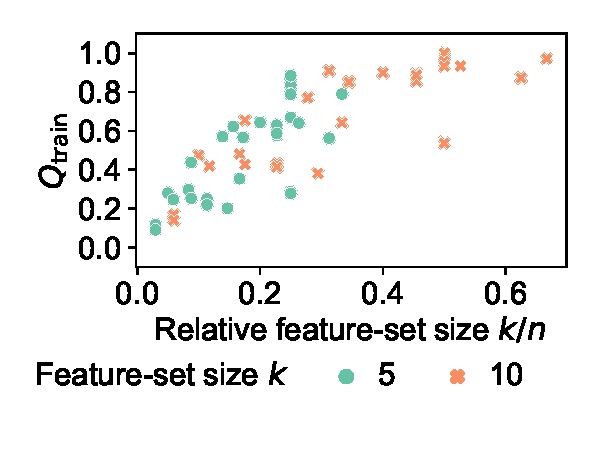
\includegraphics[width=\textwidth, trim=15 30 15 15, clip]{plots/afs-impact-dataset-k-train-objective.pdf}
		\caption{Training-set objective value.}
		\label{fig:afs:impact-dataset-k-train-objective}
	\end{subfigure}
	\hfill
	\begin{subfigure}[t]{0.48\textwidth}
		\centering
		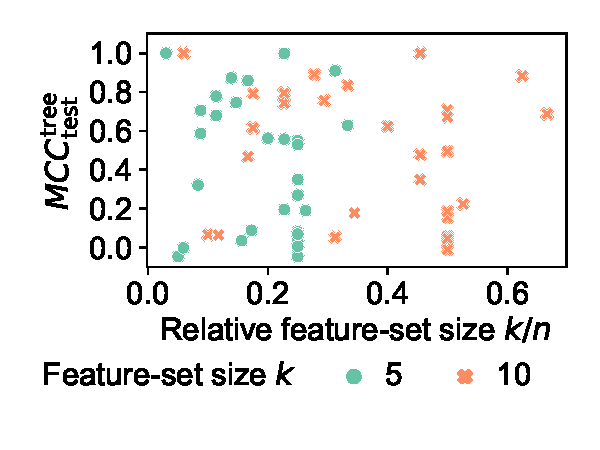
\includegraphics[width=\textwidth, trim=15 30 15 15, clip]{plots/afs-impact-dataset-k-decision-tree-test-mcc.pdf}
		\caption{Test-set prediction performance.}
		\label{fig:afs:impact-dataset-k-decision-tree-test-mcc}
	\end{subfigure}
	\caption{
		Feature-set quality over feature-set size~$k$ relative to dataset dimensionality~$n$.
		Results from the original feature sets of sequential search with \emph{MI} as feature-selection method.
	}
	\label{fig:afs:impact-dataset-k-quality}
\end{figure}

Naturally, feature-set quality depends on the datasets used, and several effects could occur.
For example, the distribution of feature-set quality in the datasets might be relatively uniform or relatively skewed.
Datasets with more features $n$ give way to more alternative feature sets.
At the same time, the feature quality can be spread over more features than for smaller datasets, making it harder to compose a small high-quality feature set.

Indeed, our experiments show a broad variation of feature-set quality over the datasets.
Figure~\ref{fig:afs:impact-dataset-k-quality} depicts the relationship between datasets and quality of the original feature set in sequential search.
To account for the varying number of features in the dataset, we put the ratio between feature-set size~$k$ and dataset dimensionality~$n$ on the x-axis, which is a measure of relative feature-set sizes.
As Figure~\ref{fig:afs:impact-dataset-k-train-objective} displays, the objective of an univariate feature-selection method approximately increases linearly with~$k/n$.
However, there still is some variation exclusively caused by the dataset rather than its dimensionality.
Further, the quality of a prediction model, i.e., decision trees, does not exhibit any trend but varies strongly between datasets, as Figure~\ref{fig:afs:impact-dataset-k-decision-tree-test-mcc} visualizes.
Due to this variance caused by dataset choice, we additionally normalize feature-set quality in some of the following analyses.
In particular, this normalization should reduce the influence of datasets and highlight the impact of other experimental settings instead.

\subsection{Feature-Set Quality Metrics}
\label{sec:afs:evaluation:metrics}

\begin{figure}[htb]
	\centering
	\begin{subfigure}[t]{0.48\textwidth}
		\centering
		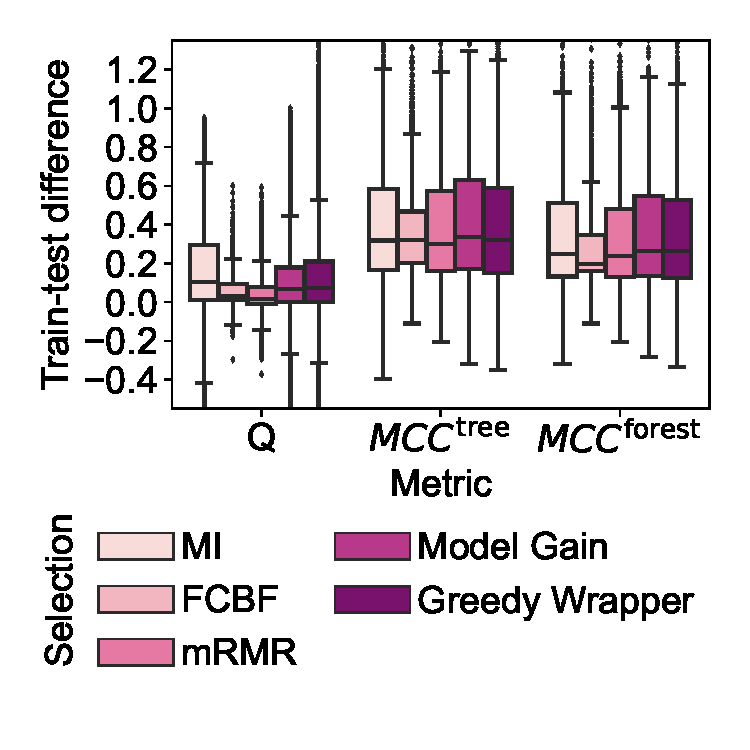
\includegraphics[width=\textwidth, trim=15 15 15 15, clip]{plots/afs-evaluation-metrics-overfitting.pdf}
		\caption{
			Training-test difference in feature-set quality by evaluation metric and feature-selection method.
			Y-axis truncated to improve readability.
		}
		\label{fig:afs:evaluation-metrics-overfitting}
	\end{subfigure}
	\hfill
	\begin{subfigure}[t]{0.48\textwidth}
		\centering
		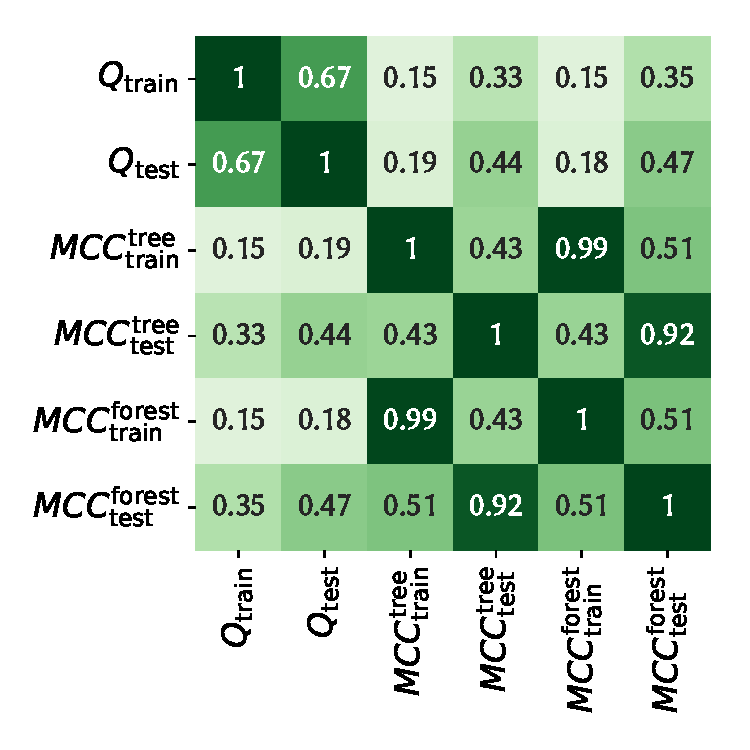
\includegraphics[width=\textwidth, trim=15 15 15 15, clip]{plots/afs-evaluation-metrics-correlation.pdf}
		\caption{Correlation between evaluation metrics, each calculated on the training set and the test set.}
		\label{fig:afs:evaluation-metrics-correlation}
	\end{subfigure}
	\caption{
		Feature-set quality by evaluation metric.
		Results from all search runs.
	}
	\label{fig:afs:evaluation-metrics}
\end{figure}

\paragraph{Prediction models and overfitting}

As one can expect, the average prediction performance of random forests is higher than that of decision trees.
Also, overfitting occurs for both model types, i.e., there is a gap between training-set and test-set prediction performance.
In particular, over all experimental settings, decision trees and random forests both have a mean training-set MCC of 0.85 (median: 1.0).
In contrast, on the test set, decision trees have a mean MCC of 0.48 (median: 0.54), while random forests have a slightly higher mean MCC of 0.52 (median: 0.63).
Thus, average prediction performance is significantly worse on the test set than on the training set.
When analyzing prediction performance in the following, we only report test-set performance.

For a more detailed comparison, Figure~\ref{fig:afs:evaluation-metrics-overfitting} shows the distribution of the difference between training and test feature-set quality, again over all experimental settings.
Once more, we observe that training feature-set quality is usually higher, i.e., the difference displayed in the figure is greater than zero.
Nevertheless, there are a few cases where the difference becomes negative, i.e., test feature-set quality is higher.
The existence of overfitting makes sense as we do not regularize, i.e., limit the growth of, the trees or prune them after training.
However, this does not invalidate our analysis of how prediction performance develops over alternatives.
The optimization objective~$Q$, which Figure~\ref{fig:afs:evaluation-metrics-overfitting} also depicts, shows overfitting for all feature-selection methods as well, though to a lesser extent than for prediction performance, so we consider training set and test set for this evaluation metric in the following.

\paragraph{Correlation between evaluation metrics}

Figure~\ref{fig:afs:evaluation-metrics-correlation} shows the Spearman correlation between different evaluation metrics over all experimental settings.
As the performance of decision trees and random forests is highly correlated on the training set as well as the test set, we only report prediction performance of one model in the following:
We choose decision trees, as they always consider all features during training, while random forests involve random sampling of features.

Figure~\ref{fig:afs:evaluation-metrics-correlation} also shows that the correlation between training and test feature-set quality is strong for the optimization objective~$Q$ and moderate for prediction performance in terms of MCC, but not very strong in either case.
This might be caused by different degrees of overfitting, depending on the experimental settings.
Further, the correlation between optimization objective~$Q$ and prediction MCC is only weak.
I.e., the objective of feature selection is only partially indicative of prediction performance since the former might use a simplified quality criterion.

\subsection{Feature-Selection Methods}
\label{sec:afs:evaluation:feature-selection}

\begin{figure}[htb]
	\centering
	\begin{subfigure}[t]{0.48\textwidth}
		\centering
		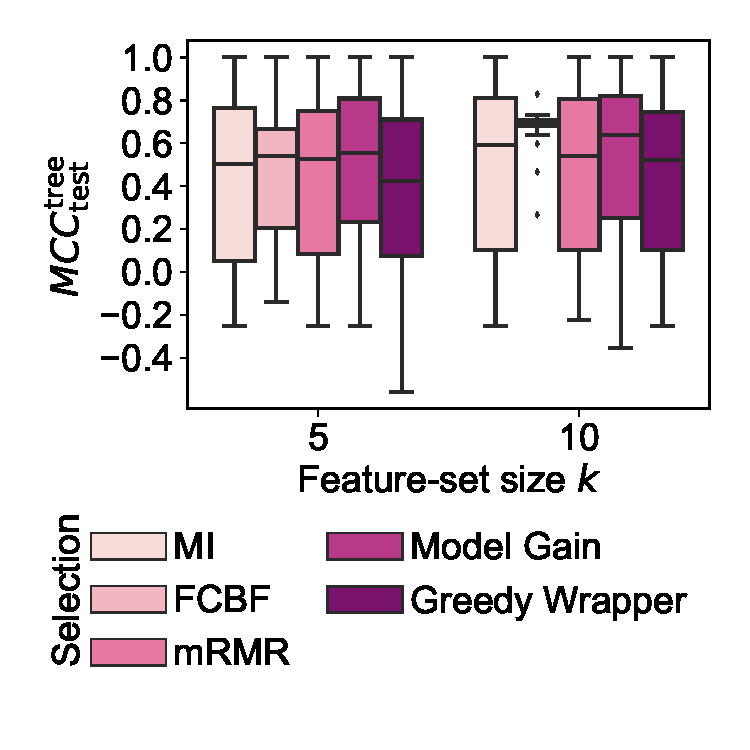
\includegraphics[width=\textwidth, trim=15 40 15 15, clip]{plots/afs-impact-fs-method-k-decision-tree-test-mcc.pdf}
		\caption{Test-set prediction performance.}
		\label{fig:afs:impact-fs-method-k-decision-tree-test-mcc}
	\end{subfigure}
	\hfill
	\begin{subfigure}[t]{0.48\textwidth}
		\centering
		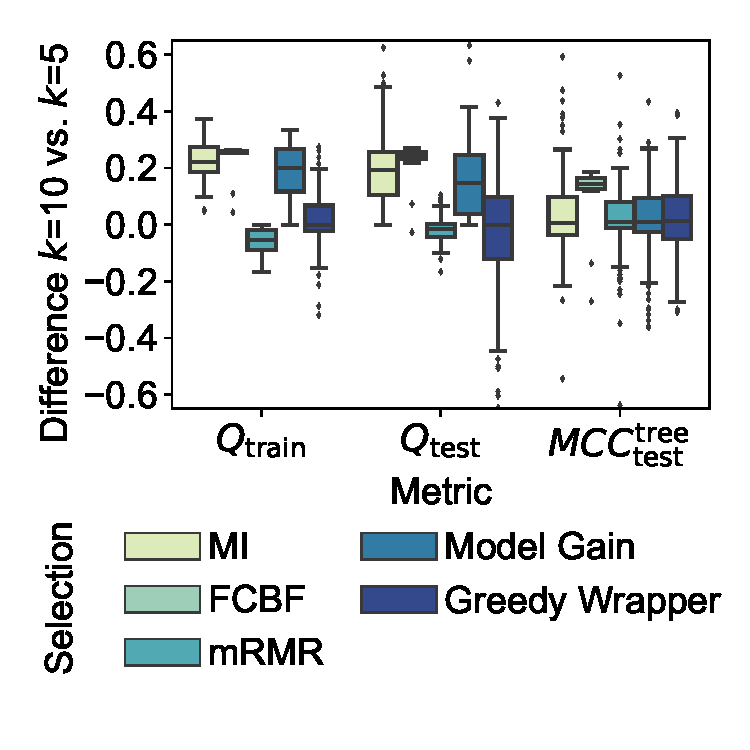
\includegraphics[width=\textwidth, trim=15 40 15 15, clip]{plots/afs-impact-fs-method-k-metric-diff.pdf}
		\caption{
			Difference in feature-set quality between $k=10$ and $k=5$ by evaluation metric.
			Y-axis truncated to improve readability.
		}
		\label{fig:afs:impact-fs-method-k-metric-diff}
	\end{subfigure}
	\caption{
		Feature-set quality by feature-selection method and feature-set size~$k$.
		Results from the original feature sets of sequential search.
	}
	\label{fig:afs:impact-fs-method-k-quality}
\end{figure}

\paragraph{Prediction performance}

As the different feature-selection methods employ different objective functions~$Q$, it does not make sense to compare absolute objective values between feature-selection methods to judge which method is best.
However, we can compare how useful the obtained feature sets are for predictions.
Figure~\ref{fig:afs:impact-fs-method-k-decision-tree-test-mcc} compares a decision tree's test-set prediction performance on the original feature sets of sequential search for different feature-selection methods.
On average, \emph{Model Gain} is the best feature-selection method, though not clearly better than the other feature-selection methods.
In particular, the median test-set MCC of decision trees is 0.59 for \emph{Model Gain}, 0.57 for \emph{FCBF}, and 0.54 for \emph{MI}, 0.53 for \emph{mRMR}, and 0.46 for \emph{Greedy Wrapper}.
In particular, the univariate, model-free feature scoring with \emph{MI} keeps up surprisingly well with the more sophisticated methods.
Thus, we focus on \emph{MI} for subsequent analyses of alternative feature sets, while still discussing the remaining feature-selection methods.
The overall best feature-selection method, \emph{Model Gain}, uses the same objective function as \emph{MI} but obtains its feature qualities from a prediction model rather than a bivariate dependency measure, which might be the crucial factor for its out-performance. 

The relatively bad performance of \emph{Greedy Wrapper} might result from its heuristic nature:
The wrapper search can only evaluate a fraction of all feasible feature sets and might get stuck in local optima, while the remaining feature-selection methods optimize globally.
In particular, \emph{Greedy Wrapper} only performed 71 iterations on average (median: 50) to determine the original feature sets of sequential search.
The figures concerning all experimental settings are similar, with a mean of 65 and a median of 45.
Thus, \emph{Greedy Wrapper} usually stayed significantly below the 1000~iterations we granted it.

Further, the results for \emph{FCBF} have to be taken with a grain of salt:
Over all experimental settings, 89\% of feature sets for \emph{FCBF} were infeasible, i.e., no feature set could satisfy the constraints.
In contrast, this figure only is 18\% for \emph{MI}.
Even the original feature set in sequential search is infeasible in 76\% of the cases for \emph{FCBF} but never for the other feature-selection methods.
In particular, the combination of feature-correlation constraints in our formulation of \emph{FCBF} (c.f.~Equation~\ref{eq:afs:fcbf}) with a feature-set-cardinality constraint, i.e., enforcing a certain feature-set size~$k$, seemingly made it hard to find valid feature sets.
This phenomenon becomes even more relevant the higher~$k$ is.

\paragraph{Influence of feature-set size~$k$}

As one can expect, larger feature sets, i.e., with~$k=10$, usually exhibit higher feature-set quality than smaller feature sets, i.e., with $k=5$.
However, the increase in feature-set quality with $k$ is not proportional, and there might even be a decrease.
As Figure~\ref{fig:afs:impact-fs-method-k-metric-diff} shows for the original feature sets of sequential search, \emph{MI}, \emph{FBCF}, and \emph{Model Gain} exhibit a slight increase of the training-set objective value~$Q_\text{train}$ from~$k=5$ to~$k=10$, i.e., the difference depicted in Figure~\ref{fig:afs:impact-fs-method-k-metric-diff} is positive.
As these objectives are monotonic in the set of selected features, a decrease in training-set quality is not possible.
In contrast, the heuristic \emph{Greedy Wrapper} does not necessarily benefit from selecting more features.
The latter insight applies to the white-box method \emph{mRMR} as well since it normalizes its objective with the number of selected features and penalizes feature redundancy.
As Figure~\ref{fig:afs:impact-fs-method-k-metric-diff} also displays, the benefit of larger feature sets is even less clear for prediction performance.
In particular, all feature-selection methods except \emph{FCBF} show a median difference in test-set MCC close to zero when comparing $k=5$ to $k=10$.
Thus, we focus on smaller feature sets, i.e., $k=5$, in the following.

\subsection{Searching Alternatives}
\label{sec:afs:evaluation:search}

In this section, we evaluate the different choices for searching alternatives: the search method (cf.~Section~\ref{sec:afs:evaluation:search:method}), number of alternatives~$a$ (cf.~Section~\ref{sec:afs:evaluation:search:num-alternatives}), and dissimilarity threshold~$\tau$ (cf.~Section~\ref{sec:afs:evaluation:search:tau}).

\subsubsection{Search Method}
\label{sec:afs:evaluation:search:method}

\begin{figure}[p]
	\centering
	\begin{subfigure}[t]{0.48\textwidth}
		\centering
		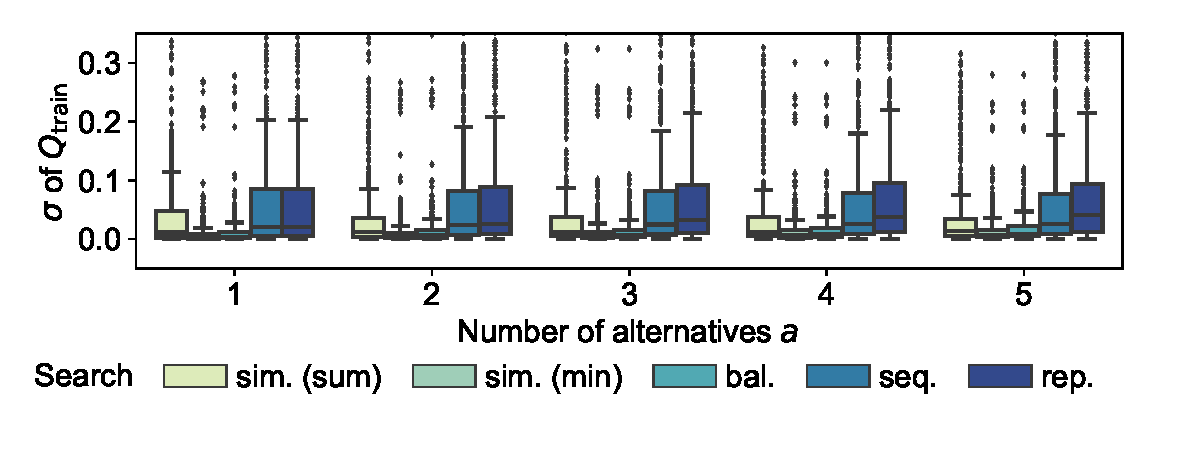
\includegraphics[width=\textwidth, trim=15 25 15 10, clip]{plots/afs-impact-search-stddev-train-objective.pdf}
		\caption{Standard deviation of training-set objective value within search runs.}
		\label{fig:afs:impact-search-stddev-train-objective}
	\end{subfigure}
	\hfill
	\begin{subfigure}[t]{0.48\textwidth}
		\centering
		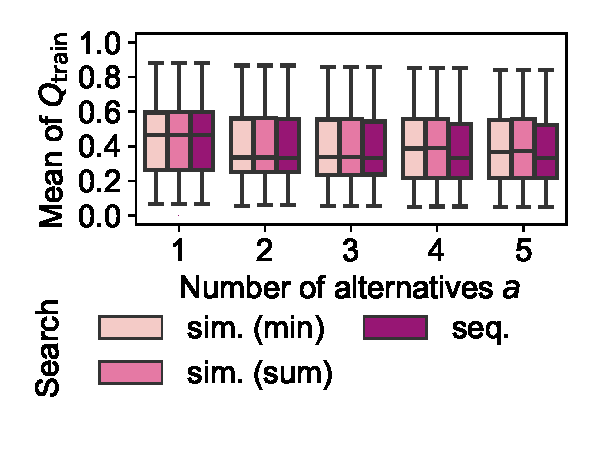
\includegraphics[width=\textwidth, trim=15 25 15 10, clip]{plots/afs-impact-search-mean-train-objective.pdf}
		\caption{Mean of training-set objective value within search runs.}
		\label{fig:afs:impact-search-mean-train-objective}
	\end{subfigure}
	\\ \vspace{\baselineskip}
	\begin{subfigure}[t]{0.48\textwidth}
		\centering
		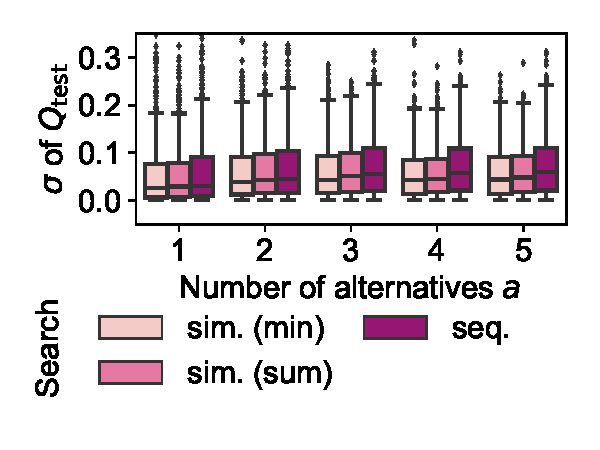
\includegraphics[width=\textwidth, trim=15 25 15 15, clip]{plots/afs-impact-search-stddev-test-objective.pdf}
		\caption{Standard deviation of test-set objective value within search runs.}
		\label{fig:afs:impact-search-stddev-test-objective}
	\end{subfigure}
	\hfill
	\begin{subfigure}[t]{0.48\textwidth}
		\centering
		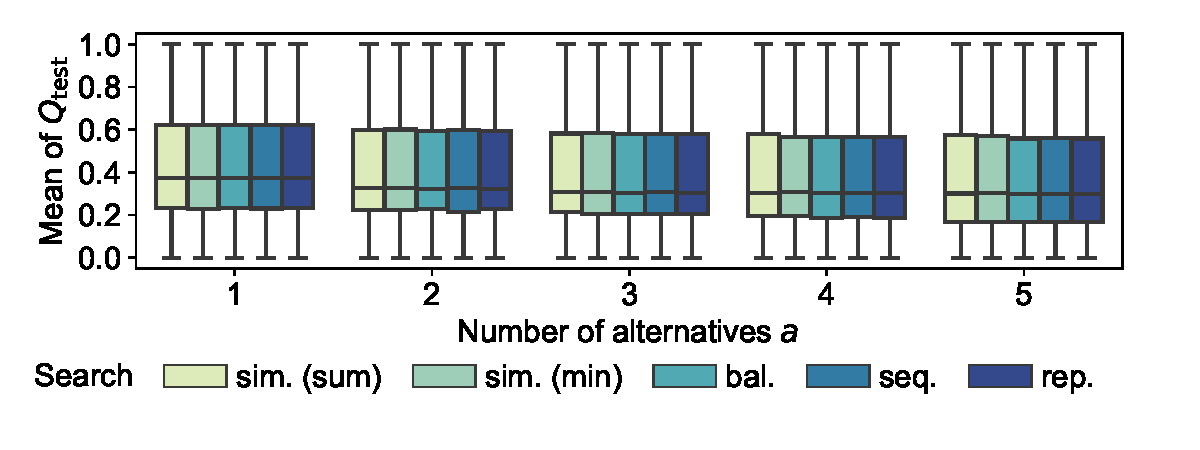
\includegraphics[width=\textwidth, trim=15 25 15 15, clip]{plots/afs-impact-search-mean-test-objective.pdf}
		\caption{Mean of test-set objective value with\-in search runs.}
		\label{fig:afs:impact-search-mean-test-objective}
	\end{subfigure}
	\\ \vspace{\baselineskip}
	\begin{subfigure}[t]{0.48\textwidth}
		\centering
		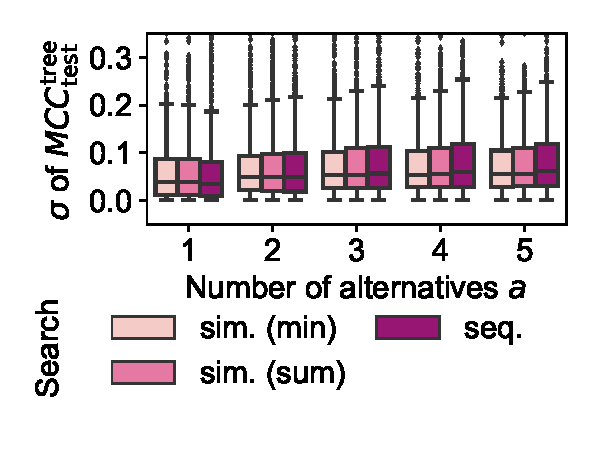
\includegraphics[width=\textwidth, trim=15 25 15 5, clip]{plots/afs-impact-search-stddev-decision-tree-test-mcc.pdf}
		\caption{Standard deviation of test-set prediction performance within search runs.}
		\label{fig:afs:impact-search-stddev-decision-tree-test-mcc}
	\end{subfigure}
	\hfill
	\begin{subfigure}[t]{0.48\textwidth}
		\centering
		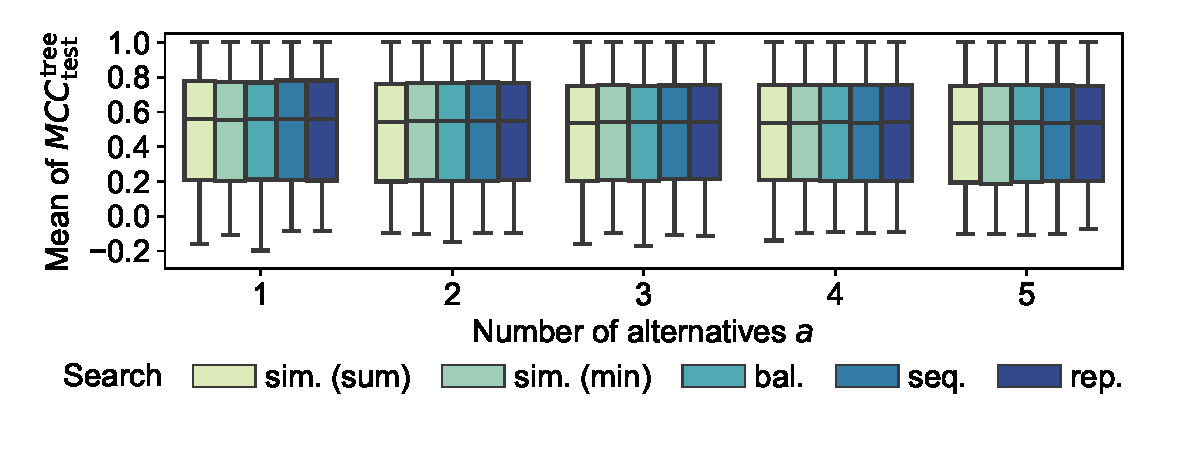
\includegraphics[width=\textwidth, trim=15 25 15 5, clip]{plots/afs-impact-search-mean-decision-tree-test-mcc.pdf}
		\caption{Mean of test-set prediction performance within search runs.}
		\label{fig:afs:impact-search-mean-decision-tree-test-mcc}
	\end{subfigure}
	\caption{
		Feature-set quality over the number of alternatives, by evaluation metric and search method for alternatives.
		Results with \emph{MI} as feature-selection method and $k=5$.
		Y-axes truncated to improve readability.
	}
	\label{fig:afs:impact-search-quality}
\end{figure}

\begin{figure}[htb]
	\centering
	\begin{subfigure}[t]{0.48\textwidth}
		\centering
		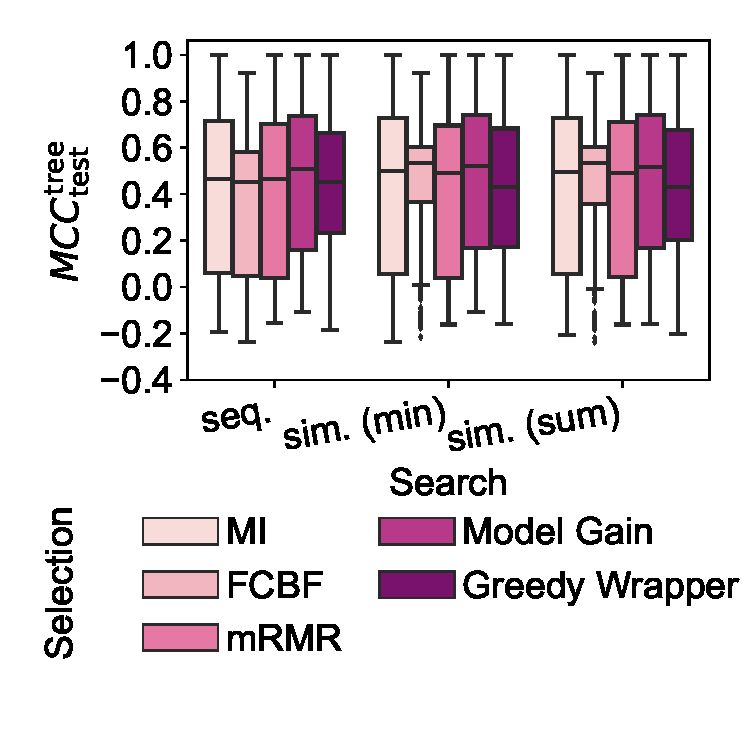
\includegraphics[width=\textwidth, trim=15 40 15 10, clip]{plots/afs-impact-search-fs-method-decision-tree-test-mcc.pdf}
		\caption{Test-set prediction performance.}
		\label{fig:afs:impact-search-fs-method-decision-tree-test-mcc}
	\end{subfigure}
	\hfill
	\begin{subfigure}[t]{0.48\textwidth}
		\centering
		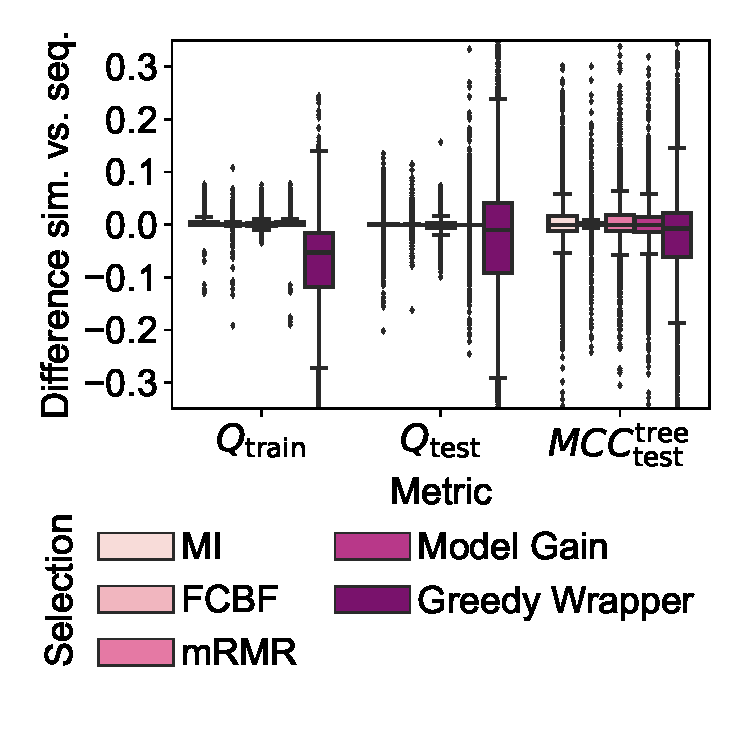
\includegraphics[width=\textwidth, trim=15 40 15 10, clip]{plots/afs-impact-search-fs-method-metric-diff.pdf}
		\caption{
			Difference in feature-set quality between simultaneous (summed-quality) and sequential search by evaluation metric.
			Y-axis truncated to improve readability.
		}
		\label{fig:afs:impact-search-fs-method-metric-diff}
	\end{subfigure}
	\caption{
		Feature-set quality by feature-selection method and search method for alternatives.
		Results with $k=5$ and up to five alternatives.
	}
	\label{fig:afs:impact-search-fs-method-quality}
\end{figure}

\paragraph{Variance in feature-set quality}

As expected, the choice of the search method influences how much the training-set objective value~$Q$ varies between alternatives found within each search run.
Figure~\ref{fig:afs:impact-search-stddev-train-objective} visualizes this observation for \emph{MI} as feature-selection method and $k=5$.
In particular, multiple alternative feature sets found by sequential search usually vary more in their quality than for simultaneous search.
When using simultaneous search, the minimum-quality objective yields significantly more homogeneous feature-set quality than the summed-quality objective.
These findings apply to all white-box feature-selection methods but not the heuristic \emph{Greedy Wrapper}.

As Figures~\ref{fig:afs:impact-search-stddev-test-objective} and~\ref{fig:afs:impact-search-stddev-decision-tree-test-mcc} show, the difference between the search methods is clearly less prominent when observing the variance of feature-set quality on the test set.
This observation applies to quality in terms of objective value as well as prediction performance.
In particular, alternatives found by simultaneous search do not have considerably more homogeneous test feature-set quality than for sequential search.
This effect might be a result of overfitting:
Even if training feature-set quality is similar, some alternatives might generalize better, i.e., maintain their quality on the test set, while other alternatives might loose quality to a larger extent.
Thus, the variance in test feature-set quality caused by overfitting could alleviate the effect on variance caused by the search method.

\paragraph{Average value of feature-set quality}

While obtaining alternatives of more homogeneous quality can be one goal of simultaneous search, the main selling point would be obtaining alternatives of higher average quality.
However, we found that simultaneous search is not clearly better than sequential search in that regard.
In particular, Figure~\ref{fig:afs:impact-search-mean-train-objective} compares the distribution of the mean training-set objective in search runs for \emph{MI} as feature-selection method and $k=5$.
We observe that all search methods yield very similar distribution of training-set objective values.
This observation holds for all four white-box feature selection methods, while the heuristic \emph{Greedy Wrapper} even favors sequential search over simultaneous search.
In contrast, for \emph{MI}, as visible in Figure~\ref{fig:afs:impact-search-mean-train-objective}, and \emph{Model Gain}, simultaneous search tends to develop a slight advantage over sequential search at least with a growing number of alternatives.

The negligible quality difference between the search methods is also visible for the test-set objective value in Figure~\ref{fig:afs:impact-search-mean-test-objective} and the test-set prediction performance in Figure~\ref{fig:afs:impact-search-mean-decision-tree-test-mcc}.
In particular, as Figure~\ref{fig:afs:impact-search-fs-method-decision-tree-test-mcc} displays, other aspects of the experimental design, e.g., dataset, dissimilarity threshold~$\tau$, etc. cause a larger variation in prediction performance, which exceeds the variation between the search methods.

As a final quality comparison, Figure~\ref{fig:afs:impact-search-fs-method-metric-diff} displays the difference in feature-set quality between sequential and simultaneous search if it is compared on each search setting separately, i.e., each combination of dataset, fold, dissimilarity threshold~$\tau$, etc.
The figure again shows that all feature-selection methods except \emph{Greedy Wrapper} exhibit little variation in quality between these two search approaches, apart from some outlying experimental settings, i.e., the difference in feature-set quality is usually close to zero.
Additionally, the figure highlights that outliers can occur in both directions:
While simultaneous search can yield better-performing feature sets in some situations, sequential search can be significantly better in other scenarios.

\begin{table}[htb]
	\centering
	\begin{tabular}{llrrrr}
		\toprule
		Selection & Search & \multicolumn{4}{c}{Optimization status} \\
		\cmidrule(r){3-6}
		& & Infeasible & Not solved & Feasible & Optimal \\
		\midrule
		FCBF & seq. & 70.25\% & 0.00\% & 0.00\% & 29.75\% \\
		FCBF & sim. (min) & 74.13\% & 0.08\% & 1.45\% & 24.33\% \\
		FCBF & sim. (sum) & 74.12\% & 0.09\% & 2.01\% & 23.77\% \\
		MI & seq. & 1.97\% & 0.00\% & 0.00\% & 98.03\% \\
		MI & sim. (min) & 4.67\% & 0.00\% & 8.80\% & 86.53\% \\
		MI & sim. (sum) & 4.67\% & 0.00\% & 2.44\% & 92.89\% \\
		Model Gain & seq. & 1.97\% & 0.00\% & 0.00\% & 98.03\% \\
		Model Gain & sim. (min) & 4.67\% & 0.00\% & 5.25\% & 90.08\% \\
		Model Gain & sim. (sum) & 4.67\% & 0.00\% & 1.75\% & 93.59\% \\
		mRMR & seq. & 1.96\% & 0.00\% & 9.90\% & 88.14\% \\
		mRMR & sim. (min) & 4.67\% & 0.00\% & 48.72\% & 46.61\% \\
		mRMR & sim. (sum) & 4.67\% & 0.00\% & 66.99\% & 28.35\% \\
		\bottomrule
	\end{tabular}
	\caption{
		Frequency of optimization statuses (cf.~Section~\ref{sec:afs:experimental-design:evaluation}) by feature-selection method and search method for alternatives.
		Results with $k=5$ and up to five alternatives.
		Excluding \emph{Greedy Wrapper}, which calls the solver multiple times, and checks satisfiability rather than optimizing.
		Each row sums to 100\%.
	}
	\label{tab:afs:impact-search-fs-method-optimization-status}
\end{table}
%
\begin{table}[htb]
	\centering
	\begin{tabular}{rrrrr}
		\toprule
		$a$ & \multicolumn{4}{c}{Optimization status} \\
		\cmidrule(r){2-5}
		& Infeasible & Not solved & Feasible & Optimal \\
		\midrule
		1 & 16.88\% & 0.00\% & 7.45\% & 75.67\% \\
		2 & 17.97\% & 0.00\% & 13.63\% & 68.40\% \\
		3 & 20.20\% & 0.00\% & 20.03\% & 59.77\% \\
		4 & 26.90\% & 0.02\% & 21.42\% & 51.67\% \\
		5 & 28.20\% & 0.10\% & 28.95\% & 42.75\% \\
		\bottomrule
	\end{tabular}
	\caption{
		Frequency of optimization statuses (cf.~Section~\ref{sec:afs:experimental-design:evaluation}) by number of alternatives~$a$.
		Results from simultaneous search with summed-quality objective and $k=5$, excluding \emph{Greedy Wrapper} as feature-selection method.
		Each row sums to 100\%.
	}
	\label{tab:afs:impact-num-alternatives-optimization-status}
\end{table}

\paragraph{Optimization status}

A major reason for simultaneous search failing to consistently beat sequential search quality-wise is that search results can be sub-optimal.
For \emph{Greedy Wrapper}, the search is heuristic per se, and only a tiny fraction of the search space is covered.
For the four white-box feature-selection methods, the solver can time out.
As the optimization problem of simultaneous search is harder than for sequential search (cf.~Table~\ref{tab:afs:seq-sim-comparison}), it has a higher likelihood to run into timeouts.
Table~\ref{tab:afs:impact-search-fs-method-optimization-status} visualizes this phenomenon.
In particular, for up to five alternatives and $k=5$, all sequential searches for \emph{FCBF}, \emph{MI}, and \emph{Model Gain} finished within the timeout, i.e., yielded the optimal feature set or ascertained infeasibility.
For \emph{mRMR}, there are about 10\% potentially suboptimal feature sets under the same settings.
In contrast, for simultaneous search with the summed-quality objective, all feature-selection methods experience timeouts in searches:
Roughly 2\% of the searches for \emph{FCBF}, \emph{MI}, and \emph{Model Gain}, and 67\% of the searches for \emph{mRMR} found a feasible solution till the timeout but could not guarantee optimality.
Such timeout-affected solutions of simultaneous search can be worse than an optimal sequential solution.
With the minimum-quality objective instead of the summed-quality objective in simultaneous search, the number of timeouts increases for \emph{MI} and \emph{Model Gain} but decreases for \emph{FCBF} and \emph{mRMR}.
Still, sequential search runs into less timeouts for all four white-box feature-selection methods.

Besides finding suboptimal feature sets, the solver might also fail to find a feasible solution without being able to guarantee infeasibility.
However, this optimization status, called \emph{not solved}, occurred rarely in our experiments, and only for \emph{FCBF} in simultaneous search.
Further, note that the fraction of timeouts strongly depends on the number of alternatives~$a$, as Table~\ref{tab:afs:impact-num-alternatives-optimization-status} displays:
For simultaneous search with $k=5$ and the summed-quality objective, roughly 7\% of the white-box searches timed out for one alternative but 20\% for three alternatives and 29\% for five alternatives.
Remember that we grant simultaneous searches proportionally more time to obtain more feature sets.
The nevertheless observed increase in timeouts suggests that runtime increases super-proportionally, as we analyze next.

\begin{table}[htb]
	\centering
	\begin{tabular}{lrrr}
		\toprule
		Selection & \multicolumn{3}{c}{Optimization time} \\
		\cmidrule(r){2-4}
		& seq. & sim. (min) & sim. (sum) \\
		\midrule
		FCBF & 0.02~s & 0.14~s & 0.12~s \\
		Greedy Wrapper & 3.46~s & 3.09~s & 3.28~s \\
		MI & 0.02~s & 1.25~s & 0.15~s \\
		Model Gain & 0.02~s & 0.82~s & 0.13~s \\
		mRMR & 2.80~s & 120.00~s & 239.69~s \\
		\bottomrule
	\end{tabular}
	\caption{
		Median optimization time by feature-selection method and search method for alternatives.
		Results with $k=5$ and up to five alternatives.
	}
	\label{tab:afs:impact-search-fs-method-optimization-time}
\end{table}
%
\begin{table}[htb]
	\centering
	\begin{tabular}{lrrrrr}
		\toprule
		$a$ & \multicolumn{5}{c}{Optimization time} \\
		\cmidrule(r){2-6}
		& FCBF & Wrapper & MI & Model Gain & mRMR \\
		\midrule
		1 & 0.04~s & 1.61~s & 0.01~s & 0.01~s & 12.09~s \\
		2 & 0.07~s & 2.47~s & 0.05~s & 0.05~s & 179.85~s \\
		3 & 0.13~s & 3.29~s & 0.20~s & 0.17~s & 239.93~s \\
		4 & 0.21~s & 5.31~s & 1.75~s & 1.44~s & 299.91~s \\
		5 & 0.28~s & 7.26~s & 61.34~s & 30.09~s & 359.91~s \\
		\bottomrule
	\end{tabular}
	\caption{
		Median optimization time by feature-selection method and number of alternatives~$a$.
		Results from simultaneous search with summed-quality objective and $k=5$.
	}
	\label{tab:afs:impact-num-alternatives-fs-method-optimization-time}
\end{table}

\paragraph{Optimization time}

Analyzing the actual optimization time instead of the optimization status also speaks in favor of sequential search.
As Table~\ref{tab:afs:impact-search-fs-method-optimization-time} shows, the median optimization time of sequential search is lower for all five feature-selection methods.
In particular, the difference in median optimization time between sequential and simultaneous search is one to two orders of magnitude for the four white-box feature-selection methods.
Further, \emph{MI}, and \emph{Model Gain} experiences a dramatic, clearly super-linear increase in median optimization time with the number of alternatives~$a$ in simultaneous search, as Table~\ref{tab:afs:impact-num-alternatives-fs-method-optimization-time} displays.
In contrast, the runtime increase is considerably less for sequential search since it shows an approximately linear trend with the number of alternatives there.

Based on all results described in this section, we focus on the sequential search in the following.
In particular, it appeared to be significantly faster than simultaneous search while yielding similar feature-set quality.

Another interesting question for practitioners is how the runtime relates to~$n$, the total number of features in the dataset.
One would expect a positive correlation, since the optimization problem's instance size increases with~$n$.
Roughly speaking, this trend also appears in our experimental data.
However, the observed trend does not match a simple functional relationship, and some higher-dimensional datasets even show lower average runtimes than lower-dimensional datasets.
This indicates that several other factors apart from~$n$ influence solver runtime.
Besides factors related to our experimental design and the datasets, the heuristics employed by the solver might also play a role, e.g., work better for some problem instances than for others.

\subsubsection{Number of Alternatives \texorpdfstring{$a$}{}}
\label{sec:afs:evaluation:search:num-alternatives}

\begin{figure}[p]
	\centering
	\begin{subfigure}[t]{\textwidth}
		\centering
		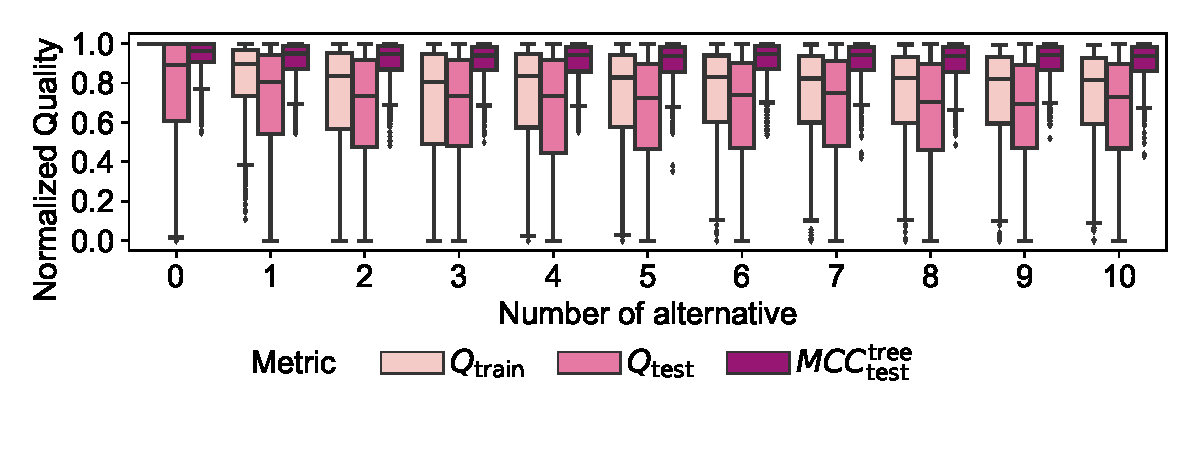
\includegraphics[width=\textwidth, trim=15 30 15 15, clip]{plots/afs-impact-num-alternatives-quality-max.pdf}
		\caption{Max-normalized, infeasible feature sets excluded.}
		\label{fig:afs:impact-num-alternatives-quality-max}
	\end{subfigure}
	\begin{subfigure}[t]{\textwidth}
		\centering
		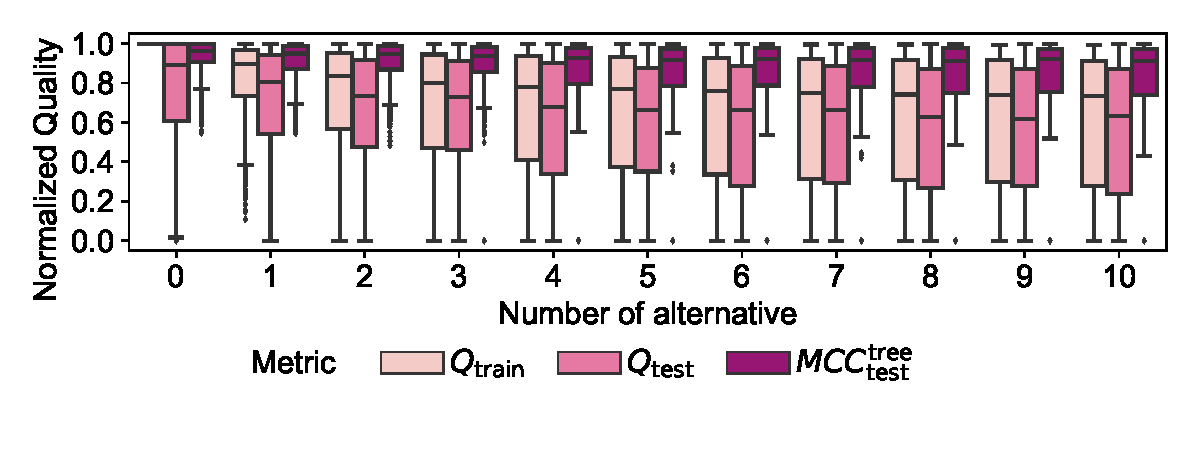
\includegraphics[width=\textwidth, trim=15 30 15 15, clip]{plots/afs-impact-num-alternatives-quality-max-fillna.pdf}
		\caption{Max-normalized, infeasible feature sets assigned a quality of~0.}
		\label{fig:afs:impact-num-alternatives-quality-max-fillna}
	\end{subfigure}
	\begin{subfigure}[t]{\textwidth}
		\centering
		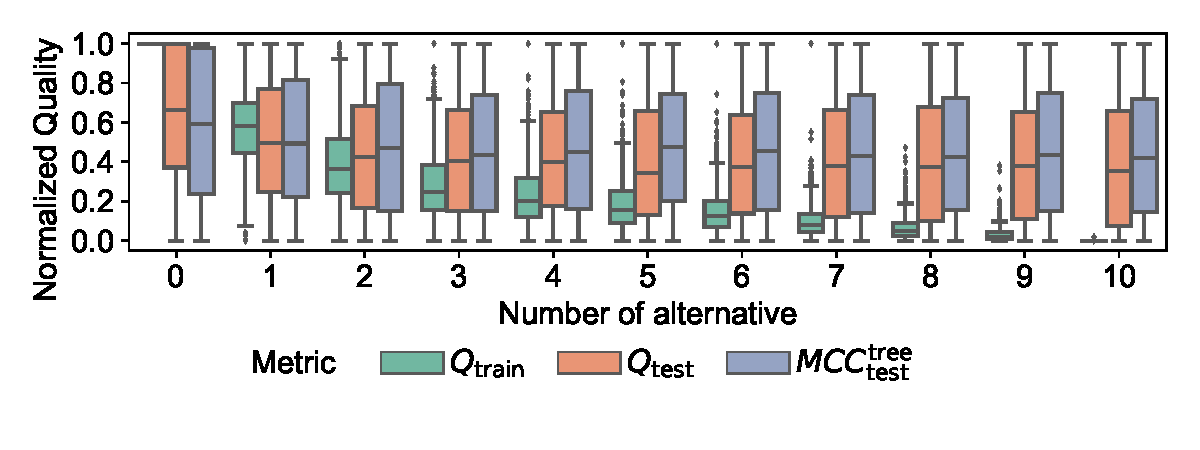
\includegraphics[width=\textwidth, trim=15 30 15 15, clip]{plots/afs-impact-num-alternatives-quality-min-max.pdf}
		\caption{Min-max-normalized, infeasible feature sets excluded.}
		\label{fig:afs:impact-num-alternatives-quality-min-max}
	\end{subfigure}
	\begin{subfigure}[t]{\textwidth}
		\centering
		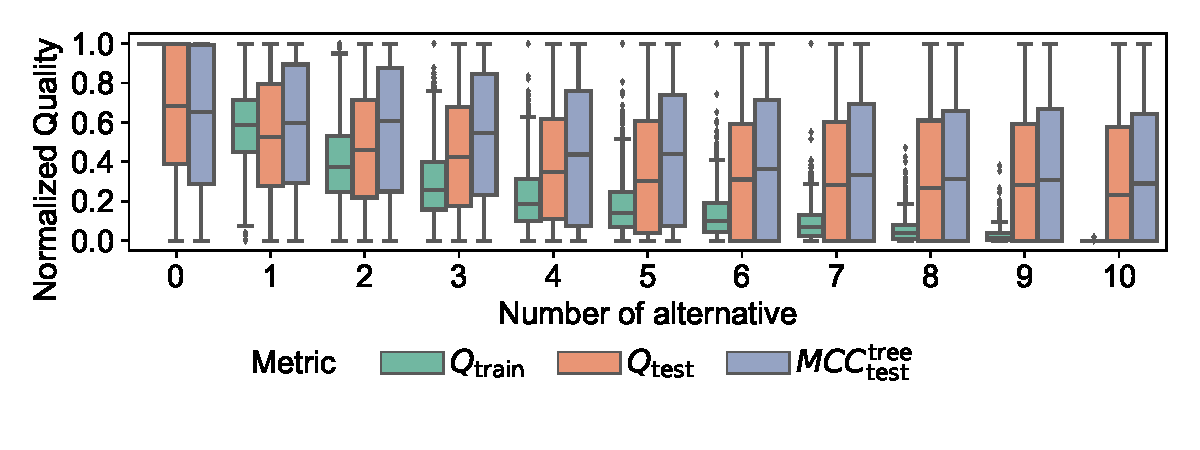
\includegraphics[width=\textwidth, trim=15 30 15 15, clip]{plots/afs-impact-num-alternatives-quality-min-max-fillna.pdf}
		\caption{Min-max-normalized, infeasible feature sets assigned a quality of~0.}
		\label{fig:afs:impact-num-alternatives-quality-min-max-fillna}
	\end{subfigure}
	\caption{
		Feature-set quality, normalized per experimental setting, over the number of alternatives, by evaluation metric.
		Results from sequential search with \emph{MI} as feature-selection method and $k=5$.
	}
	\label{fig:afs:impact-num-alternatives-quality}
\end{figure}

\paragraph{Feature-set quality}

For sequential search, the training-set objective value naturally decreases with the number of alternatives, at least for the feature-selection criteria optimized exactly.
In particular, each found feature set adds another constraint to the optimization problem.
Figures~\ref{fig:afs:impact-num-alternatives-quality-max} and~\ref{fig:afs:impact-num-alternatives-quality-min-max} illustrate this trend for \emph{MI}-based feature selection.
Since feature-set quality varies between datasets and cross-validation folds, as discussed in Section~\ref{sec:afs:evaluation:datasets}, we additionally normalize feature-set quality here.
In particular, we analyze the relative development of feature-set quality within individual search runs for alternatives.
First, we shift the range of all evaluation metrics to~$[0,1]$.
In particular, MCC to measure prediction performance as well as the objective value of \emph{Greedy Wrapper} and \emph{mRMR} would have the range~$[-1,1]$ without this shift.
Second, in Figure~\ref{fig:afs:impact-num-alternatives-quality-max}, we have max-normalized the feature-set quality for each search of alternatives, i.e., the highest feature-set quality in the search run is scaled to~1 and the other feature-set qualities are scaled accordingly.
This figure shows that there might be multiple alternatives of similar quality, as the median training-set objective value remains relatively stable over the number of alternatives.
In particular, the median training-set objective value remains relative close to the maximum of~1 and is above 0.8 even for the tenth alternative.
For comparison, Figure~\ref{fig:afs:impact-num-alternatives-quality-min-max} uses min-max normalization, i.e., the worst of the alternatives gets~0 as objective.
This figure makes the decrease in objective value over the number of alternatives more visible.
In particular, this figure highlights that the training-set objective value decreases most from the original feature set to the first alternative but less beyond.

Additionally, Figures~\ref{fig:afs:impact-num-alternatives-quality-max} and~\ref{fig:afs:impact-num-alternatives-quality-min-max} show that the test-set objective value also drops most from the original feature set to the first alternative.
However, the decrease in median test-set objective value over the alternatives only occurs for the first few alternatives.
For further alternatives, the median test-set objective value is stable.
Additionally, the initial decrease in quality is less prominent than on the training set.
In particular, alternatives can even have a higher test-set objective value than the original feature set due to overfitting.
Similar findings hold for test-set prediction performance.
Overall, these results indicate that alternative feature sets fulfill their purpose of being different solutions with similar quality as the original feature set.

\paragraph{Optimization status}

Be aware that these observations refer to the quality of the found feature sets.
However, the more alternatives are desired, the more likely an infeasible optimization problem is.
For example, the \emph{MI} feature-selection method in sequential search always finds an original feature set.
However, with $k=5$, the problem is infeasible in 2\% of the cases for the third alternative, 12\% for the fifth alternative, and 17\% for the tenth alternative.
Increasing the feature-set size $k$, e.g., to $k=10$, or decreasing the dataset dimensionality~$n$, naturally increases the number of infeasible solutions, as less features become available for alternatives.
Thus, while the quality of actually found feature sets seems to remain relatively stable with an increased number of alternatives, valid alternatives might simply not exist.
Figures~\ref{fig:afs:impact-num-alternatives-quality-max-fillna} and~\ref{fig:afs:impact-num-alternatives-quality-min-max-fillna} show the same data as Figures~\ref{fig:afs:impact-num-alternatives-quality-max} and~\ref{fig:afs:impact-num-alternatives-quality-min-max} except with the quality of infeasible feature sets set to zero, i.e., the theoretical minimum after we shifted the value ranges of all evaluation metrics.
In these figures, the downward trend of feature-set quality over the number of alternatives becomes slightly more prominent, particular for a high number of alternatives.
This downward trend also depends on the dissimilarity threshold~$\tau$, which we analyze in the next section.

\begin{figure}[htb]
	\centering
	\begin{subfigure}[t]{0.48\textwidth}
		\centering
		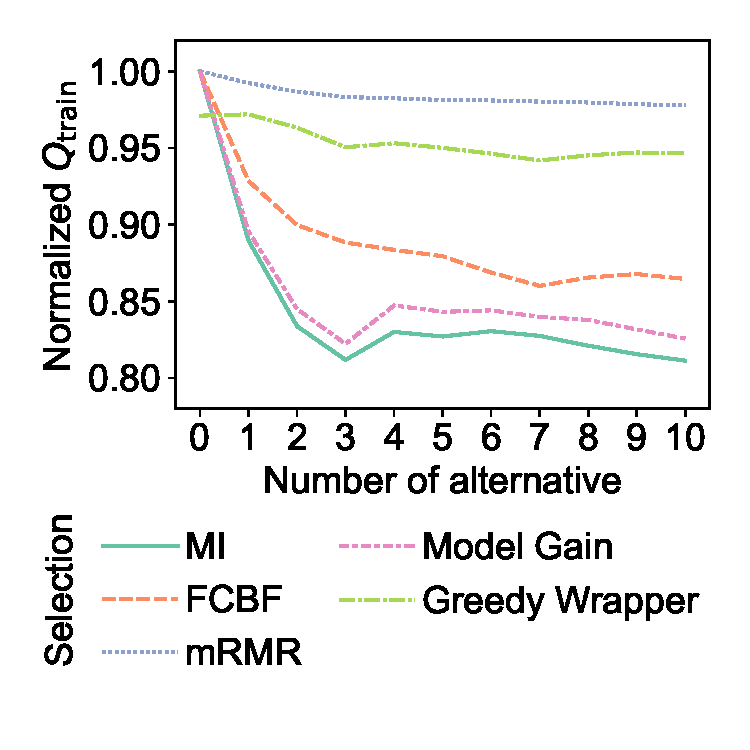
\includegraphics[width=\textwidth, trim=20 40 15 15, clip]{plots/afs-impact-num-alternatives-fs-method-train-objective-max.pdf}
		\caption{Training-set objective value.}
		\label{fig:afs:impact-num-alternatives-fs-method-train-objective-max}
	\end{subfigure}
	\hfill
	\begin{subfigure}[t]{0.48\textwidth}
		\centering
		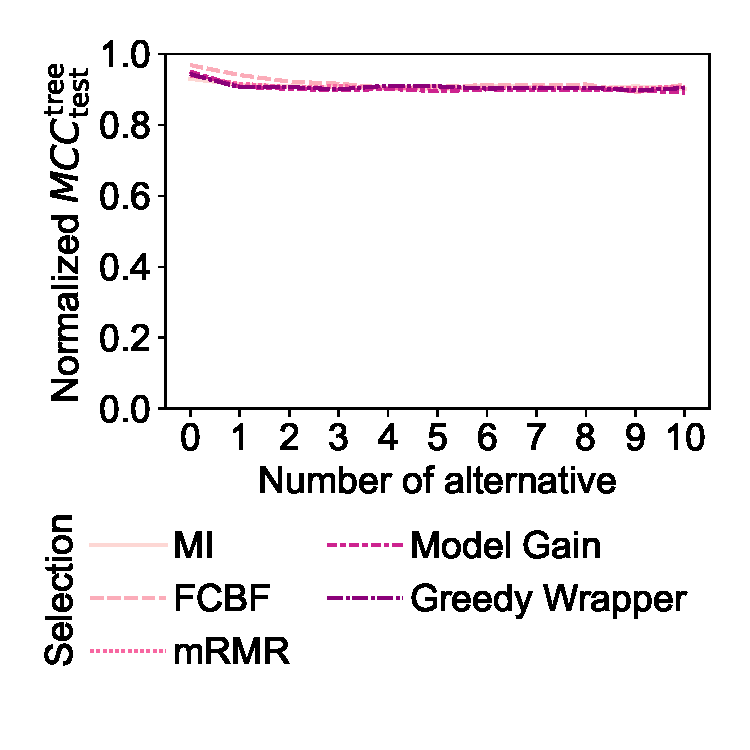
\includegraphics[width=\textwidth, trim=20 40 15 15, clip]{plots/afs-impact-num-alternatives-fs-method-decision-tree-test-mcc-max.pdf}
		\caption{Test-set prediction performance.}
		\label{fig:afs:impact-num-alternatives-fs-method-decision-tree-test-mcc-max}
	\end{subfigure}
	\caption{
		Median feature-set quality, max-normalized per experimental setting, over the number of alternatives, by evaluation metric.
		Infeasible feature sets excluded.
		Results from sequential search with $k=5$.
	}
	\label{fig:afs:impact-num-alternatives-fs-method-quality}
\end{figure}

\paragraph{Influence of feature-selection method}

While we discussed \emph{MI} before, the decrease of objective value over the number of alternatives occurs for all feature-selection methods in our experiments, as Figure~\ref{fig:afs:impact-num-alternatives-fs-method-train-objective-max} shows.
The strength of the decrease varies between the feature selection methods.
For example, \emph{Greedy Wrapper} and \emph{mRMR} show little effect of increasing the number alternatives.
Further, for the test-set prediction performance, displayed in Figure~\ref{fig:afs:impact-num-alternatives-fs-method-decision-tree-test-mcc-max} none of the feature-selection methods exhibits a strong decrease over the number of alternatives.

\subsubsection{Dissimilarity Threshold \texorpdfstring{$\tau$}{}} % \texorpdfstring prevents warning "Token not allowed in a PDF string"
\label{sec:afs:evaluation:search:tau}

\begin{figure}[p]
	\centering
	\begin{subfigure}[t]{0.48\textwidth}
		\centering
		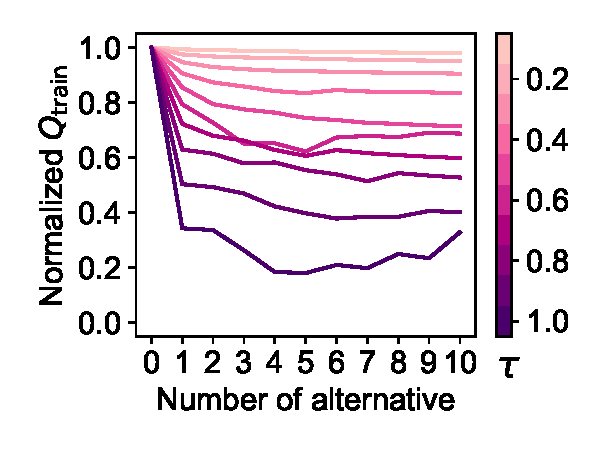
\includegraphics[width=\textwidth, trim=15 15 10 15, clip]{plots/afs-impact-num-alternatives-tau-train-objective-max.pdf}
		\caption{
			Training-set objective value, max-normalized.
			Infeasible feature sets excluded.
		}
		\label{fig:afs:impact-num-alternatives-tau-train-objective-max}
	\end{subfigure}
	\hfill
	\begin{subfigure}[t]{0.48\textwidth}
		\centering
		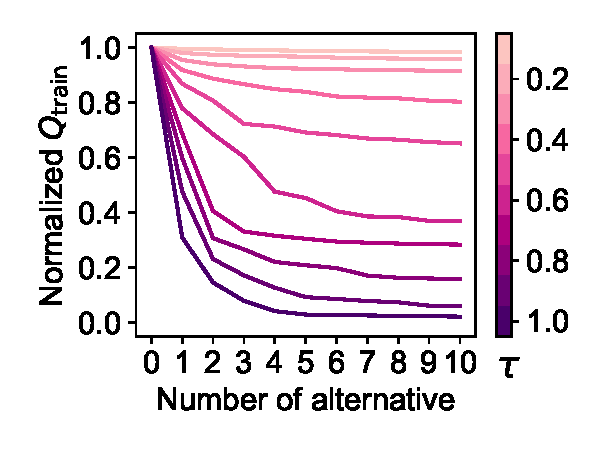
\includegraphics[width=\textwidth, trim=15 15 10 15, clip]{plots/afs-impact-num-alternatives-tau-train-objective-max-fillna.pdf}
		\caption{
			Training-set objective value, max-normalized.
			Infeasible feature sets assigned a quality of~0.
		}
		\label{fig:afs:impact-num-alternatives-tau-train-objective-max-fillna}
	\end{subfigure}
	\\ \vspace{\baselineskip}
	\begin{subfigure}[t]{0.48\textwidth}
		\centering
		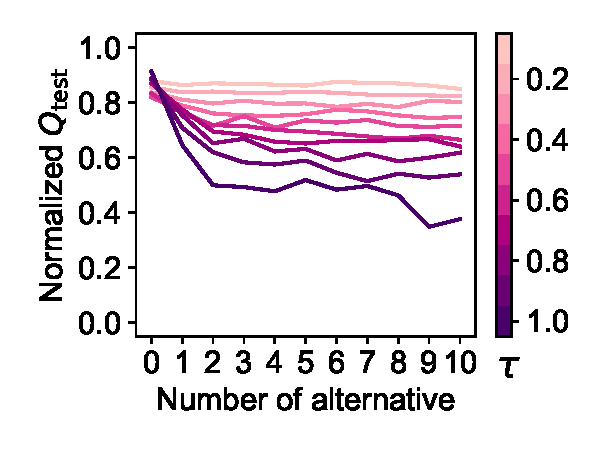
\includegraphics[width=\textwidth, trim=15 15 10 15, clip]{plots/afs-impact-num-alternatives-tau-test-objective-max.pdf}
		\caption{
			Test-set objective value, max-norma\-lized.
			Infeasible feature sets excluded.
		}
		\label{fig:afs:impact-num-alternatives-tau-test-objective-max}
	\end{subfigure}
	\hfill
	\begin{subfigure}[t]{0.48\textwidth}
		\centering
		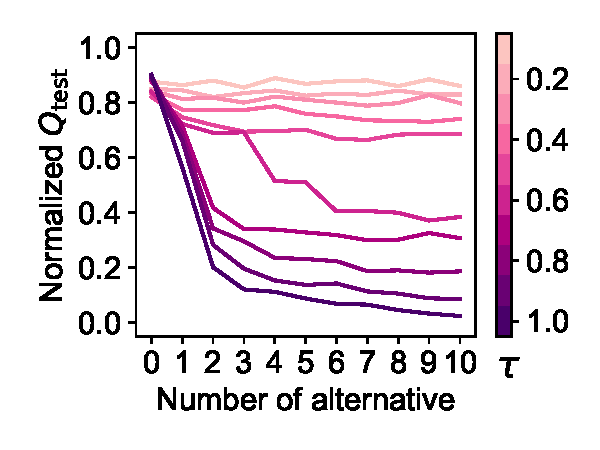
\includegraphics[width=\textwidth, trim=15 15 10 15, clip]{plots/afs-impact-num-alternatives-tau-test-objective-max-fillna.pdf}
		\caption{
			Test-set objective value, max-norma\-lized.
			Infeasible feature sets assigned a quality of~0.
		}
		\label{fig:afs:impact-num-alternatives-tau-test-objective-max-fillna}
	\end{subfigure}
	\\ \vspace{\baselineskip}
	\begin{subfigure}[t]{0.48\textwidth}
		\centering
		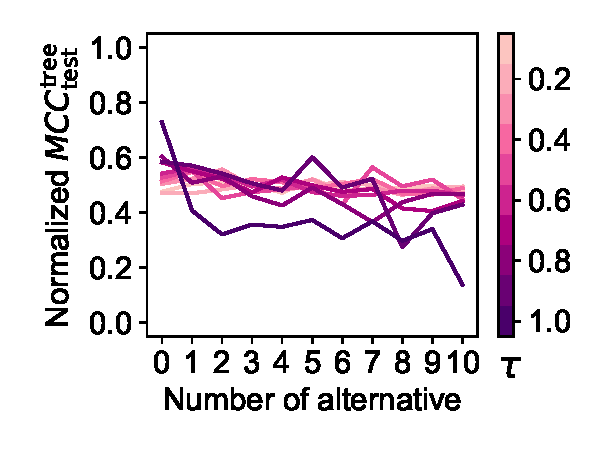
\includegraphics[width=\textwidth, trim=15 15 10 15, clip]{plots/afs-impact-num-alternatives-tau-decision-tree-test-mcc-min-max.pdf}
		\caption{
			Test set prediction performance, min-max-normalized.
			Infeasible feature sets excluded.
		}
		\label{fig:afs:impact-num-alternatives-tau-decision-tree-test-mcc-min-max}
	\end{subfigure}
	\hfill
	\begin{subfigure}[t]{0.48\textwidth}
		\centering
		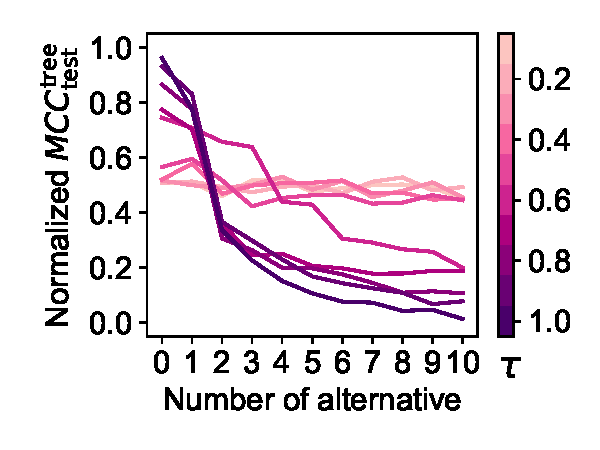
\includegraphics[width=\textwidth, trim=15 15 10 15, clip]{plots/afs-impact-num-alternatives-tau-decision-tree-test-mcc-min-max-fillna.pdf}
		\caption{
			Test set prediction performance, min-max-normalized.
			Infeasible feature sets assigned a quality of~0.
		}
		\label{fig:afs:impact-num-alternatives-tau-decision-tree-test-mcc-min-max-fillna}
	\end{subfigure}
	\caption{
		Mean of feature-set quality, normalized per experimental setting, over the number of alternatives and dissimilarity threshold~$\tau$, by evaluation metric.
		Results from sequential search with \emph{MI} as feature-selection method and $k=10$.
	}
	\label{fig:afs:impact-num-alternatives-tau-quality}
\end{figure}

\paragraph{Feature-set quality}

As Figure~\ref{fig:afs:impact-num-alternatives-tau-train-objective-max} shows for \emph{MI} as feature-selection method, the decrease of the objective value~$Q$ over the number of alternatives strongly depends on the dissimilarity threshold~$\tau$.
Note that we use results from $k=10$ instead of $k=5$ here to show more distinct values of $\tau$.
For a low dissimilarity threshold, e.g., $\tau=0.1$, the objective value barely drops over the number of alternatives.
In contrast, the objective value decreases significantly for a high dissimilarity threshold, e.g., $\tau=1$.
This is expected, since a higher~$\tau$ constrains the feature selection more by preventing the selection of previously selected features more strongly.
As Figure~\ref{fig:afs:impact-num-alternatives-tau-test-objective-max} displays, this phenomenon also holds for the test-set objective value, though the dependency on~$\tau$ is less prominent there.
In contrast, the effect of~$\tau$ on prediction performance exhibits a less clear trend, as visualized in Figure~\ref{fig:afs:impact-num-alternatives-tau-decision-tree-test-mcc-min-max}.
This result underlines our previous observation that the objective value is only partially indicate of prediction performance.

\begin{figure}[htbp]
	\centering
	\begin{subfigure}[t]{0.48\textwidth}
		\centering
		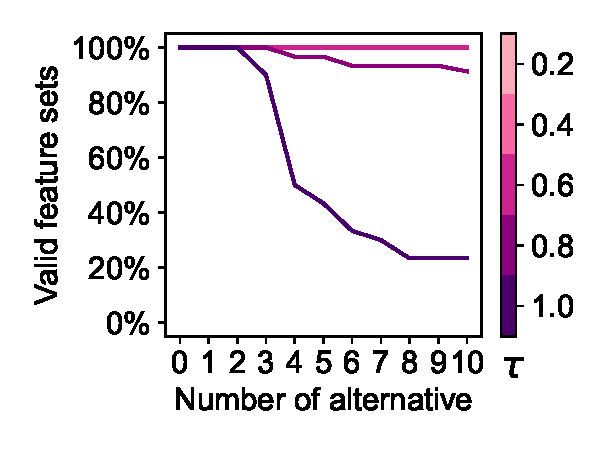
\includegraphics[width=\textwidth, trim=15 15 10 15, clip]{plots/afs-impact-num-alternatives-tau-optimization-status-k-5.pdf}
		\caption{Feature-set size~$k=5$.}
		\label{fig:afs:impact-num-alternatives-tau-optimization-status-k-5}
	\end{subfigure}
	\hfill
	\begin{subfigure}[t]{0.48\textwidth}
		\centering
		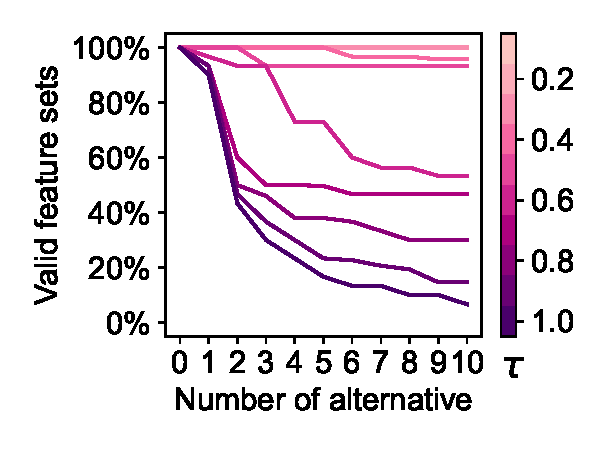
\includegraphics[width=\textwidth, trim=15 15 10 15, clip]{plots/afs-impact-num-alternatives-tau-optimization-status-k-10.pdf}
		\caption{Feature-set size~$k=10$.}
		\label{fig:afs:impact-num-alternatives-tau-optimization-status-k-10}
	\end{subfigure}
	\caption{
		Fraction of optimization runs yielding a valid feature set over the number of alternatives and dissimilarity threshold~$\tau$.
		Results from sequential search with \emph{MI} as feature-selection method.
	}
	\label{fig:afs:impact-num-alternatives-tau-optimization-status}
\end{figure}

\paragraph{Optimization status}

Similar to our previous analysis for the number of alternatives in Section~\ref{sec:afs:evaluation:search:num-alternatives}, one also needs to consider that setting~$\tau$ to certain values can make the optimization problem infeasible.
In particular, for a higher dissimilarity threshold, the likelihood is higher that there is no feature set that is alternative enough.
Figure~\ref{fig:afs:impact-num-alternatives-tau-optimization-status} visualizes how the fraction of valid feature sets develops over the number of alternatives and dissimilarity threshold~$\tau$.
Figures~\ref{fig:afs:impact-num-alternatives-tau-train-objective-max-fillna},~\ref{fig:afs:impact-num-alternatives-tau-test-objective-max-fillna}, and~\ref{fig:afs:impact-num-alternatives-tau-decision-tree-test-mcc-min-max-fillna} account for infeasible feature sets by setting their feature-set quality to zero.
Compared to Figures~\ref{fig:afs:impact-num-alternatives-tau-train-objective-max},~\ref{fig:afs:impact-num-alternatives-tau-test-objective-max}, and~\ref{fig:afs:impact-num-alternatives-tau-decision-tree-test-mcc-min-max}, the decrease in objective value is noticeably stronger.
In contrast, if only considering valid feature sets, the mean objective value can increase over the number of alternatives, as visible in Figure~\ref{fig:afs:impact-num-alternatives-tau-train-objective-max} for $\tau=1.0$ or in Figure~\ref{fig:afs:impact-num-alternatives-fs-method-train-objective-max} for \emph{MI} and \emph{Model Gain}.
This counterintuitive phenomenon can occur because some datasets run out of valid feature sets sooner than others, so the average quality is determined for different sets of datasets at each number of alternatives.

\begin{figure}[htb]
	\centering
	\begin{subfigure}[t]{0.48\textwidth}
		\centering
		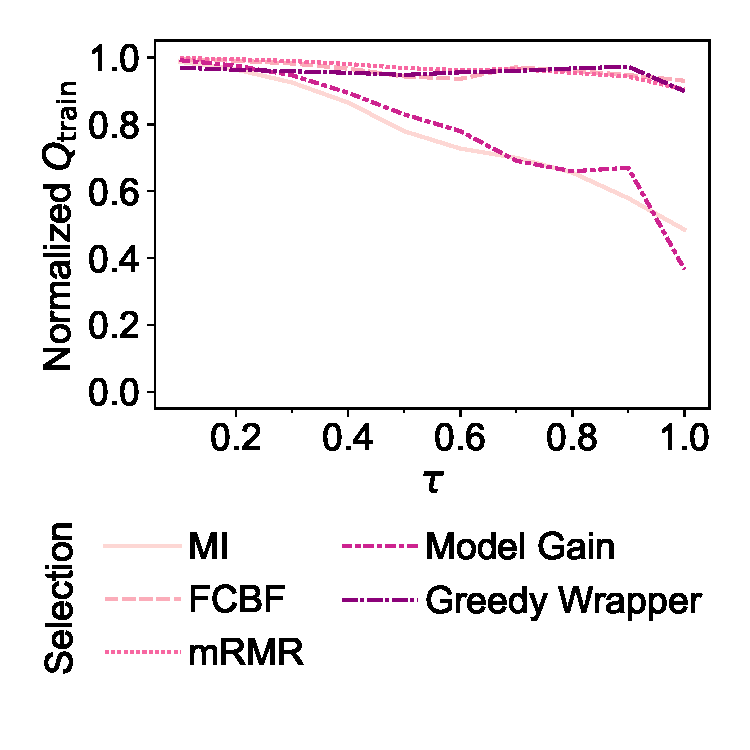
\includegraphics[width=\textwidth, trim=20 40 15 15, clip]{plots/afs-impact-tau-fs-method-train-objective-max.pdf}
		\caption{Training-set objective value.}
		\label{fig:afs:impact-tau-fs-method-train-objective-max}
	\end{subfigure}
	\hfill
	\begin{subfigure}[t]{0.48\textwidth}
		\centering
		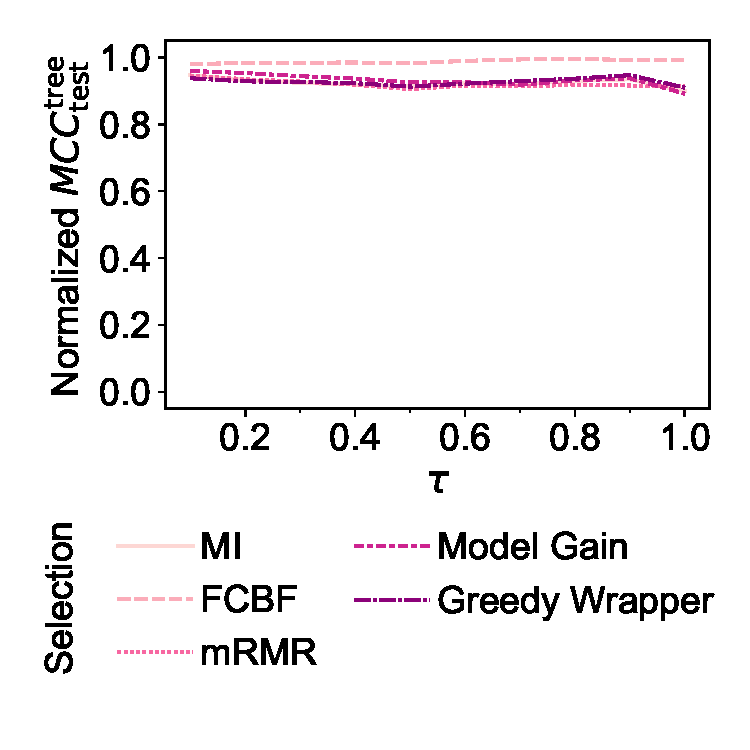
\includegraphics[width=\textwidth, trim=20 40 15 15, clip]{plots/afs-impact-tau-fs-method-decision-tree-test-mcc-max.pdf}
		\caption{Test-set prediction performance.}
		\label{fig:afs:impact-tau-fs-method-decision-tree-test-mcc-max}
	\end{subfigure}
	\caption{
		Median feature-set quality, max-normalized per experimental setting, over the dissimilarity threshold~$\tau$, by evaluation metric.
		Infeasible feature sets excluded.
		Results from sequential search with $k=10$.
	}
	\label{fig:afs:impact-tau-fs-method-quality}
\end{figure}

\paragraph{Influence of feature-selection method}

While the previous observations applied to \emph{MI} as feature-selection method, they do not hold universally, as Figure~\ref{fig:afs:impact-tau-fs-method-train-objective-max} shows.
Besides \emph{MI}, the objective value of \emph{Model Gain} strongly depends on~$\tau$ as well.
In contrast, the remaining three feature-selection methods exhibit less influence of~$\tau$ on the quality of found feature sets.
For \emph{Greedy Wrapper}, this outcome can be explained by the heuristic search procedure to find feature sets.
For \emph{FCBF}, the fraction of infeasible solutions is much higher than for \emph{MI} in general, so this aspect plays a larger role than the quality variation of found feature sets.
For \emph{mRMR}, the low influence of~$\tau$ matches the low influence of the number of alternatives.
For this feature-selection method, alternative feature sets seem to vary little in their objective value.

Despite different effects on the objective value, the effect of a higher~$\tau$ causing more infeasible feature sets remains for all feature-selection methods.
Further, the test-set prediction performance does not vary considerably over $\tau$ for any of the feature-selection methods, as Figure~\ref{fig:afs:impact-tau-fs-method-decision-tree-test-mcc-max} displays.

\subsection{Summary}
\label{sec:afs:evaluation:summary}

\paragraph{Datasets (cf.~Section~\ref{sec:afs:evaluation:datasets})}

Generally, feature-set quality strongly depended on the dataset.
Thus, an analysis of alternative feature sets needs be dataset-specific or appropriately normalize quality.

\paragraph{Feature-set quality metrics (cf.~Section~\ref{sec:afs:evaluation:metrics})}

Different notions of feature-set quality exhibited different patterns when we varied other experimental dimensions, so one should decide on a notion of feature-set quality carefully.
In particular, the objective function of simple feature-selection methods might disagree with actual prediction performance of the corresponding feature sets.
Further, we observed overfitting, i.e., a gap between training-set quality and test-set quality, also for simple objective functions, though to a lesser extent than for prediction performance.

\paragraph{Feature-selection methods (cf.~Section~\ref{sec:afs:evaluation:feature-selection})}

Among the feature-selection methods, \emph{Model Gain} resulted in the best prediction performance on average, though the simple univariate \emph{MI} also turned out competitive in that regard.
Further, \emph{Greedy Wrapper} and \emph{mRMR} required high optimization times, while our constrained-based version of \emph{FCBF} yielded many infeasible solutions.
Finally, selecting $k=10$ instead of $k=5$ features only yielded a small improvement for all feature-selection methods, so one might stick to smaller feature-set sizes if such a setting benefits interpretability for users.

\paragraph{Search methods for alternatives (cf.~Section~\ref{sec:afs:evaluation:search:method})}

Simultaneous search, particularly with the minimum-quality objective, considerably reduced the variance in the training-set objective value over alternatives compared to sequential search, as we desired.
However, results were less clear on the test set and when considering prediction performance to measure feature-set quality.
Further, the average quality of alternatives was similar between the search methods.
In addition, sequential search was considerably faster than the simultaneous one and thereby led to less solver timeouts, particularly when increasing the number of alternatives.
Also, sequential search allows users to stop search after each alternative instead of requiring the number of alternatives to be determined beforehand.
Thus, we recommend using sequential search.

\paragraph{Number of alternatives $a$ (cf.~Section~\ref{sec:afs:evaluation:search:num-alternatives})}

Feature-set quality showed the highest decrease from the original feature set to the first alternative but less beyond.
The strength of this decrease depended on the feature-selection method.
There usually were several alternatives of similar quality if such valid alternatives existed at all.
In particular, the frequency of infeasible solutions naturally increased with~$a$ due to the presence of more constraints.
Finally, the quality decrease was more prominent on the training set than on the test set.

\paragraph{Dissimilarity threshold $\tau$ (cf.~Section~\ref{sec:afs:evaluation:search:tau})}

As expectable, a higher dissimilarity threshold caused a stronger decrease of feature-set quality in terms of objective value for the feature-selection methods \emph{MI} and \emph{Model Gain}.
This result shows that usera can control a trade-off between quality and dissimilarity, making a use-case-specific decision.
However, results regarding prediction performance and for the other three feature-selection methods were less clear.
In any case, a higher~$\tau$ naturally caused more infeasible solutions, which users should be aware of.

\section{Conclusions and Future Work}
\label{sec:afs:conclusion}

In this section, we summarize our work (cf.~Section~\ref{sec:afs:conclusion:conclusion}) and give an outlook on potential future work (cf.~Section~\ref{sec:afs:conclusion:future-work}).

\subsection{Conclusions}
\label{sec:afs:conclusion:conclusion}

Obtaining interpretable solutions is a highly active research area in machine learning.
One way to foster interpretability is by selecting a small set of features for predictions.
Traditional feature-selection methods yield \emph{one} feature set with high quality, e.g., regarding prediction performance.
However, users might be interested in obtaining multiple, sufficiently different feature sets that, at the same time, have high quality.
Such alternative feature set might provide alternative explanations for predictions from the data.

In this article, we defined alternative feature selection as an optimization problem.
We formalized alternatives via constraints, which are independent from the feature-selection method, can be combined with other constraints on feature sets, and allow users to control alternatives according to their needs.
Additionally, Appendix~\ref{sec:afs:appendix:complexity} analyzes the complexity of this optimization problem.
Further, we presented approaches to solve the optimization problem for different categories of feature-selection methods.
Finally, we ran an evaluation with 30 classification datasets and five feature-selection methods.
We compared two search methods for alternatives and varied the number of alternatives as well as the threshold for being alternative.

\subsection{Future Work}
\label{sec:afs:conclusion:future-work}

There are several points for applying, extending, or modifying alternative feature selection.

\paragraph{Feature selection (objective function)}

One can search for alternatives with other feature-selection methods than the five we analyzed.
For wrapper feature selection, which requires black-box optimization, there are multiple ways to consider alternatives (cf.~Section~\ref{sec:afs:approach:objectives:black-box}).
As we saw in our experiments, achieving a high feature-set quality within a reasonable time frame poses a particular challenge for this category of feature-selection methods.
Further, our generic search procedures need adaptation to work for the category of embedded feature selection (cf.~Section~\ref{sec:afs:approach:objectives:embedding}), which we did not consider in our experiments.

\paragraph{Alternatives (constraints)}

One can vary the notion of alternatives (cf.~Sections~\ref{sec:afs:approach:problem} and~\ref{sec:afs:approach:constraints}), e.g., the set-dissimilarity measure, the definitions for multiple alternatives, or by using soft constraints instead of hard constraints.
While we tried to make general and straightforward decisions for each of these points, particular applications might demand other formal definitions of alternatives.

\paragraph{Simultaneous alternatives}

Our experiments (cf.~Section~\ref{sec:afs:evaluation:search:method}) as well as theoretical analysis (cf.~Section~\ref{sec:afs:approach:constraints:multiple}) revealed that simultaneous search scales badly with the number of alternatives.
One way to alleviate this is finding a more efficient problem formulation, e.g., by loosening the constraints for alternatives.
However, looser constraints bear the danger of allowing identical feature sets as valid alternatives.
Further, one can limit the solver runtime and take the intermediate results once the timeout is reached.
We already used a fixed timeout in our experiments, but studying the exact influence of different timeouts one the feature-set quality is a topic for future work.
Next, one can use a different solver, e.g., one that supports non-linear terms so the interaction variables and constraints from Equation~\ref{eq:afs:product-linear} become superfluous.
Finally, one can develop a heuristic rather than an exact search procedure.

\paragraph{Datasets}

Our evaluation builds on benchmark datasets from various domains.
While we could uncover several general trends, the existence and the quality of alternative feature sets clearly depends on the dataset (cf.~Section~\ref{sec:afs:evaluation:datasets}).
Thus, practitioners can use our generic approaches to search alternatives in domain-specific case studies.

\appendix

\section{Appendix}
\label{sec:afs:appendix}

In this section, we provide technical details and discuss approaches not used in our experiments.
First, we discuss aggregation functions to instantiate the simultaneous-search objective from Equation~\ref{eq:afs:afs-simultaneous} (cf.~Section~\ref{sec:afs:appendix:simultaneous-objective-aggregation}).
Second, we provide comprehensive definitions of the alternative-feature-selection problem, which we described over the course of Section~\ref{sec:afs:approach} (cf.~Section~\ref{sec:afs:appendix:complete-optimization-problem}).
Third, we discuss the computational complexity of said optimization problem (cf.~Section~\ref{sec:afs:appendix:complexity}).
Fourth, we present a greedy heuristic for univariate feature selection from Equation~\ref{eq:afs:univariate-filter} (cf.~Section~\ref{sec:afs:appendix:univariate-search-algorithm}).
Fifth, we discuss further objective functions for multivariate filter feature selection, which we introduced in Section~\ref{sec:afs:approach:objectives:white-box} (cf.~Section~\ref{sec:afs:appendix:multivariate-filter-objectives}).

\subsection{Aggregation Functions for Simultaneous Search}
\label{sec:afs:appendix:simultaneous-objective-aggregation}

Equation~\ref{eq:afs:afs-simultaneous} introduced the optimization problem of simultaneous search but did not define the aggregation function~$\text{agg}(\cdot)$ in the objective.
In this section, we discusses the two functions we use in our experiments, sum and minimum, as well as further approaches for handling the quality of multiple alternatives.

\paragraph{Summed-quality objective}

The arguably simplest way to aggregate the qualities of multiple feature sets is to sum them up.
This leads to the following \emph{summed-quality objective}:
%
\begin{equation}
	\max_{s^{(0)}, \dots, s^{(a)}} \sum_{i=0}^a Q(s^{(i)},X,y)
	\label{eq:afs:afs-simultaneous-sum-objective}
\end{equation}
%
While this objective fosters a high average quality of feature sets, it does not guarantee that the alternatives have similar quality, though the latter could be one of the reasons for searching simultaneously.
For example, consider univariate filter feature selection (cf.~Equation~\ref{eq:afs:univariate-filter}) with six features, the feature qualities~$q = (1,2,3,7,8,9)$, desired feature-set size~$k=3$, number of alternatives~$a=2$, and dissimilarity threshold~$\tau = 0.5$, which permits an overlap of at most one feature between feature sets here.
Sequential search yields the selection $s^{(0)} = (0,0,0,1,1,1)$, $s^{(1)} = (0,1,1,0,0,1)$, and $s^{(2)} = (1,0,1,0,1,0)$, with an optimal summed feature-set quality of $24+14+12=50$.
One simultaneous-search solution consists of the feature sets $s^{(0)} = (0,0,1,0,1,1)$, $s^{(1)} = (0,1,0,1,0,1)$, and $s^{(2)} = (1,0,0,1,1,0)$, with an optimal summed feature-set quality of $20+18+16=54$.
Another simultaneous-search solution is $s^{(0)} = (1,0,0,0,1,1)$, $s^{(1)} = (0,1,0,1,0,1)$, and $s^{(2)} = (0,0,1,1,1,0)$, with an optimal summed feature-set quality of $18+18+18=54$.
This example provides us with several insights.
First, sequential search yields worse quality than simultaneous search here, i.e., 50 vs.~54, due to its greedy search procedure.
Second, the three feature-set qualities of the sequential solutions, i.e., 24, 14, and~12, differ significantly.
Third, simultaneous search can yield multiple solutions that all share the same summed feature-set quality.
However, the feature-set qualities in the second solution, i.e., 18, 18, and~18, are more balanced than in the first solution, i.e., 20, 18, and~16.
With the summed-quality objective, both these solutions are optimal, which might not satisfy the user's needs in some scenarios.

\paragraph{Minimum-quality objective}

To actively foster balanced feature-set qualities in simultaneous search, we propose the following \emph{minimum-quality objective}:
%
\begin{equation}
	\max_{s^{(0)}, \dots, s^{(a)}} \min_{i \in \{0, \dots, a\}} Q(s^{(i)},X,y) \\
	\label{eq:afs:afs-simultaneous-min-objective}
\end{equation}
%
In the terms of social choice theory, this re-formulated objective uses an egalitarian rule instead of a utilitarian one~\cite{myerson1981utilitarianism}.
Note that optimizing either the summed-quality objective or the minimum-quality objective does not necessarily optimize the other one.
Previously, we already showed an example for a solution optimizing the summed-quality objective but not the minimum-quality objective.
In the following, we demonstrate the other direction.
For example, consider univariate filter feature selection (cf.~Equation~\ref{eq:afs:univariate-filter}) with six features, the feature qualities~$q = (1,4,5,6,10,11)$, desired feature-set size~$k=3$, number of alternatives~$a=1$, and dissimilarity threshold~$\tau = 0.5$, which permits an overlap of at most one feature between feature sets here.
One solution optimizing the minimum-quality objective is $s^{(0)} = (0,1,0,0,1,1)$ and $s^{(1)} = (0,0,1,1,0,1)$, with a summed feature-set quality of $25+22=47$.
Another solution is $s^{(0)} = (1,0,0,0,1,1)$ and $s^{(1)} = (0,0,1,1,0,1)$, with a summed feature-set quality of $22+22=44$.
While both solutions have the same minimum feature-set quality of~22, only the first solution optimizes the summed-quality objective.
In particular, the minimum-quality objective allows reducing the quality of feature sets that are above the current minimum of all feature sets.

From the technical perspective, Equation~\ref{eq:afs:afs-simultaneous-min-objective} has the disadvantage of being a non-linear expression regarding the decision variables $s^{(0)}, \dots, s^{(a)}$.
However, we can linearize it with the help of an auxiliary variable~$Q_{\text{min}}$ and one additional constraint per feature set:
%
\begin{equation}
	\begin{aligned}
		\max_{s^{(0)}, \dots, s^{(a)}} &\quad &Q_{\text{min}} & \\
		\text{subject to:} &\quad \forall i \in \{0, \dots, a\}: &Q_{\text{min}} &\leq Q(s^{(i)},X,y) \\
		&\quad & Q_{\text{min}} &\in \mathbb{R}
	\end{aligned}
	\label{eq:afs:afs-simultaneous-min-objective-linear}
\end{equation}
%
As we maximize~$Q_{\text{min}}$, this variable will implicitly assume the actual minimum value of~$Q(s^{(i)},X,y)$ with equality since the solution would not be optimal otherwise.
This situation relieves us from introducing further auxiliary variables that are usually necessary when linearizing maximum or minimum expressions~\cite{mosek2022modeling}.

\paragraph{Further approaches for balancing quality}

The minimum-quality objective provides no control or guarantee how much the feature-set qualities will actually differ between alternatives since it only incentives high quality for all feature sets.
One can alleviate this problem in several ways, particularly by adapting the objective and/or constraints.
First, theoretical problems related to alternative feature selection also use other objectives for balanced quality~\cite{korf2010objective, lawrinenko2017identical} (cf.~Section~\ref{sec:afs:appendix:complexity:uni-min-partitioning}).
E.g., one could minimize the difference in quality between the highest-quality feature set and the lowest-quality feature set.
Second, one could keep the summed-quality objective but explicitly constrain the minimum or maximum quality of all feature sets, or the difference between the feature sets' qualities.
However, such constraint-based approaches introduce one or several parameters bounding feature-set quality, which are difficult to determine a priori.
Third, one could consider balanced feature sets' qualities as another objective besides the maximizing the summed quality.
One can then optimize two objectives simultaneously, filtering results for Pareto-optimal solutions, or optimize a weighted combination of the two objectives.
In both cases, the user might need to define an acceptable trade-off between the two objectives.
It currently is an open question if always one solution exists that is jointly optimal for both objectives.
If yes, then optimizing a weighted combination of the two objectives would also optimize each of the two objectives on its own, assuming positive weights for each objective, e.g., equal weighting.

\subsection{Complete Specifications of the Optimization Problem}
\label{sec:afs:appendix:complete-optimization-problem}

In this section, we provide complete specifications of the alternative-feature-selection problem for sequential and simultaneous search.
In particular, we combine all relevant definitions and equations from Section~\ref{sec:afs:approach}.
For the objective, we consider an univariate filter feature-selection method, as defined in the Equation~\ref{eq:afs:univariate-filter}.
The corresponding feature qualities $q(\cdot)$ are constants in the optimization problem.
To measure feature-set dissimilarity for alternatives, we use the Dice dissimilarity from Equation~\ref{eq:afs:dice-rearranged-equal-size}.
The dissimilarity threshold~$\tau \in [0,1]$ is a user-defined constant.
Further, we assume that each feature set should have a fixed, user-defined size~$k \in \mathbb{N}$, as in our experiments.

\paragraph{Sequential alternatives}

In the sequential case, only one feature set~$F_s$ is variable.
In contrast, the existing feature sets $F_{\bar{s}} \in \mathbb{F}$ with their selection vectors $\bar{s}$ are constants in the optimization problem.
%
\begin{equation}
	\begin{aligned}
		\max_s &\quad & Q_{\text{uni}}(s,X,y) &= \sum_{j=1}^{n} q(X_{\cdot{}j},y) \cdot s_j \\
		\text{subject to:} &\quad \forall F_{\bar{s}} \in \mathbb{F}: & \sum_{j=1}^n s_j \cdot \bar{s}_j &\leq (1 - \tau) \cdot k \\
		&\quad & \sum_{j=1}^n s_j &= k \\
		&\quad & s &\in \{0,1\}^n
	\end{aligned}
	\label{eq:afs:afs-sequential-complete}
\end{equation}
%
\paragraph{Simultaneous alternatives}

In the simultaneous case, all feature sets are variable.
Let~$a \in \mathbb{N}$ denote the number of alternatives, which corresponds to the number of feature sets minus one.
Further, we introduce auxiliary variables according to Equation~\ref{eq:afs:product-linear} to linearize products between variables.
Also, we use the summed-quality objective from Equation~\ref{eq:afs:afs-simultaneous-sum-objective}.
%
\begin{equation}
	\begin{aligned}
		\max_{s^{(0)}, \dots, s^{(a)}} &\quad & \sum_i Q_{\text{uni}}(s^{(i)},X,y) &= \sum_i \sum_j q(X_{\cdot{}j},y) \cdot s^{(i)}_j\\
		\text{subject to:} &\quad \forall i_1~\forall i_2: & \sum_j t^{(i_1,i_2)}_j &\leq (1 - \tau) \cdot k \\
		&\quad \forall i_1~\forall i_2~\forall j: & t^{(i_1,i_2)}_j &\leq s^{(i_1)}_j \\
		&\quad \forall i_1~\forall i_2~\forall j: & t^{(i_1,i_2)}_j &\leq s^{(i_2)}_j \\
		&\quad \forall i_1~\forall i_2~\forall j: & 1 + t^{(i_1,i_2)}_j &\geq s^{(i_1)}_j + s^{(i_2)}_j \\
		&\quad \forall i: & \sum_j s^{(i)}_j &= k \\
		&\quad \forall i: & s^{(i)} &\in \{0,1\}^n \\
		&\quad \forall i_1~\forall i_2: & t^{(i_1,i_2)} &\in \{0,1\}^n \\
		\text{with indices:} &\quad & i &\in \{0, \dots, a\} \\
		&\quad & i_1 &\in \{1, \dots, a\} \\
		&\quad & i_2 &\in \{0, \dots, i_1-1\} \\
		&\quad & j &\in \{1, \dots, n\}
	\end{aligned}
	\label{eq:afs:afs-simultaneous-complete}
\end{equation}

\subsection{Complexity of the Optimization Problem}
\label{sec:afs:appendix:complexity}

In this section, we discuss the time complexity of alternative feature selection as defined in Section~\ref{sec:afs:approach}.
In particular, we are interested in scalability regarding the number of features~$n \in \mathbb{N}$, also considering the feature-set size~$k \in \mathbb{N}$ and the number of alternatives~$a \in \mathbb{N}_0$.
Section~\ref{sec:afs:appendix:complexity:exhaustive} discusses exhaustive search, which works for arbitrary feature-selection methods.
The four subsequent sections analyze univariate filter feature selection in detail:
Section~\ref{sec:afs:appendix:complexity:uni} provides a general analysis, while Sections~\ref{sec:afs:appendix:complexity:uni-min-partitioning} and~\ref{sec:afs:appendix:complexity:uni:min-no-partitioning} investigate the minimum-quality objective in particular and Section~\ref{sec:afs:appendix:complexity:uni-sum} examines the summed-quality objective.
Finally, Section~\ref{sec:afs:appendix:complexity:summary} summarizes our key results and Section~\ref{sec:afs:appendix:complexity:future} outlines potential future work.

\subsubsection{Exhaustive Search for Arbitrary Feature-Selection Methods}
\label{sec:afs:appendix:complexity:exhaustive}

The arguably simplest solution approach for alternative feature selection is an exhaustive search over the entire search space.
For each solution candidate, such an approach needs to check the validity of the constraints for alternatives.
Further, for valid solution candidates, it needs to evaluate the objective function, i.e., determine feature-set quality.

We analyze exhaustive search since it provides an upper bound for the time complexity of a runtime-optimal search algorithm.
In this section, we assume unit costs for elementary arithmetic operations like addition, multiplication, and comparison of two numbers.

\paragraph{Traditional feature selection}

In general, the search space of feature selection grows exponentially with~$n$, even without considering alternatives.
In particular, there are $2^n - 1$ possibilities to form a single non-empty feature set of arbitrary size.
For a feature set of fixed size~$k$, as in our experiments, there are $\binom{n}{k} = \frac{n!}{k! \cdot (n-k)!}$ solution candidates.
In an exhaustive search, we can directly enumerate these feature sets and thereby ignore the ones violating the cardinality constraint.

The asymptotic growth of the binomial expression regarding~$n$ depends on~$k$.
Generally, the number of possible feature sets is in~$O(n^k)$ since $\binom{n}{k} \leq n^k$.
If we consider~$k$ to be a small constant and independent from~$n$, i.e., $k \ll n,~k \in O(1)$, then the complexity is polynomial in~$n$.
This assumption makes sense in feature selection, where one typically wants to obtain a low-dimensional subset of a high-dimensional dataset.
However, the exponent~$k$ might still render an exhaustive search practically infeasible.
In terms of parametrized complexity, the problem resides in class~$\mathcal{XP}$ since the runtime term has the form $O(f(k) \cdot n^{g(k)})$~\cite{downey1997parameterized}, here with parameter~$k$ and functions $f(k) = 1$, $g(k) = k$.

Note that we have ignored the effort for computing the quality of each feature set within the search yet.
This effort depends on the feature-selection method but should usually be polynomial in~$n$ as well.
Even better, since feature-set quality typically only depends on selected features rather than unselected ones, the effort might be polynomial in~$k \ll n$.

\paragraph{Sequential search}

Like traditional feature selection, sequential search (cf.~Definition~\ref{def:afs:sequential-alternative}) targets at finding a single feature set at once.
Thus, the search space is the same.
Unlike traditional feature selection, not all size-$k$ feature sets are valid anymore.
In particular, the constraints for being alternative put an extra effort on each solution candidate in the search.
As Equation~\ref{eq:afs:afs-sequential-complete} shows, checking constraints involves iterating over all existing feature sets and features to compute the dissimilarity between feature sets.
This procedure entails an effort of~$O(a \cdot n)$ for one alternative.
For the whole sequential procedure, yielding a total of~$a$ alternatives, the effort becomes~$O(a^2 \cdot n)$.
Combining this effort with exhaustive search over size-$k$ feature sets, we obtain the following proposition:
%
\begin{proposition}[Complexity of exhaustive sequential search]
	Exhaustive sequential search for $a \in \mathbb{N}$ alternative feature sets of size~$k$ from $n$~features has a time complexity of~$O(a^2 \cdot n^{k+1})$ without the effort for evaluating the objective function.
	\label{prop:afs:complexity-exhaustive-sequential}
\end{proposition}
%
Thus, the runtime remains polynomial under the assumption $k \ll n,~k \in O(1)$ and generally belongs to the parameterized complexity class~$\mathcal{XP}$ with~$k$ as parameter.
In case we only store feature sets of size~$k$ instead of the complete selection vectors of size~$n$, we can reduce effort for constraint checking and obtain an overall time complexity of~$O(a^2 \cdot k \cdot n^k)$.

\paragraph{Simultaneous search}

Simultaneous search (cf.~Definition~\ref{def:afs:simultaneous-alternative}) enlarges the search space since it optimizes $a+1$ feature sets at once.
Thus, an exhaustive search over size-$k$ feature sets iterates over~$O(n^{k \cdot (a+1)})$ solution candidates.
As for sequential search, there is a small additional effort for constraint checking.
Thus, we arrive at the following proposition:
%
\begin{proposition}[Complexity of exhaustive simultaneous search]
	Exhaustive simultaneous search for $a + 1$~alternative feature sets of size~$k$ from $n$~features has a time complexity of~$O(a^2 \cdot n^{k \cdot (a+1) + 1})$ without the effort for evaluating the objective function.
	\label{prop:afs:complexity-exhaustive-simultaneuos}
\end{proposition}
%
The scalability with~$n$ is clearly worse than for sequential search since the number of alternatives also appears in the exponent now.
For parameterized complexity, the problem is again in class $\mathcal{XP}$ with the parameter~$a \cdot k$.
Assuming~$a$ and~$k$ to be small and independent from~$n$, the time complexity is still polynomial in~$n$ but with a even worse exponent than in sequential search.

Additionally, Proposition~\ref{prop:afs:complexity-exhaustive-simultaneuos} assumes that constraint checking does not require linearization variables like $t^{(i_1,i_2)}_j$ in Equation~\ref{eq:afs:afs-simultaneous-complete}, which would increase the search space even further.
Further, note that choosing between the summed-quality objective (cf.~Equation~\ref{eq:afs:afs-simultaneous-sum-objective} and the minimum-quality objective (cf.~Equation~\ref{eq:afs:afs-simultaneous-min-objective}) does not affect the complexity in exhaustive search, since computing both objectives requires one pass over all feature-set qualities.

Finally, the complexity is lower for the special case~$0 < \tau \cdot k \leq 1$, i.e., if feature sets need to differ in only one feature.
This implies that each feature set is alternative to each other feature set unless both sets are identical.
Thus, each set of $a + 1$ feature sets constitutes a valid solution, with no further constraint checking necessary.
Hence, instead of iterating over sets of feature sets, once can iterate over individual feature sets and maintain a buffer with the $a + 1$ feature sets with highest quality.
For each feature set iterated over, one needs to determine if its quality is higher than the lowest feature-set quality in the buffer:
If yes, replace the corresponding feature set in the buffer, if no, leave the buffer unchanged.
After iterating, this buffer contains the jointly optimal solution for the minimum-quality objective and the summed-quality objective.
This procedure has a runtime of $O((a + 1) \cdot n^k)$ without the effort for evaluating the objective function.
I.e., unlike in Proposition~\ref{prop:afs:complexity-exhaustive-simultaneuos}, $a$ is not part of the exponent anymore and the effort corresponds to the search for one feature set times the desired number of alternatives.
For large $a$, one can implement the buffer as a heap and thereby even reduce the linear factor regarding~$a$ to a logarithmic one.

\subsubsection{Univariate Filter Feature Selection}
\label{sec:afs:appendix:complexity:uni}

\paragraph{Motivation}

While assumptions like $a \cdot k \in O(1)$ ensure polynomial runtime for alternative feature selection with arbitrary objectives, the optimization problem without these assumptions can still be hard.
In the following, we derive complexity results for univariate filter feature selection (cf.~Equation~\ref{eq:afs:univariate-filter} and Section~\ref{sec:afs:appendix:complete-optimization-problem}).
This feature-selection method has the arguably simplest objective function, i.e., a feature set's quality equals the sum of its constituent features' qualities.
This simplicity does not only make the objective's evaluation cheap but also eases a transformation from and to well-known $\mathcal{NP}$-hard problems with comparably straightforward objectives.

\paragraph{Relationship to integer-programming problem}

As used in our implementation and analyzed in Section~\ref{sec:afs:approach:objectives:white-box}, the univariate objective and several other feature-selection methods allow to formulate alternative feature selection as a 0-1 integer linear program.
In particular, the constraints for being alternative are integer linear expressions or can be linearized.
The same goes for the minimum-quality and the summed-quality objective (cf.~Section~\ref{sec:afs:appendix:simultaneous-objective-aggregation}).
\textsc{Integer programming} is an $\mathcal{NP}$-complete problem in general, even for binary decision variables like we have~\cite{garey2003computers, karp1972reducibility}.
Thus, alternative feature selection with a white-box objective suitable for \textsc{Integer programming} cannot be harder than $\mathcal{NP}$.
However, since alternative feature selection only uses special types of constraints instead of expressing arbitrary integer linear problems, it could still be easier.
Vice versa, the membership in $\mathcal{NP}$ based on \textsc{Integer programming} assumes a particular encoding of alternative feature selection, i.e., storing each constraint separately.
If we instead define the problem's input size only as the number of features~$n$ or the total encoding length of the objective function plus parameters~$a$, $k$, and $\tau$, the problem could theoretically be harder than $\mathcal{NP}$, e.g., for a higher number of alternatives.
In particular, increasing the number of alternatives would only increase the encoding length logarithmically but the effort for constraint checking quadratically.

\paragraph{Leveraging monotonicity}

The univariate filter criterion is monotonic in the individual features' qualities and the feature-selection decision.
In particular, selecting more features cannot decrease the objective.
Further, given a fixed feature-set size, replacing one feature with another feature of higher quality cannot decrease the objective.
When aggregating over feature sets in simultaneous search, the summed-quality objective and the minimum-quality-objective (cf.~Equations~\ref{eq:afs:afs-simultaneous-sum-objective} and~\ref{eq:afs:afs-simultaneous-min-objective}) are monotonic as well.

These observations allow speeding up alternative feature selection with univariate qualities.
In particular, assuming $(a + 1) \cdot k < n$, it is sufficient to use the $(a + 1) \cdot k$ highest feature qualities when searching for an optimal solution out of $a + 1$ feature sets.
Due to monotonicity, the remaining feature qualities cannot improve the objective.
Thus, one can drop the remaining feature qualities in a pre-selection step before the actual search.
Note that there might be further optimal solutions, i.e., with same objective value, using the dropped features.
For example, such solutions can arise in case of multiple identical qualities or for the minimum-quality objective.
Still, if one only wants to find one optimal solution, working with the top $(a + 1) \cdot k$ features is sufficient.
The solution itself might not use all of these top features, i.e., the proposed pre-selection is an over-approximation in that regard.

Assuming sufficiently small, constant $a$ and $k$ again, i.e., $a \cdot k \in O(1)$, the pre-selection causes the number of relevant feature-set qualities and thereby the pure search effort to become independent from~$n$, which is even better than the polynomial runtime for general objectives under that assumption (cf.~Section~\ref{sec:afs:appendix:complexity:exhaustive}).
However, one needs to determine the highest feature qualities first.
To that end, one can either sort all qualities in~$O(n \cdot \log n)$ or iteratively determine the maximum quality in~$O((a+1) \cdot k \cdot n)$, which is $O(n)$ for small, constant~$a$ and~$k$.

\subsubsection{Univariate Minimum-Quality Objective with Complete Partitioning}
\label{sec:afs:appendix:complexity:uni-min-partitioning}

\paragraph{Assumptions}

A special case of alternative feature selection results from permitting zero overlap of feature sets, i.e., a dissimilarity threshold of~$\tau = 1$.
Thus, simultaneous search, which we analyze in the following, partitions the features into $a+1$ `actual' feature sets and potentially a $a+2$-th `dummy' set containing all remaining features.
If the latter exists, we speak of a \emph{incomplete partitioning}, else a \emph{complete partitioning}.
In case all feature sets have size~$k$, a complete partitioning implies that~$n = (a+1) \cdot k$.
Note that this scenario explicitly violates the prior assumptions we made for polynomial-runtime claims.

A key factor driving the hardness of partitioning problems is the shear number of solution candidates.
In particular, the number of ways to partition a set of $n$~elements into $a$~non-empty subsets equals $\stirling{n}{a}$, a Stirling number of the second kind~\cite{graham1994concrete}.
These numbers roughly scale like $a^n / a!$~\cite{moser1958stirling}, which is exponential in~$n$ given a fixed~$a$.
Even if the subset sizes are fixed, the number of valid partitioning solutions retains its awful scalability regarding~$n$ since it bases on a multinomial coefficient.

\paragraph{Related $\mathcal{NP}$-complete problems}

There are several $\mathcal{NP}$-complete problems that involve partitioning a set of elements into non-overlapping subsets~\cite{garey2003computers}.
E.g., \textsc{Partition}~\cite{karp1972reducibility} asks if one can partition a set of elements with positive integer weights into two subsets with the same sum over their elements weights.
\textsc{3-Partition}~\cite{garey2003computers} demands a partitioning into subsets containing three elements whose positive integer weights all sum up to one particular pre-defined number.
In contrast to these two problems, we do not require alternative feature sets to have exactly the same quality.
\textsc{Multi-Way Number Partitioning} requires partitioning a multiset of $n$~integers into $a$~subsets such that the sums of all subsets are as equal as possible~\cite{korf2010objective}.
We focus on this problem in the following.

\paragraph{Unconstrained feature-set size}

Different objectives formalize notion of desiring balanced subset sums; these objectives can lead to different optimal solutions~\cite{korf2010objective, lawrinenko2017identical}.
The most prominent problem formulation, denoted as \textsc{Multiprocessor Scheduling} in~\cite{garey2003computers}, minimizes the maximum sum of all subsets~\cite{lawrinenko2018reduction, walter2017improved}.
Figuratively speaking, the goal is to assign given tasks with positive integer lengths to a fixed number of processors such that the maximum over the summed runtime of all processors is minimal.
Multiplying all task lengths with~$-1$, one can turn the minimax problem of \textsc{Multiprocessor Scheduling} into the maximin formulation of simultaneous search with the minimum-quality objective.
Thereby, the tasks of \textsc{Multiprocessor Scheduling} correspond to features, the negated versions of the task lengths become univariate feature qualities, and the processors turn into feature sets. 
Since \textsc{Multiprocessor Scheduling} is $\mathcal{NP}$-complete, even for just two partitions~\cite{garey2003computers}, and our transformed problem requires the same effort for checking the validity of solutions, our problem is $\mathcal{NP}$-complete as well:
%
\begin{proposition}[Complexity of simultaneous search with minimum-quality objective, $\tau=1$, complete partitioning, and unconstrained feature-set size]
	Assuming univariate feature qualities, a dissimilarity threshold~$\tau = 1$, unconstrained feature-set sizes, and all $n$~features have to be selected, simultaneous search for $a+1$ alternative feature sets with the minimum-quality objective is $\mathcal{NP}$-complete.
	\label{prop:afs:complexity-partitioning-min-unconstrained-k}
\end{proposition}
%
Since the assumptions in Proposition~\ref{prop:afs:complexity-partitioning-min-unconstrained-k} denote a special case of alternative feature selection, we directly obtain the following, more general corollary:
%
\begin{corollary}[Complexity of simultaneous search with minimum-quality objective]
	Simultaneous search for alternative feature sets with the minimum-quality objective is $\mathcal{NP}$-hard.
	\label{corr:afs:complexity-sim}
\end{corollary}
%
There are several exact algorithms for \textsc{Multi-Way Number Partitioning}, e.g., using branch-and-bound approaches, that might have exponential runtime~\cite{haouari2008maximizing, schreiber2018optimal, walter2017improved}.
However, for a fixed number of partitions, the problem is only $\mathcal{NP}$-complete in the weak sense since it admits pseudo-polynomial algorithms~\cite{garey2003computers, korf2009multi}.
Such algorithms run in polynomial time if the input numbers are bounded to a certain size known in advance.
Since our feature qualities typically are real numbers in $[0,1]$, one would need to scale and discretize them to make such an algorithm feasible.
Also, for an arbitrary number of partitions, the problem is $\mathcal{NP}$-complete in the strong sense, which means that no pseudo-polynomial algorithm can exist unless $\mathcal{P}=\mathcal{NP}$~\cite{garey2003computers}.

However, $\mathcal{NP}$-completeness does not exclude the existence of approximation routines that run in polynomial time and have a guaranteed quality relative to the optimal solution.
For example, \cite{alon1998approximation, deuermeyer1982scheduling, woeginger1997polynomial}~present such polynomial-time algorithms for the maximin formulation of \textsc{Multi-Way Number Partitioning}, which corresponds to our minimum-quality objective.
In particular, \cite{alon1998approximation, woeginger1997polynomial} describe polynomial-time approximation schemes (PTAS), which can provide a solution arbitrarily close to the optimum.
However, the runtime depends on the desired approximation ratio and can grow exponential the more precision is desired.
In particular, unless $\mathcal{P}=\mathcal{NP}$, the strong $\mathcal{NP}$-completeness of the problem prevents the existence of a fully polynomial-time approximation scheme (FPTAS), which would only polynomially depend on the precision of approximation~\cite{alon1998approximation, woeginger1997polynomial}.
However, a FPTAS does exist for each fixed number of partitions~\cite{sahni1976algorithms}.
Further, besides approximation algorithms, the problem also has polynomial-time exact algorithms assuming certain parameters of the problem to be fixed, e.g., the number of distinct numbers to be partitioned, i.e., feature qualities, or the largest number, i.e., feature quality~\cite{mnich2018parameterized}.
Thus, the problem is fixed-parameter tractable ($\mathcal{FPT}$) for an appropriate definition of `parameter'.

\paragraph{Constrained feature-set size}

Note that the previous discussion considered feature sets of arbitrary sizes.
However, feature selection in general, and our article in particular, typically work with a fixed feature-set size~$k$.
There are corresponding number-partitioning problems for this setting as well, e.g., called \textsc{Balanced Number Partitioning} or \textsc{K-Partitioning}.
The problems formulations differ in their objective and cardinality constraints.
E.g., \cite{babel1998thek, michiels2012computer, zhang2011heuristic} require partitions of identical size but employ a minimax rather than a maximin objective.
However, as for the unconstrained case, we can multiply all numbers with -1 and thereby obtain a problem instance with our minimum-quality objective.
Based on the $\mathcal{NP}$-hardness of \textsc{K-Partitioning}~\cite{babel1998thek} and the polynomial time required to check a solution, we obtain the following proposition:
%
\begin{proposition}[Complexity of simultaneous search with minimum-quality objective, $\tau=1$, complete partitioning, and constrained feature-set size]
	Assuming univariate feature qualities, a dissimilarity threshold~$\tau = 1$, desired feature-set size~$k$, and all $n$~features have to be selected, simultaneous search for $n/k$ alternative feature sets with the minimum-quality objective is $\mathcal{NP}$-complete.
	\label{prop:afs:complexity-partitioning-min-constrained-k}
\end{proposition}
%
For the minimax objective, \cite{babel1998thek, michiels2012computer, zhang2011heuristic} propose heuristic algorithms, some of them with guaranteed approximation ratios.
\cite{babel1998thek} also provides a bound of the optimal objective value with cardinality constraints relative to the unconstrained case.
Further, there is a polynomial-time approximation scheme (PTAS) for each fixed partition size~$k$~\cite{michiels2012computer}.
Finally, the problem exhibits a polynomial-time exact algorithm for the special case $k=2$~\cite{dellamico2004heuristic, dellamico2001bounds} and a fully polynomial-time approximation scheme (FPTAS) for $k=n/2$~\cite{woeginger2005comment}.

One can also loosen the cardinality constraints by using upper bounds instead of strict equalities, i.e., requiring $\leq k$ instead of $= k$.
Further, the prescribed cardinality might vary between partitions instead of being the same~$k$ for all of them.
This generalized problem is $\mathcal{NP}$-hard in the strong sense but has heuristics running in polynomial time~\cite{kellerer2011a32approximation}.
In particular, \cite{chen2016efficient} provides an efficient polynomial-time approximation scheme (EPTAS).

As another problem formulation, \cite{chen20023partitioning, he2003kappa, lawrinenko2018reduction} use a maximin objective like we do.
This objective in combination with cardinality constraints was rarely addressed in literature~\cite{lawrinenko2018reduction}.
Note that all the three mentioned references use $\leq k$ constraints instead of $= k$ as in our experiments.
Again, this problem is $\mathcal{NP}$-hard in the strong sense~\cite{he2003kappa, lawrinenko2018reduction}, but \cite{chen20023partitioning, he2003kappa, lawrinenko2018reduction} propose approximation algorithms, partly with quality guarantees.

\subsubsection{Univariate Minimum-Quality Objective without Complete Partitioning}
\label{sec:afs:appendix:complexity:uni:min-no-partitioning}

Propositions~\ref{prop:afs:complexity-partitioning-min-unconstrained-k} and~\ref{prop:afs:complexity-partitioning-min-constrained-k} established $\mathcal{NP}$-completeness for problem instances requiring a complete partitioning of features.
The latter entails two assumptions, i.e., zero overlap between feature sets and each feature being selected exactly once.
Thereby, the choice of the user-defined parameters for alternative selection, i.e.,~$a$, $k$, and~$\tau$, is severely limited and might not reflect many real-world scenarios.
In this section, we show $\mathcal{NP}$-hardness for problem instances where these two assumptions do not hold.
We maintain the assumptions of using univariate feature qualities and the minimum-quality objective.

\paragraph{Incomplete partitioning}

A complete-partitioning scenario ties two parameters of alternative feature selection, i.e., the feature-set size~$k$ and number of alternatives~$a$, to the total number of features~$n$ by the equation~$n = (a+1) \cdot k$.
However, in practice, one might set these parameters such that some features are not part of any feature set.
In the following, we show that the problem of finding such an incomplete partitioning still is $\mathcal{NP}$-complete in general.

Let us assume to have an arbitrary problem instance~$I$ of the complete-partitioning problem.
Further, let the feature-set size~$k$ be fixed.
If we add one further feature~$f'$ to this problem instance and keep $a$, $k$, and $\tau$ as before, we obtain an instance~$I'$ of the incomplete-partitioning problem since one feature will not be selected.
We choose the quality~$q'$ of~$f'$ to be lower than the quality of all existing features in~$I$.
Given the monotonicity of the minimum-quality objective, adding feature~$f'$ to a feature set in the solution of~$I'$ does not have any benefit since~$f'$ would replace a feature with higher quality.
If~$f'$ is not selected, then this solution of~$I'$ also solves~$I$.
However, if the qualities of the resulting alternative feature sets are not equal, $f'$ might still be chosen for a feature set that does not have the minimum quality of all feature sets, since only the latter determines the overall objective value.
In that case, we can simply replace $f'$ with the feature that was not selected instead; the objective value remains the same and the solution becomes valid for~$I$.
Thus, in any case, we can easily transform a solution for~$I'$ to a solution for~$I$.

The previous argument shows that an algorithm for incomplete-partitioning problem instances can also solve arbitrary complete-partitioning problem instances with negligible computational overheard.
Thus, if a polynomial-time algorithm for incomplete partitioning existed, it could also solve complete partitioning in polynomial time.
However, we know the latter problem type to be $\mathcal{NP}$-complete (cf.~Proposition~\ref{prop:afs:complexity-partitioning-min-constrained-k}).
As a consequence, incomplete partitioning has to be $\mathcal{NP}$-hard.
Since checking a solution for an incomplete-partitioning problem instance is possible in polynomial time, we obtain membership in $\mathcal{NP}$ and thereby $\mathcal{NP}$-completeness.

To sum this up, we formulate the following proposition:
%
\begin{proposition}[Complexity of simultaneous search with minimum-quality objective, $\tau=1$, incomplete partitioning, and constrained feature-set size]
	Assuming univariate feature qualities, a dissimilarity threshold~$\tau = 1$, desired feature-set size~$k$, and \emph{not} all $n$~features have to be selected, simultaneous search for $a + 1$~alternative feature sets with the minimum-quality objective is $\mathcal{NP}$-complete.
	\label{prop:afs:complexity-incomplete-partitioning-min-constrained-k}
\end{proposition}

\paragraph{Overlapping feature sets}

Partitioning scenarios prevent overlap of feature sets by fixing the parameter~$\tau = 1$.
In the following, we show that allowing $0 < \tau < 1$ also results in an $\mathcal{NP}$-hard problem in general.
We do not consider $\tau = 0$ since such problem instances have the same time complexity as the underlying feature-selection problem without alternatives.

Again, let us assume to have an arbitrary problem instance~$I$ of the complete-partitioning problem.
Further, let the feature-set size~$k$ be fixed.
As before, we define a new problem instance~$I'$ by adding a new feature~$f'$.
However, this time, we increase the desired feature-set size to $k' = k + 1$.
Further, we set $\tau' = (k' - 1) / k'$, thereby allowing an overlap of at most one feature between feature sets.
Also, we choose~$f'$ to have a considerably higher feature-set quality than all other features.
The goal is to force the selection of~$f'$ in all feature sets since any selection not involving it would be worse, no matter which other features are selected.
One possible choice is setting $q' = \sum_{j=1}^n q_j + \varepsilon$, with $\varepsilon \in \mathbb{R}_{\geq 0}$ being a small positive number, or, if the qualities are integers, $\varepsilon = 1$.
Hence, the quality of~$f'$ is higher than the quality of selecting all original features from~$I$.
If we now obtain a solution for~$I'$, it contains~$f'$ in each feature set while the remaining features are part of exactly one feature set.
Thus, we can remove~$f'$ to get feature sets of size~$k = k' - 1$ that constitute an optimal solution for the original problem instance~$I$.

This transformation shows how problem instances with $\tau < 1$ can help solve arbitrary problem instances with $\tau = 1$.
Given the $\mathcal{NP}$-completeness of the latter problem, we obtain $\mathcal{NP}$-hardness of the former:
%
\begin{proposition}[Complexity of simultaneous search with minimum-quality objective, $\tau < 1$, and constrained feature-set size]
	Assuming univariate feature qualities, a dissimilarity threshold~$\tau < 1$, and desired feature-set size~$k$, simultaneous search for $a + 1$~alternative feature sets with the minimum-quality objective is $\mathcal{NP}$-hard.
	\label{prop:afs:complexity-no-partitioning-min-constrained-k}
\end{proposition}
%
Note that adding the proposed~$f'$ with a high quality~$q'$ enlarges the size of the problem instance to some extent.
However, the proposed transformation from $I$ to $I'$ is still possible in polynomial time and increases the input size by at most a fixed factor.
In particular, the encoding of a problem instance involves $n$~feature qualities as well as the values of $a$, $k$, and $\tau$.
Let us assume the feature qualities in $I$ have an average encoding size of $c \in \mathbb{R}$, so the overall encoding of the feature qualities has the size $c \cdot n$.
As the new feature~$f'$ corresponds to the sum of all feature qualities plus a small~$\epsilon$, its encoding size is upper-bounded by $c \cdot n$ if we disregard~$\epsilon$.
The change of $k$ and $\tau$ is negligible for the encoding size.
In consequence, the input size of~$I'$ is at most roughly double the size of~$I$.
If we explicitly stored all the constraints for alternatives and cardinality instead of only the relevant parameters, we would obtain a similar result.
In particular, all constraints would need to accommodate one new feature, independent of its feature quality.
Thus, the encoding size of each constraint would increase from $O(n)$ to $O(n+1)$, i.e., less than double.

The reduction above does not only work for $\tau' = (k' - 1) / k'$ but can be extended to all other $\tau > 0$.
In particular, for a fixed feature set-size~$k$, there is only a finite number of $\tau$ values leading to different overlaps of feature sets.
These thresholds are $\tau = \{1/k, \dots, (k - 1) / k\}$.
The highest overlap except~$\tau=0$ requires creating an instance $I'$ with $\tau'= 1/k$ from an instance with $\tau = 1$.
For this purpose, $k^2 - k$ features need to be added since $\tau' = k / k' = k / (k + k^2 -k) = 1/k$.
I.e., in that case, $k$ out of $k' = k^2$ features need to form a complete partitioning, while the remaining $k^2 - k$~features occur in each feature set and will be removed after solving~$I'$.
Note that the maximal number of features to be added is polynomial in~$k$ and thereby also polynomial in~$n$.

\subsubsection{Univariate Summed-Quality Objective}
\label{sec:afs:appendix:complexity:uni-sum}

In contrast to the $\mathcal{NP}$-hardness results for the minimum-quality objective, the summed-quality objective (cf.~Equation~\ref{eq:afs:afs-simultaneous-sum-objective}) with univariate feature qualities and $\tau=1$ allows for polynomial-time algorithms, as discussed in the following.
This feasibility result applies to sequential as well as simultaneous search.
In particular, the summed-quality objective does not entail any requirements on balancing the feature sets' qualities.
Thus, $\tau=1$ allows for many different solutions that all yield the same objective value and that are easy to find.
While at least one of these solutions also optimizes the minimum-quality objective, an overwhelming majority of them does not.
Hence, it is not a contradiction to obtain different hardness results for the summed-quality objective than for the minimum-quality one.

\paragraph{Complete Partitioning}

For a complete partitioning, we have to use each of the $n$~features exactly once, so the objective value is the sum of all feature qualities.
How we distribute the features among the feature sets does not change the objective value.
We only need to make sure that each feature set conforms to the user-specified cardinality if such a requirement exists.
Thus, we only need to iterate over the features once to assign them to the feature sets, and thereby obtain a time complexity of $O(n)$.

\paragraph{Incomplete partitioning}

An incomplete partitioning is only marginally more challenging:
Using the monotonicity of the univariate summed-quality objective (cf.~Section~\ref{sec:afs:appendix:complexity:uni}), we order the features decreasingly by their individual quality and simply pick features without replacement until we have the desired number of alternatives with the desired feature-set sizes.
Again, it does not matter for the objective value how the selected feature are assigned to individual feature sets.
Due to the quality-based sorting, the time complexity is~$O(n \cdot \log n)$, i.e., polynomial, for sequential and simultaneous search.

The following proposition sums up our results:
%
\begin{proposition}[Complexity of search with summed-quality objective and $\tau=1$]
	Assuming univariate feature qualities and a dissimilarity threshold~$\tau = 1$, search for alternatives with the summed-quality objective has a time complexity of $O(n)$ for a complete partitioning of $n$~features and $O(n \cdot \log n)$ for an incomplete partitioning.
	\label{prop:afs:complexity-partitioning-sum}
\end{proposition}
%
We did not include a fixed feature-set size~$k$ or number of alternatives~$a$ in the previous proposition since the latter holds in any case, even if feature sets differ in their size.
If only a small fraction of features is used, one might slightly improve complexity by iteratively picking the maximum instead of fully sorting all feature qualities.
In particular, this improvement relies on the condition $(a + 1) \cdot k < \log n$ for simultaneous search and $k < \log n$ for conducting one iteration of sequential search.

\paragraph{Relationship to multiple-knapsack problem}

Simultaneous search with summed-quality objective, $\tau=1$, and univariate feature qualities is a special case of the \textsc{Multiple Knapsack} problem~\cite{chekuri2005polynomial}.
The latter involves knapsacks, i.e., sets with individual capacities, and elements with individual weights and profits.
The goal is to assign elements to knapsacks such that the summed profits of the selected elements is maximal.
Each element can at most be assigned to one knapsack and the weights of all elements in the knapsack must not violate its capacity.
\textsc{Multiple Knapsack} in general is strongly $\mathcal{NP}$-complete, though it exhibits a polynomial-time approximation scheme~\cite{chekuri2005polynomial}.
However, we have a special case here, where the feature qualities act as profits, the feature-set sizes as capacities, and each feature has a weight of one.
In particular, these uniform weights enable the tractability result stated in Proposition~\ref{prop:afs:complexity-partitioning-sum}.

\subsubsection{Summary}
\label{sec:afs:appendix:complexity:summary}

We showed that simultaneous search for alternative feature sets is $\mathcal{NP}$-hard in general (cf.~Corollary~\ref{corr:afs:complexity-sim}).
Further, we obtained more specific $\mathcal{NP}$-hardness results for univariate feature qualities and the minimum-quality objective in simultaneous search.
In particular, we analyzed the cases of complete partitioning, i.e., with $\tau = 1$ and $(a+1) \cdot k = n$ (cf.~Proposition~\ref{prop:afs:complexity-partitioning-min-constrained-k}) and established a relationship to the problem of \textsc{Balanced Number Partitioning}.
We extended the $\mathcal{NP}$-hardness result to incomplete partitioning, i.e., $(a+1) \cdot k < n$ (cf.~Proposition~\ref{prop:afs:complexity-incomplete-partitioning-min-constrained-k}) and feature set overlap, i.e., $\tau < 1$ (cf.~Proposition~\ref{prop:afs:complexity-no-partitioning-min-constrained-k}).
In contrast, we also inferred polynomial runtime for univariate feature qualities, the summed-quality-objective, and $\tau = 1$ (cf.~Proposition~\ref{prop:afs:complexity-partitioning-sum}), no matter if sequential or simultaneous search.
For general rather than univariate feature quality, we placed sequential and simultaneous search in the parameterized complexity class $\mathcal{XP}$ (cf.~Propositions~\ref{prop:afs:complexity-exhaustive-sequential} and~\ref{prop:afs:complexity-exhaustive-simultaneuos}), having~$a$ and~$k$ as the parameters that drive the hardness of the problem.

\subsubsection{Future Work}
\label{sec:afs:appendix:complexity:future}

\paragraph{Scenarios of alternative feature selection}

Our prior complexity analyses focused on special cases of alternative feature selection, while other cases might be interesting as well.
For example, though we obtained $\mathcal{NP}$-hardness for the minimum-quality-objective with feature-set overlap, an analysis of the summed-quality-objective with overlap is open, even for sequential search, i.e., just optimizing one alternative at once.
While the summed-quality objective admits polynomial runtime subject to $\tau=1$, this result might not extend to~$\tau < 1$.
In particular, $\tau < 1$ increases the number of valid solutions, which could negatively affect the runtime for searching the optimum.

Further, our complexity analyses mostly assumed univariate feature qualities.
Other feature-selection methods have different objective functions and can therefore reside in different complexity classes.
In particular, many other objective functions are more sophisticated and thereby harder to evaluate.

\paragraph{Complexity classes}

For analyzing further cases of alternative feature selection, several questions spring to mind.
As a first step, one could establish a general complexity result like $\mathcal{NP}$-hardness or the existence of a polynomial-time algorithm.
In the former case, it is interesting to know whether there are at least pseudo-polynomial exact approaches or (fully) polynomial-time approximation schemes.
Further, there might be efficient algorithms for problem instances satisfying additional requirements.
Finally, while we placed alternative feature selection in the broad parameterized complexity class~$\mathcal{XP}$, one might proof either membership or hardness for more specific parameterized classes.

\paragraph{Related problem formulations}

We only focused on the optimization problem of alternative feature selection until now.
Another interesting question is how many alternatives, regardless of their quality, can be found for a given $n$, $k$, and $\tau$.
Also, given the number of alternatives as well, it would be interesting to have an exact or approximate estimate for the number of valid solutions for alternative feature selection, i.e., sets of feature sets.
While both these estimates are straightforward for $\tau = 1$, allowing arbitrary~$\tau$ poses a larger challenge.

Further, one could re-formulate alternative feature selection similar to the \textsc{Bin Covering} problem.
\textsc{Bin Covering}~\cite{assmann1984dual} distributes elements with individual weights into bins such that the number of bins is maximal and the summed weights in each bin surpass certain limit.
In related work, \cite{lawrinenko2017identical} noted a connection between \textsc{Multi-Way Number Partitioning} and \textsc{Bin Covering}.
This relationship can help develop better solution approaches for either problem~\cite{walter2017lower, walter2017improved}.
In our case, we could ask to maximize the number of alternatives such that each feature set's quality exceeds a user-defined threshold.
This particular problem formulation assumes univariate qualities and $\tau=1$ again.

\subsection{Finding Alternatives for Univariate Feature Qualities}
\label{sec:afs:appendix:univariate-search-algorithm}

For an objective consisting of univariate feature qualities (cf.~Equation~\ref{eq:afs:univariate-filter} and Section~\ref{sec:afs:appendix:complete-optimization-problem}), one can easily find a limited number of optimal alternative feature sets without a solver.
To this end, we propose the following \emph{greedy-replacement} procedure, displayed in Algorithm~\ref{al:afs:greedy-replacement}:

\paragraph{Procedure}

The univariate objective function does not contain interaction terms between features.
Thus, we start by sorting the features decreasingly according to their individual qualities~$q_j$.
Given a desired feature-set size~$k$, the optimal original feature set, i.e., the zeroth alternative, simply consists of the first~$k$ features from this quality-based ordering.
Depending on the set-dissimilarity measure defining alternatives, one can then determine how many features needs to differ for obtaining a valid alternative.
For the Dice dissimilarity we use in our article, including Algorithm~\ref{al:afs:greedy-replacement}, $\lceil \tau \cdot k \rceil$~features need to differ between feature sets (cf.~Equation~\ref{eq:afs:dice-rearranged-equal-size}).
Consequently, a fixed subset of $\lfloor (1 - \tau) \cdot k \rfloor$~features can be contained in all alternatives without violating the dissimilarity threshold.
Thus, for each alternative, we always select the best $\lfloor (1 - \tau) \cdot k \rfloor$~features regarding quality~$q_j$.
We only replace the remaining $\lceil \tau \cdot k \rceil$~features from alternative to alternative.
To this end, we fill up the feature sets with the highest-quality features that were not part of any feature set yet, which ensures a sufficient pairwise dissimilarity between feature sets.
We continue this procedure till we reach the desired number of alternatives or till there are not enough unused features to form further alternatives.

\begin{algorithm}[htb]
	\DontPrintSemicolon
	\KwIn{Univariate feature qualities~$q_j$ with $j \in \{1, \dots, n\}$, \newline
		Feature-set size~$k$, \newline
		Number of alternatives~$a$, \newline
		Dissimilarity threshold~$\tau$}
	\KwOut{Feature-selection decision vectors~$s^{(\cdot)}$}
	\BlankLine
	\If(\tcp*[f]{Not enough features for selection}){$k > n$}{
		\Return{$\emptyset$}
	}
	$indices \leftarrow$ sort\_indices($q$, order=descending) \tcp*{Order by qualities}
	$s \leftarrow \{0\}^n$ \tcp*{Initial selection for all alternatives}
	$position \leftarrow 1$ \tcp*{Index of index of currently selected feature}
	\While{$position \leq \lfloor (1 - \tau) \cdot k \rfloor$}{
		$j \leftarrow indices[position]$\;
		$s_j \leftarrow 1$ \;
		$position \leftarrow position + 1$\;
	}
	$i \leftarrow 0$\ \tcp*{Number of current alternative}
	\While{$i \leq a$ \textbf{and} $i \leq \frac{n - k}{\lceil \tau \cdot k \rceil}$}{
		$s^{(i)} \leftarrow s$ \tcp*{Select best $\lfloor (1 - \tau) \cdot k \rfloor$ features}
		\For(\tcp*[f]{Select remaining $\lceil \tau \cdot k \rceil$ features}){$\_ \leftarrow 1$ \KwTo $\lceil \tau \cdot k \rceil$}{
			$j \leftarrow indices[position]$\;
			$s^{(i)}_j \leftarrow 1$\;
			$position \leftarrow position + 1$\;
		}
		$i \leftarrow i + 1$\;
	}
	\Return{$s^{(0)}, \dots, s^{(i)}$}
	\caption{Greedy-replacement search for alternative feature sets based on Dice dissimilarity.}
	\label{al:afs:greedy-replacement}
\end{algorithm}

\paragraph{Example}

With $n=10$ features, feature-set size~$k=5$, and $\tau=0.4$, each feature set has to differ by two features from the other feature sets.
The original feature set consists of the five best features regarding quality~$q(\cdot)$.
The first alternative consists of the three best features plus the sixth- and seventh-best feature.
The second alternative consists of the three best features plus the eight- and ninth-best feature.
After that alternative, the greedy-replacement procedure has to stop, as there are not enough unused features to form further alternatives.
In general, the $\lfloor (1 - \tau) \cdot k \rfloor$~best features plus the $k + (i-1) \cdot \lceil \tau \cdot k \rceil + 1$ to $k + i \cdot \lceil \tau \cdot k \rceil$~best features form the $i$-th alternative.

\paragraph{Supporting variable $k$}

One can also adapt this procedure to permit varying feature-set sizes~$k^{(i)}$ over alternatives rather than using a constant~$k$.
Especially, if one knows the values of all~$k^{(i)}$ beforehand, one can still compute the admissible overlap of feature sets (cf.~Equation~\ref{eq:afs:dice-rearranged}) and thereby determine the number of features to be replaced per iteration.
However, if the order of the $k^{(i)}$-values is flexible, the situation becomes more involved.
In particular, assembling feature sets of different sizes in different order can result in a different overall objective value, i.e., summed feature-set quality.

\paragraph{Limitations}

For a fixed~$k$, not even a simultaneous search can surpass the summed quality of the solutions yielded by the sequential greedy-replacement procedure, though the former might compose the feature sets differently.
However, greedy replacement only works as long as some features have not been part of any feature set yet, i.e., $k + i \cdot \lceil \tau \cdot k \rceil \leq n$.
Once this pool of unused features is exhausted, one would need another strategy to find further alternatives.
Additionally, continuing search from the results of greedy replacement might then perform worse than a simultaneous search.
Thus, to obtain a high number of alternatives with greedy replacement, the following conditions are beneficial:
The number of features~$n$ should be high, the feature-set size~$k$ show be low, and the dissimilarity threshold~$\tau$ should be low.
These conditions align well with traditional feature-selection scenarios where~$k \ll n$.

Besides the drawback of potentially running out of unused features, there are further disadvantages of greedy replacement compared to solver-based optimization.
In particular, greedy replacement does not work once the optimization problem gets more involved.
For example, there might be further constraints on feature sets, e.g., based on domain knowledge, which are not accounted for in Algorithm~\ref{al:afs:greedy-replacement}.
Also, the objective function becomes more complex for other feature-selection methods than univariate filters, which makes the quality-based feature ordering impossible or suboptimal.
At most, one could start with the original feature set from a sophisticated feature-selection method and then continue with greedy replacement based on univariate qualities.
Simultaneous search with the minimum-quality objective from Equation~\ref{eq:afs:afs-simultaneous-min-objective} also is unsuitable for greedy replacement.

Overall, greedy replacement is a fast search procedure for special scenarios, but a solver-based search for alternatives is more general.
Our experiments in Section~\ref{sec:afs:evaluation} consistently use a solver.

\subsection{Further Objectives for Multivariate Filter Methods}
\label{sec:afs:appendix:multivariate-filter-objectives}

While Section~\ref{sec:afs:approach:objectives:white-box} already addressed FCBF and mRMR as multivariate filter feature-selection methods, we discuss the objective functions for CFS~\cite{hall1999correlation, hall2000correlation} and Relief~\cite{kira1992feature, robnik1997adaptation} here.

\paragraph{CFS}

Correlation-based Feature Selection (CFS)~\cite{hall1999correlation, hall2000correlation} follows a similar principle as mRMR but uses the ratio instead of the difference between a relevance term and a redundancy term.
Using a bivariate dependency measure $q(\cdot)$ to quantify correlation between features as well as between features and target, the objective is as follows:
%
\begin{equation}
	Q_{\text{CFS}}(s,X,y) = \frac{\sum_{j=1}^{n} q(X_{\cdot{}j},y) \cdot s_j}{\sqrt{\sum_{j=1}^{n} s_j + \sum_{j_1=1}^{n} \sum_{\substack{j_2=1 \\ j_2 \neq j_1}}^{n} q(X_{\cdot{}j_1}, X_{\cdot{}j_2}) \cdot s_{j_1} \cdot s_{j_2}}}
	\label{eq:afs:cfs}
\end{equation}
%
One can also square this objective to get rid off the square root in the denominator~\cite{nguyen2010towards}.
Nevertheless, the objective is non-linear in the decision variables~$s$ since it involves a fraction and multiplications between variables.
However, one can linearize the objective with additional variables and constraints~\cite{nguyen2010improving, nguyen2010towards}.

\paragraph{Relief}

Relief~\cite{kira1992feature, robnik1997adaptation} assigns a score to each feature by sampling data objects and considering the difference in feature values compared to their nearest neighbors.
The idea is that data objects with a similar value of the prediction target should have similar feature values.
In contrast, data objects that differ in their prediction target should differ in their feature values as well.
We consider Relief to be multivariate as the nearest-neighbor computations involve all features instead of considering features independently.
However, the resulting scores for each feature can directly be put into the univariate-filter objective from Equation~\ref{eq:afs:univariate-filter}.
Further, one can use Relief scores in CFS to consider feature redundancy~\cite{hall1999correlation, hall2000correlation}, which the default Relief does not.

\renewcommand*{\bibfont}{\small} % use a smaller font for bib than for main text
\printbibliography

\end{document}
